%%%%%%%%%%%%%%%%%%%%%%%%%%%%%%%%%%%%%%%%%%%%%%%%%%%%%%%%%%%%%%%%%%%%%%%%%%%%%%%%
%
% \chapter{Pre-processing}\label{chPreProcess}
%
%%%%%%%%%%%%%%%%%%%%%%%%%%%%%%%%%%%%%%%%%%%%%%%%%%%%%%%%%%%%%%%%%%%%%%%%%%%%%%%%

This chapter provides a step-by-step guide for preparing a simulation in ERMES 20.0. Before initiating the simulation by clicking the \textit{Calculate} button, the following preparatory steps must be completed:
\begin{enumerate}\itemsep0em 
	\item Create (or import) a geometry.
	\item Define and apply materials to the volumes of the geometry.
	\item Define and apply sources to the volumes and surfaces of the geometry.
	\item Define and apply boundary conditions to the surfaces of the geometry.
	\item Set problem parameters (e.g., frequency, FEM formulation, solver type).
	\item Select the results to calculate, export, and display in post-process.
	\item Mesh the geometry. 
\end{enumerate}
The geometry can be created inside GiD or imported from a different CAD tool. The materials, sources, boundary conditions, and problem parameters can be defined and assigned from the windows associated to the ERMES menu bar shown in Figure \ref{ERMES-MenuBar}. All the windows associated to the ERMES menu bar of Figure \ref{ERMES-MenuBar} will be described in this chapter. Once the problem is set up properly, it will be only necessary to mesh the geometry (clicking on the \textit{Generate mesh} button of Figure \ref{ERMES-MenuBar}) and, finally, call to execute ERMES 20.0 by clicking on the \textit{Calculate} button of Figure \ref{ERMES-MenuBar}.

The last sections of this chapter will be dedicated to describe the format of the input files required to run ERMES 20.0, how to call ERMES 20.0 from bash scripts to perform batch calculations, and how to use the external solvers libraries.

\section{Geometry}

The first step in the preparation of a simulation for ERMES 20.0 is to have a CAD geometry that represents the problem under study. The CAD model can be created inside GiD or imported from a different CAD tool.

\begin{figure}
	\begin{center}	
		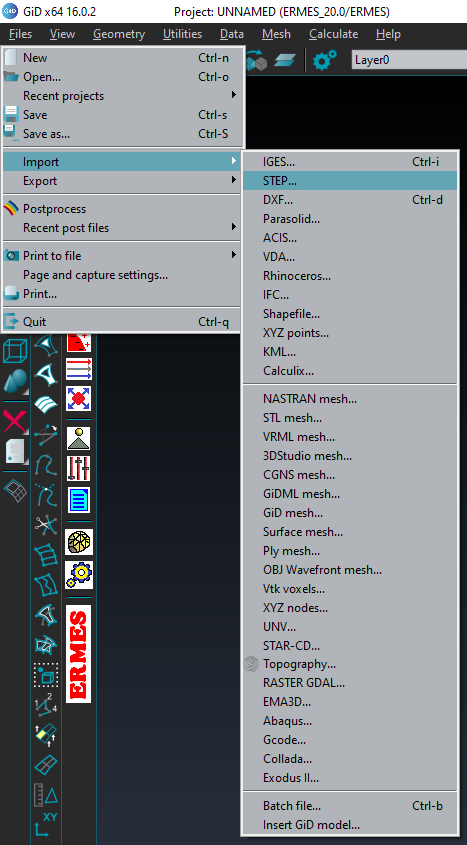
\includegraphics[width=0.72\textwidth]{Contents/Figures/GiD-ImportFormats.png}
		\caption{Supported CAD import formats in GiD.}\label{GiD-Formats}
	\end{center}
\end{figure}

\begin{figure}
	\begin{center}
		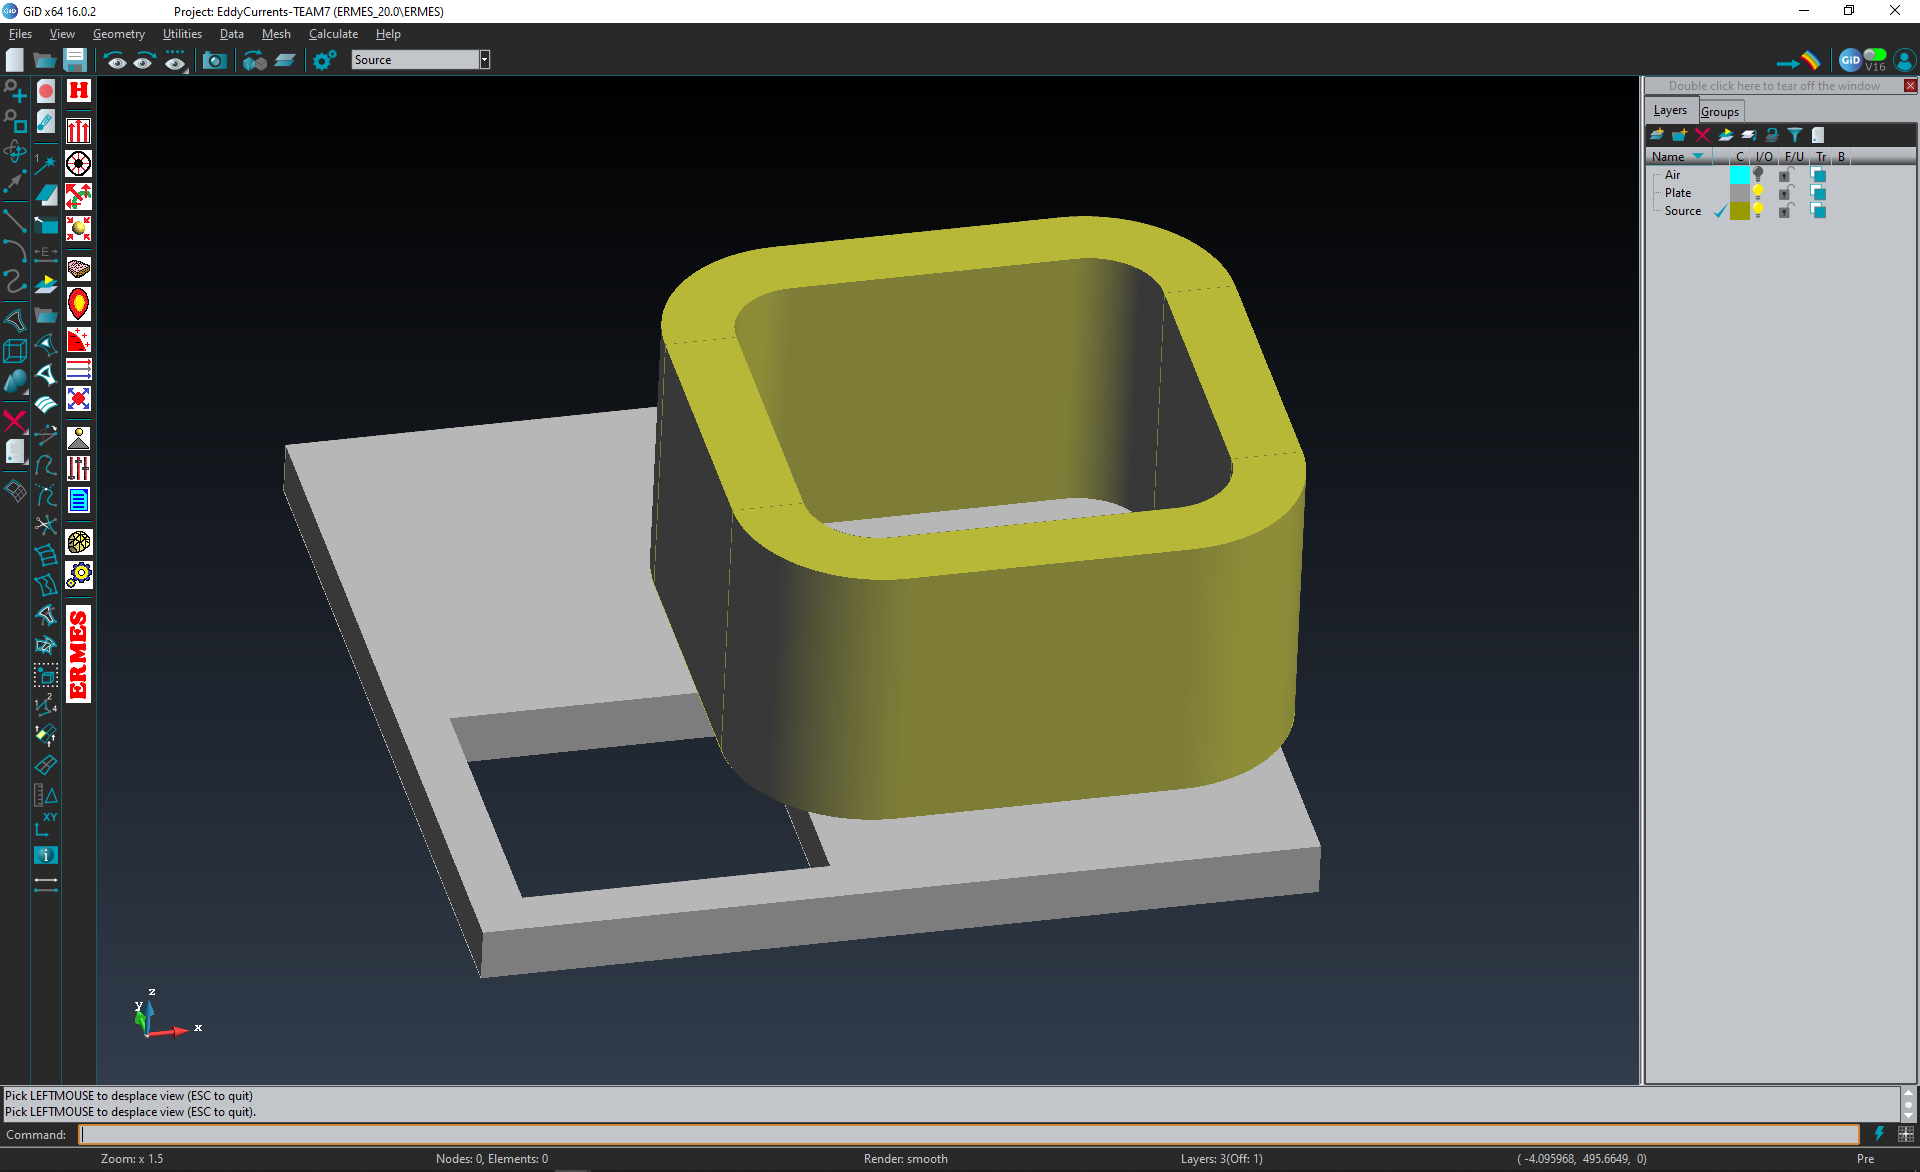
\includegraphics[width=0.87\textwidth]{Contents/Figures/GiD-GeoRender.png}
		\caption{CAD geometry of a coil and an asymmetrical conductive plate with a hole from the TEAM benchmark problem 7 (see description and results in \cite{TEAM7-Benchmark}). The geometry is shown using \textbf{Render} $\rightarrow$ \textbf{Flat mode} from the right mouse button contextual menu.}\label{GiD-GeoRender}
	\end{center}
\end{figure}

\begin{figure}
	\begin{center}
		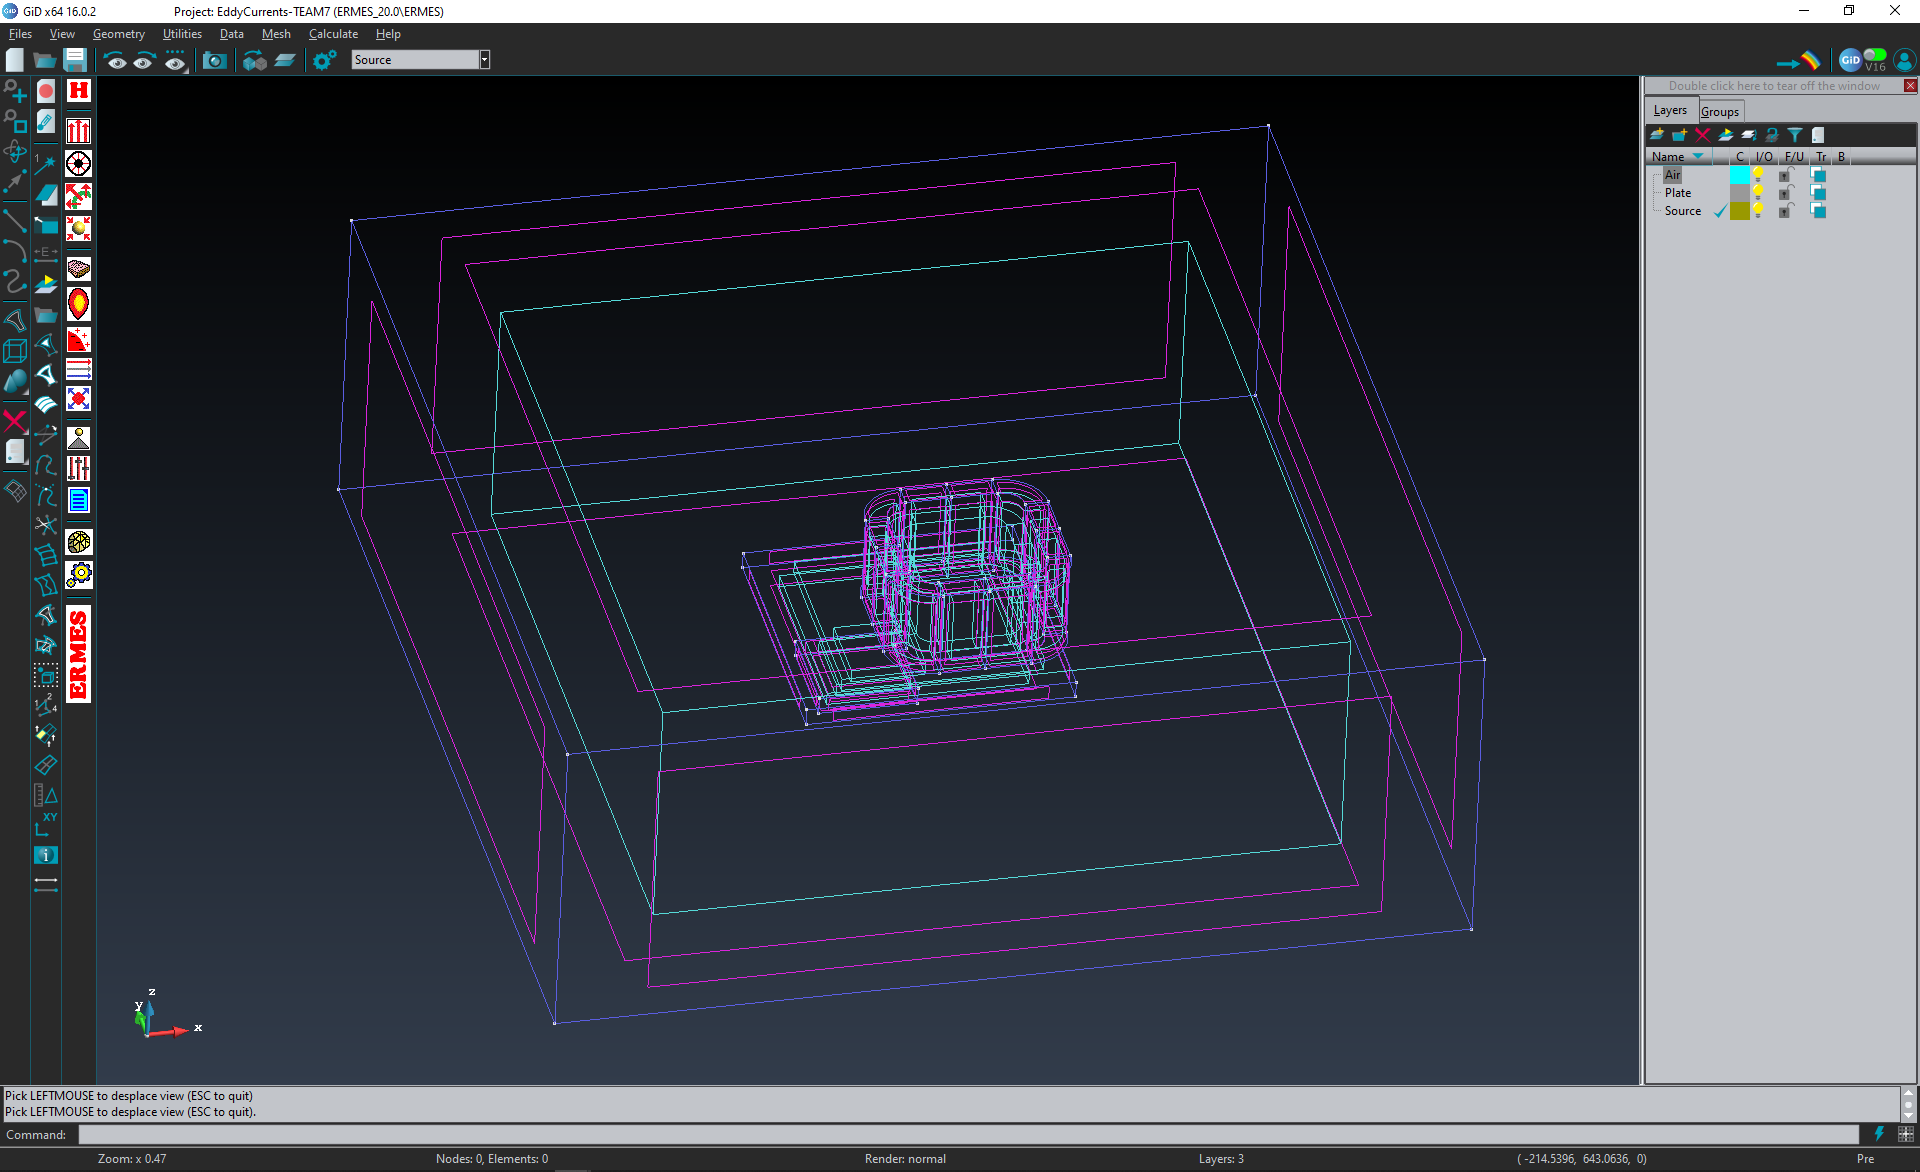
\includegraphics[width=0.87\textwidth]{Contents/Figures/GiD-GeoNoRender.png}
		\caption{Points (white), lines (blue), surfaces (purple) and, volumes (blue) of the geometry shown in Figure \ref{GiD-GeoRender} with an added volume of air surrounding the coil and plate. The geometry is shown using \textbf{Render} $\rightarrow$ \textbf{Normal mode} from the right mouse button contextual menu.}\label{GiD-GeoNoRender}
	\end{center}
\end{figure}

To create a CAD geometry inside GiD, it is advisable to follow first the tutorials provided in the GiD upper menu \textbf{\underline{H}elp} $\rightarrow$ \textbf{Tutorials...} or the tutorials and manuals available to download in \url{https://www.gidsimulation.com/gid-for-science/support/manuals/}. 

To import a geometry from a different CAD tool, go to the GiD upper menu and select \textbf{\underline{F}iles} $\rightarrow$ \textbf{Import}. Next, choose the appropriate format from the available options (see Figure \ref{GiD-Formats}).

After creating (or importing) the geometry, we must have a set of points, lines, surfaces, and volumes in where the materials, sources, and boundary conditions will be applied (see Figures \ref{GiD-GeoRender} and \ref{GiD-GeoNoRender}). The original geometry may need to be cleaned, repaired, or modified. For instance, we may need to add a volume to include the surrounding air, generate contact elements to allow nodal fields discontinuities (see Section \ref{Discontinuities}), or create separate contact volumes to define periodic boundary conditions. All these actions can be performed using GiD (check GiD tutorials and manuals for further information).

\section{ERMES menu bar}

All the input parameters required to run a simulation with ERMES 20.0 can be accessed from the menu bar shown in Figure \ref{ERMES-MenuBar}. It is advisable to go from top to bottom before starting a simulation, checking that all the necessary parameters have been defined and applied correctly. By clicking on the icons of Figure \ref{ERMES-MenuBar}, you will have access to the following:

\begin{figure}
	\begin{center}
		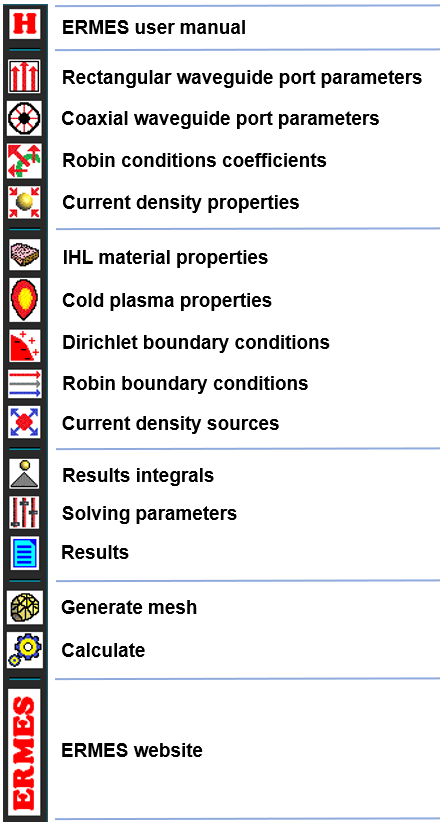
\includegraphics[width=0.69\textwidth]{Contents/Figures/ERMES-MenuBar-Ext.png}
		\caption{ERMES menu bar.}\label{ERMES-MenuBar}
	\end{center}
\end{figure}

\begin{enumerate}\itemsep0em 
	\item \textbf{ERMES user manual}: opens the user manual stored in \path{\Documents\Manual}. It may be necessary to set a PDF reader in your system to open it automatically.
	
	\item \textbf{Rectangular waveguide port parameters}: definition of the ports ID number, input power of the TE10 modes, location, and size of the rectangular waveguide ports. 
	
	\item \textbf{Coaxial waveguide port parameters}: definition of the ports ID number, input power of the TEM modes, location, and size of the coaxial waveguide ports. 

	\item \textbf{Robin conditions coefficients}: definition of the input parameters for plane waves and Gaussian beams, and  definition of the coefficients for generic quasi-static and electrostatic Robin boundary conditions. 

	\item \textbf{Current density properties}: definition of the module and phase of Cartesian, axisymmetric, helicoidal, and plasma current densities. 

	\item \textbf{IHL material properties}: definition of the complex electromagnetic properties of Isotropic Homogeneous Linear (IHL) materials (conductivity, permittivity, and permeability) and application to volumes. 

	\item \textbf{Cold plasma properties}: definition of cold plasma properties (i.e., geometry, paths to external files containing measured electron density and magnetic field, plasma composition, damping modes, and numerical tuning parameters) and application to volumes.

	\item \textbf{Dirichlet boundary conditions}: application to boundary surfaces, lines, or points of electric voltages, Perfect Electric Conductor (PEC) boundary conditions, Perfect Magnetic Conductor (PMC) boundary conditions, Periodic Boundary Conditions (PBC), Transversal Electric Conditions (TEC), and singularity layers.

	\item \textbf{Robin boundary conditions}: application to surfaces of far field boundary conditions, Robin boundary conditions, rectangular waveguide ports, and coaxial waveguide ports.

	\item \textbf{Current density sources}: application to volumes of electric current densities.

	\item \textbf{Results integrals}: selection of surfaces and volumes in where the result fields are going to be integrated to calculate average fields, total power, total current, and scattering parameters.

	\item \textbf{Solving parameters}: configuration of the global problem parameters (e.g., FEM formulation, stabilization mode, frequency, solver type, output file format).

	\item \textbf{Results}: selection of the results that are going to be stored in files and visualized in post-process.

	\item \textbf{Generate mesh}: generates a mesh of tetrahedral elements on the geometry.

	\item \textbf{Calculate}: writes the ERMES 20.0 input files and calls ERMES 20.0 to run the simulation.

	\item \textbf{ERMES website}: link to the last version of ERMES, manuals, documents, source code, executables, and simulation examples.
\end{enumerate}

\section{Materials}\label{Materials-Section}

In ERMES 20.0 there are implemented two types of materials:
\begin{enumerate}\itemsep0em 
	\item Isotropic Homogeneous Linear (IHL) materials,
	\item Cold plasma (inhomogeneous and gyrotropic).
\end{enumerate}
Material properties are defined in the windows \textit{IHL materials} and \textit{Plasma}, which can be open by clicking on the icons \textit{IHL material properties} and \textit{Cold plasma properties} of the menu bar shown in Figure \ref{ERMES-MenuBar}. Materials are assigned to volumes using the \textbf{\underline{A}ssign} button located in the same windows.

To assign a material, first click on \textbf{\underline{A}ssign} $\rightarrow$ \textbf{Volumes}. Then, select a volume as shown in Figure \ref{GiD-SelectVolume}. To confirm the application, click on the central mouse button, the keyboard key \textit{Escape}, or the \textit{Finish} button. To check if the material has been correctly assigned, click on \textbf{\underline{D}raw} $\rightarrow$ \textbf{All Materials} (located in the same material properties window). If properly assigned, the selected volume will appear in a solid colour as shown in Figure \ref{GiD-CheckMaterials}. 

\textbf{It is important to remember that all the volumes in the simulation domain must have a material assigned. If a volume does not have a material assigned, ERMES 20.0 will rise an error.}

To save the material data, create new materials, delete materials, rename, or get help, click on the buttons located at the upper part of the material property window. A short description of the button functionality will appear when hovering the mouse pointer above the button. Clicking on the help button and hovering above a material property will give a short description of that property.

\begin{figure}
	\begin{center}
		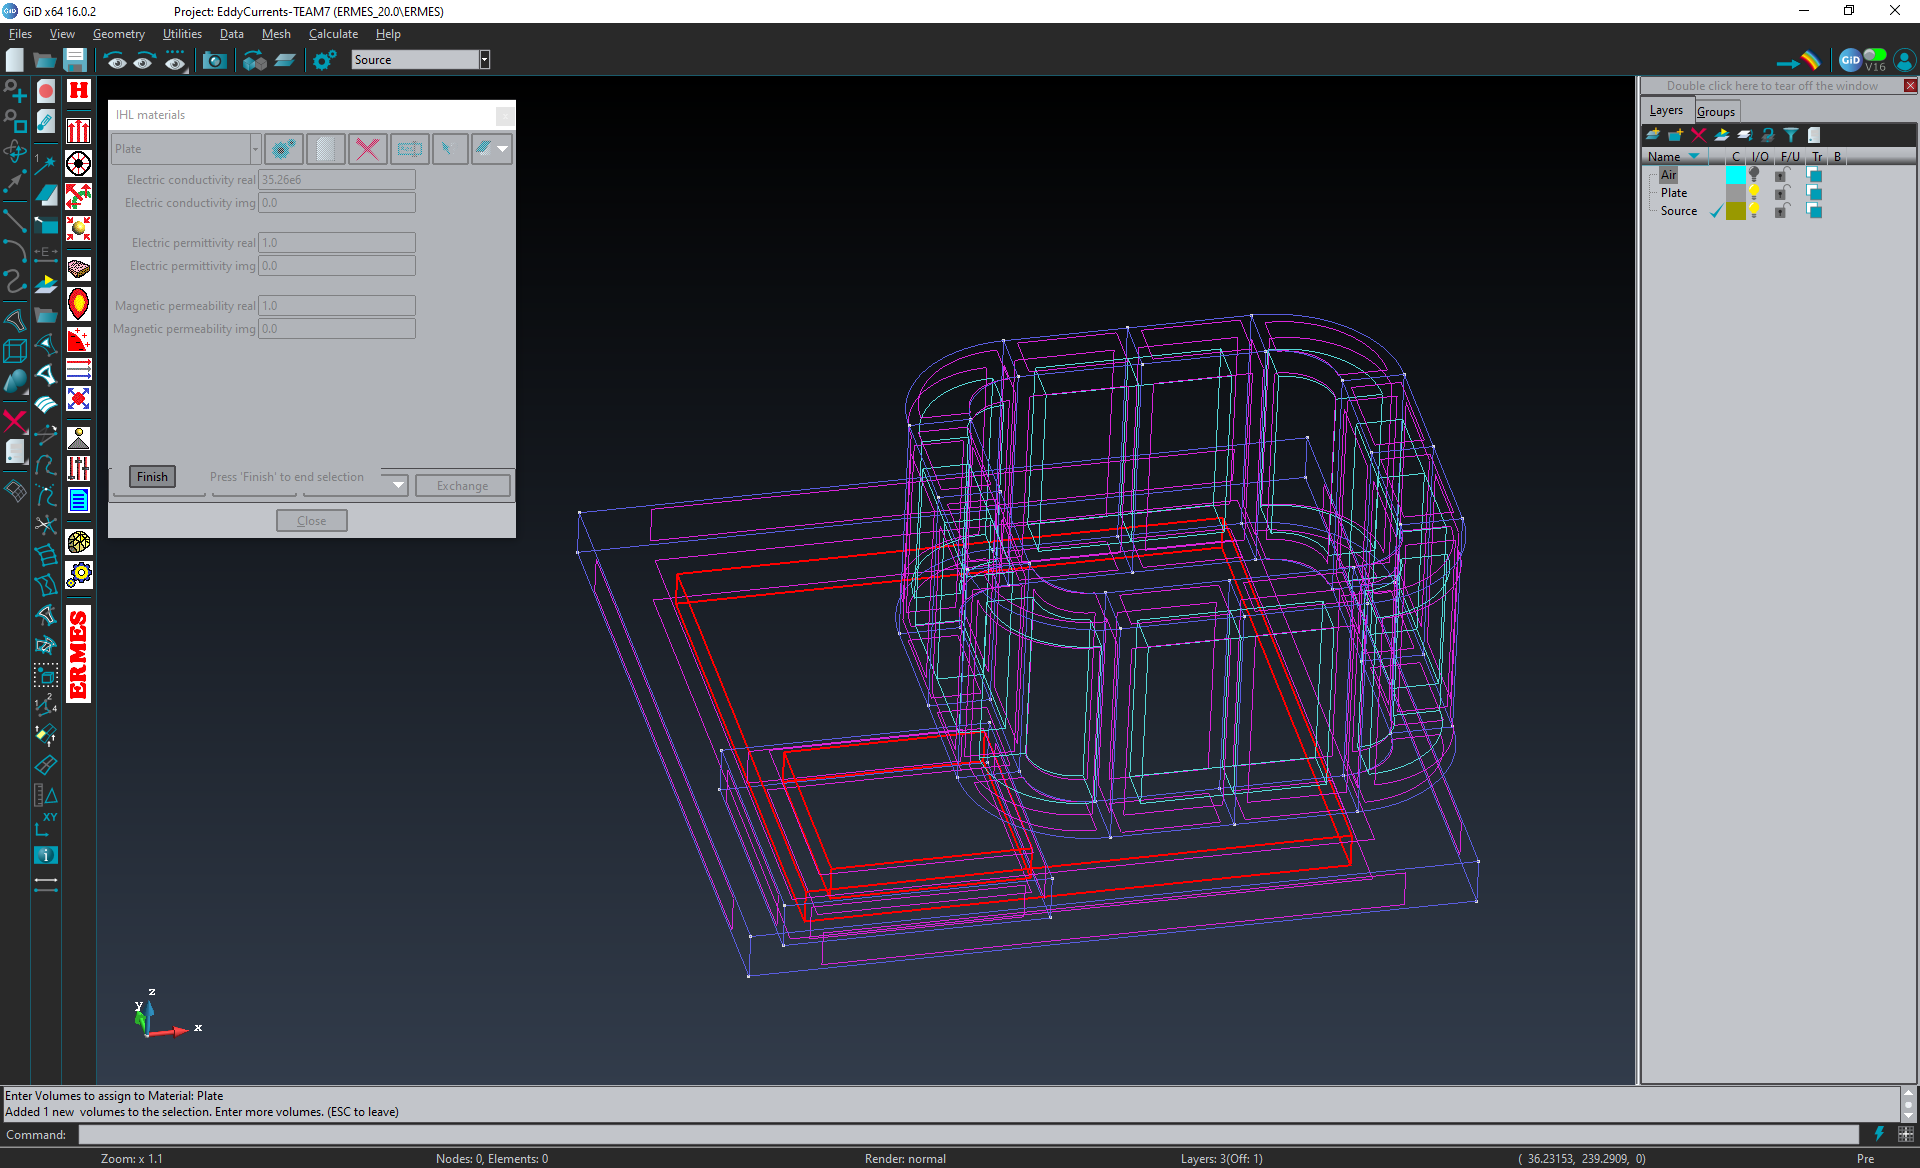
\includegraphics[width=0.89\textwidth]{Contents/Figures/GiD-SelectVolume.png}
		\caption{To assign a material, first click on \textbf{\underline{A}ssign} $\rightarrow$ \textbf{Volumes} (located in the same material properties window). Then, select a volume. The selected volume will appear in red. Then, click on the central mouse button, the keyboard key \textit{Escape}, or the \textit{Finish} button to confirm the application.}\label{GiD-SelectVolume}
	\end{center}
\end{figure}

\begin{figure}
	\begin{center}
		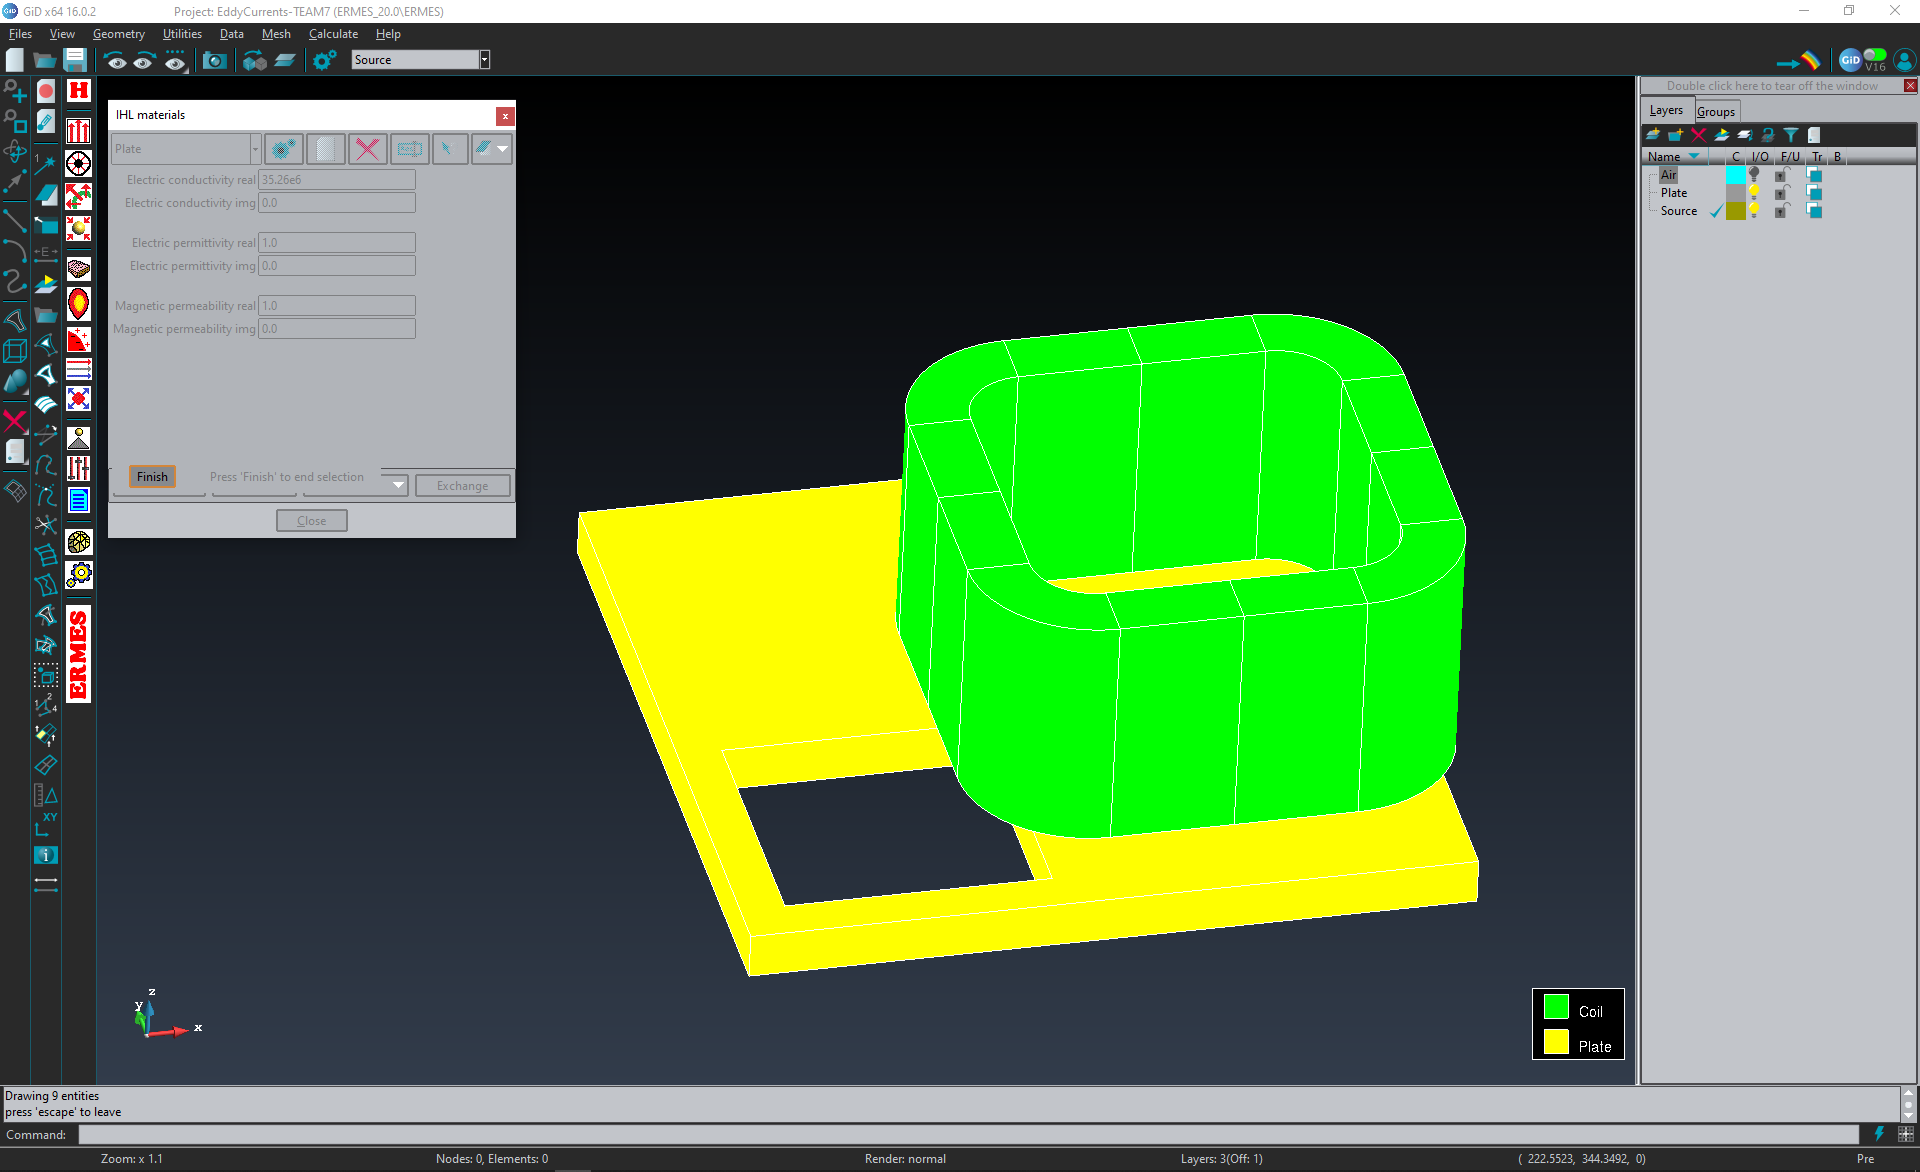
\includegraphics[width=0.89\textwidth]{Contents/Figures/GiD-CheckMaterials.png}
		\caption{To check if the materials has been correctly assigned, click on \textbf{\underline{D}raw} $\rightarrow$ \textbf{All Materials} (located in the same material window). The volumes will appear in solid colours if properly assigned.}\label{GiD-CheckMaterials}
	\end{center}
\end{figure}

\subsection{IHL materials}

Isotropic Homogeneous Linear (IHL) material properties are defined in the window \textit{IHL materials} shown in Figure \ref{Win-IHL-Materials}, which can be open from the icon \textit{IHL material properties} of the menu bar of Figure \ref{ERMES-MenuBar}. IHL materials are assigned to volumes using the \textbf{\underline{A}ssign} button located in the same \textit{IHL materials} window (see button on the lower left corner of Figure \ref{Win-IHL-Materials}). In ERMES 20.0, IHL materials are characterized by a complex permittivity $\varepsilon$ and a complex permeability $\mu$ \cite{Pozar, Jackson}:
\begin{equation}\label{ComplexPermittivityIHL}
    \varepsilon = \epsilon^{'} - \frac{\sigma^{''}}{\omega} + i\left(\epsilon^{''} + \frac{\sigma^{'}}{\omega}\right)
\end{equation}
\begin{equation}\label{ComplexPermeabiltyIHL}
    \mu = \mu^{'} + i \mu^{''}
\end{equation}
where:
\begin{itemize}\itemsep0em 
	\item $\sigma^{' }$: real part of the electric conductivity,
	\item $\sigma^{''}$: imaginary part of the electric conductivity,
    \\
	\item $\epsilon^{' }$: real part of the electric permittivity,
    \item $\epsilon^{''}$: imaginary part of the electric permittivity,
    \\
	\item $\mu^{' }$: real part of the magnetic permeability,
    \item $\mu^{''}$: imaginary part of the magnetic permeability.
\end{itemize}
These properties are related to the magnitudes in Figure \ref{Win-IHL-Materials} as follows:
\begin{itemize}\itemsep0em 
	\item \textbf{Electric conductivity real}: $\sigma^{' } \,\,\, \text{(S/m)}$,
	\item \textbf{Electric conductivity img }: $\sigma^{''} \,\,   \text{(S/m)}$,
    \\
	\item \textbf{Electric permittivity real}: $\epsilon_{r}^{' } \,\,\, (\epsilon^{' }\,/\epsilon_{0})$,
	\item \textbf{Electric permittivity img }: $\epsilon_{r}^{''} \,\,   (\epsilon^{''}/\epsilon_{0})$,
    \\
	\item \textbf{Magnetic permeability real}: $\mu_{r}^{' } \,\,\, (\mu^{' }\,/\mu_{0})$,
	\item \textbf{Magnetic permeability img }: $\mu_{r}^{''} \,\,   (\mu^{''}/\mu_{0})$.
\end{itemize}
where $\epsilon_{r}$ is the electric permittivity of the IHL material relative to the electric permittivity of vacuum $\epsilon_{0}$ and $\mu_{r}$ is the  magnetic permeability of the IHL material relative to magnetic permeability of vacuum $\mu_{0}$.

\subsection{Cold plasma}\label{ColdPlasmaMaterial}

Cold plasma properties are defined in the \textit{Plasma} window shown in Figures \ref{Win-ColdPlasma-1}, \ref{Win-ColdPlasma-2}, and \ref{Win-ColdPlasma-3}, which can be open by clicking on the icon \textit{Cold plasma properties} of the menu bar shown in Figure \ref{ERMES-MenuBar}. Cold plasma materials are assigned to volumes using the \textbf{\underline{A}ssign} button located in the same \textit{Plasma} window. Cold plasma materials will be only considered if the \textit{Cold plasma} problem mode is active (see Section \ref{ProblemSettings}), otherwise the volume will be considered the same as vacuum.

\textbf{Only one cold plasma material can be defined per simulation and almost one of the problem domain volumes must be assigned to this cold plasma material.} If a volume has an IHL material assigned with the same properties as vacuum then, that volume will be considered part of the cold plasma. On the other hand, if the IHL material assigned has different properties to vacuum (even tiny differences) then, that volume will be considered an IHL material and not part of the cold plasma. 

Applying different IHL materials to distinct volumes can be helpful to visualize the results in GiD post-process. Distinct volumes with different IHL materials assigned will be stored in separated layers by the GiD post-process. This separation happens even when the different materials have the same properties, or even when they have the same properties as vacuum and, therefore, are considered part of the cold plasma. The separation in layers makes easier the visualization of results because each layer can be displayed independently, which prevents one volume from blocking the view of another. 

The electron density distribution and the applied static \textbf{B} field are obtained from data files. The format of these data files will depend on the \textit{Geometry extrapolation} mode selected (see Figure \ref{Win-ColdPlasma-1} and its description in the next subsection). Examples of the different file formats can be found in the problemtype folder \path{\Documents\Plasma_Files} or in Section \ref{ColdPlasmaFiles}. 

For the 1D line file format, as a general rule, if the line starts with a number then, that line will be read and processed by ERMES. On the other hand, if a line starts with anything different from a number (e.g., a blank space, the symbol $\#$) then, that line will be considered a comment line and it will be ignored by ERMES. The numerical data columns must be separated by one or more blank spaces and the main precaution when writing the files is to avoid blank spaces at the beginning of a numerical data line (as mentioned before, a blank space at the beginning of a line will be interpreted as if the line is a comment).

For the 3D file format, the folder \path{\Documents\Plasma_Files} contains practical examples of Python scripts that can be used to transform \textit{eqdsk} equilibrium plasma files into the format required by ERMES 20.0.

The \textit{Plasma} window is divided in three tabs: \textit{Plasma geometry}, \textit{Species densities}, and \textit{Problem settings}. The \textit{Plasma geometry} tab is shown in Figure \ref{Win-ColdPlasma-1} and it used for specifying plasma extrapolation geometry types and the paths to files containing electron density distributions and the applied static \textbf{B} fields. The \textit{Species densities} tab is shown in Figure \ref{Win-ColdPlasma-2} and is where the plasma composition is defined. The \textit{Problem settings} tab is shown in Figure \ref{Win-ColdPlasma-3} and it is used for setting damping modes and tuning numerical parameters. The properties defined in each tab are described in the following subsections. Similar descriptions can be obtained inside GiD by hovering the mouse pointer over each data field after clicking on the help button located on the same \textit{Plasma} window.

\subsubsection{Plasma geometry - Figure \ref{Win-ColdPlasma-1}}\label{PlasmaGeometrySettings}

\begin{itemize}\itemsep0em 
	\item \textbf{Geometry extrapolation}: plasma geometry extrapolation type. It can be of three different types: 
	\begin{itemize}\itemsep1em 
	    \item \textbf{Flat 1D}: a 1D measurement line is read from the files specified in the \textit{ne file path} and \textit{Be file path} fields. The 1D line is extrapolated into the 3D geometry by extrusion in the toroidal direction, and applying a curvature in the poloidal direction defined by the \textit{Poloidal ne curvature} and \textit{Poloidal Be curvature} fields. The first point of the 1D measurement line will be placed at the coordinates specified in the \textit{L1 00 XYZ} fields. The values of \textit{ne} and \textit{Be} outside the defined line will correspond to those at the endpoints of the line.
	    \quad
	    \item \textbf{Curved}: a 1D measurement line is read from the files specified in the \textit{ne file path} and \textit{Be file path}. The 1D line is extrapolated into the 3D geometry by extrusion, applying a poloidal curvature defined by the \textit{Poloidal ne curvature} and \textit{Poloidal Be curvature} fields, and a toroidal curvature determined by the distance to the tokamak centre. The tokamak centre coordinates are specified in the \textit{TK 00 XYZ} fields. The first point of the 1D measurement line is placed at the coordinates defined in the \textit{L1 00 XYZ} fields. The values of \textit{ne} and \textit{Be} outside the defined line will correspond to those at the endpoints of the line.	    
	    \quad
	    \item \textbf{Full 3D}: pointwise nodal 3D distributions are read from the files specified in the \textit{ne file path} and \textit{Be file path} fields. The distributions are applied directly to the 3D geometry on a node-by-node basis.
	    \quad
	    \item \textbf{Tensor}: a permittivity tensor defined in the binary file \path{Tensor_K_CPGE.bin} is applied to the same mesh nodes used in the density and magnetic field 3D data files provided in the text boxes \textit{ne file path} and \textit{Be file path}. The tensor components must be relative to the vacuum permittivity and defined in the external \textbf{B} field coordinate system. The tensor file must be located in the problem folder. An example Python script demonstrating how to generate the required binary format can be found in the problem type directory \path{\Documents\Plasma_Files\Python_Scripts}.
    \end{itemize}
    \vspace{0.75em}
	\item \textbf{Poloidal ne curvature}: poloidal curvature applied to \textit{ne} density profile in the \textit{Flat 1D} and \textit{Curved} modes. The centre of curvature is located at a distance equal to the \textit{Poloidal ne curvature} from the first point of the 1D measurement line. The first point of the 1D measurement line is located at the coordinates specified in the \textit{L1 00 XYZ} fields.
	\vspace{1em}
	\item \textbf{Poloidal Be curvature}: poloidal curvature applied to the \textit{Be} field profile in the \textit{Flat 1D} and \textit{Curved} modes. The centre of curvature is located at a distance equal to the \textit{Poloidal Be curvature} from the first point of the 1D measurement line. The first point of the 1D measurement line is located at the coordinates specified in the \textit{L1 00 XYZ} fields.	
	\newpage
	\item \textbf{L1 00 X}: X coordinate of the first point of the 1D measurement line.
	\item \textbf{L1 00 Y}: Y coordinate of the first point of the 1D measurement line.
	\item \textbf{L1 00 Z}: Z coordinate of the first point of the 1D measurement line.
	\\
	\item \textbf{TK 00 X}: X coordinate of the centre of the tokamak.
	\item \textbf{TK 00 Y}: Y coordinate of the centre of the tokamak.
	\item \textbf{TK 00 Z}: Z coordinate of the centre of the tokamak.
	\\
	\item \textbf{TK axis X}: X component of the main axis of the tokamak.
    \item \textbf{TK axis Y}: Y component of the main axis of the tokamak.
    \item \textbf{TK axis Z}: Z component of the main axis of the tokamak.
    \\
    \item \textbf{ne file path}: electron density data file path.
    \item \textbf{Be file path}: applied external static \textbf{B} field data file path.
\end{itemize}

\subsubsection{Plasma composition - Figure \ref{Win-ColdPlasma-2}}

\begin{itemize}\itemsep0em 
	\item \textbf{H1 1+ / ne}: Hydrogen 1 (protium) ion q=+1e density relative to electron density (ne).
	\item \textbf{H2 1+ / ne}: Hydrogen 2 (deuterium) ion q=+1e density relative to electron density (ne).
	\item \textbf{H3 1+ / ne}: Hydrogen 3 (tritium) ion q=+1e density relative to electron density (ne).
	\\
	\item \textbf{He3 1+ / ne}: Helium 3 ion q=+1e density relative to electron density (ne).
    \item \textbf{He3 2+ / ne}: Helium 3 ion q=+2e density relative to electron density (ne).
    \\
    \item \textbf{He4 1+ / ne}: Helium 4 ion q=+1e density relative to electron density (ne).
    \item \textbf{He4 2+ / ne}: Helium 4 ion q=+2e density relative to electron density (ne).
    \\
	\item \textbf{Be9 1+ / ne}: Beryllium 9 ion q=+1e density relative to electron density (ne).
    \item \textbf{Be9 2+ / ne}: Beryllium 9 ion q=+2e density relative to electron density (ne).
    \item \textbf{Be9 3+ / ne}: Beryllium 9 ion q=+3e density relative to electron density (ne).
    \item \textbf{Be9 4+ / ne}: Beryllium 9 ion q=+4e density relative to electron density (ne).
    \\
	\item \textbf{Ne20 \,10+ \,/ ne}: Neon 20 ion q=+10e density relative to electron density (ne).
    \item \textbf{Ni60 \, 20+ \,/ ne}: Nickel 60 ion q=+20e density relative to electron density (ne).
    \item \textbf{W184 25+ / ne}: Tungsten 184 ion q=+25e density relative to electron density (ne).
\end{itemize}

\subsubsection{Plasma problem settings - Figure \ref{Win-ColdPlasma-3}}\label{ColdPlasmaSettings}

\begin{itemize}\itemsep1em 
	\item \textbf{Matrix format}: available storage formats for the cold plasma system matrix:
	\begin{itemize}\itemsep0.75em 
		\item \textbf{Full matrix}: stores a non-symmetric matrix containing the contribution of the volumetric and the Robin boundary condition elements altogether.
		\quad
		\item \textbf{Herm-Full}: stores two separate matrices containing the diagonal and the upper diagonal of the volumetric elements contribution and, a non-symmetric matrix with the contribution of the Robin boundary condition elements.
		\quad
		\item \textbf{Herm-Symm}: stores two separate matrices containing the diagonal and the upper diagonal of the volumetric elements contribution and, the diagonal and the upper diagonal of the Robin boundary condition elements contribution.
	\end{itemize}
	\item \textbf{Kij tolerance}: minimum value of the elements of the matrix. If $\mid K_{ij} \mid\, <= Tol$ then, $K_{ij}$ will not be added to the global system matrix.
	\item \textbf{E par tolerance}: tolerance applied to the electric field parallel to the magnetic flux density: $\textbf{E}_{\parallel} = 0$ when $P < 0$ and $\mid P \mid\, > Tol$. This condition will be ignored in the edge element formulations. 
	\item \textbf{Damping mode}: available damping modes:
	\begin{itemize}\itemsep0.75em 
	    \item \textbf{No damping}: no damping is applied to the cold plasma tensor.
	    \quad
	    \item \textbf{Background ctc}: a constant damping value $\nu$ is added to the diagonal terms of the cold plasma tensor ($R + i\nu$, $L + i\nu$, $P + i\nu$, $S + i\nu$) everywhere the cold plasma is defined.
	    \quad
	    \item \textbf{Background den}: as in the \emph{Background ctc} mode, a constant damping value $\nu$ is added to the diagonal terms of the cold plasma tensor ($R + i\nu$, $L + i\nu$, $P + i\nu$, $S + i\nu$) but, in this case, the damping value $\nu$ is made zero when the electron density is zero.
	    \quad
	    \item \textbf{ComplexFreq all}: a collision frequency $\nu$ is added to the frequency terms of all the species ($\omega + i\nu$), as shown in \cite{Swanson}
	    \quad
	    \item \textbf{ComplexFreq ele}: as in the \emph{ComplexFreq all} mode, a collision frequency $\nu$ is added to the frequency terms ($\omega + i\nu$) but, in this case, only in the electrons contribution to the cold plasma tensor.
    \end{itemize}	
	\item \textbf{Damping value}: damping value $\nu$. It has a different meaning depending on the damping mode selected.
\end{itemize}

\newpage

\begin{figure}[H]
	\begin{center}
		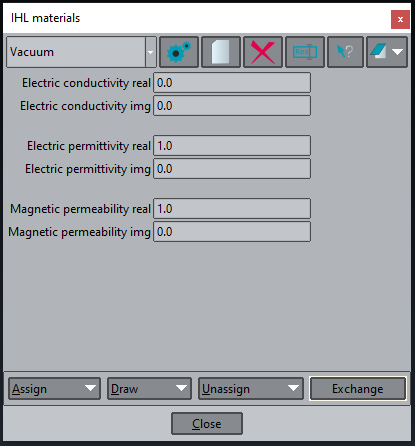
\includegraphics[width=0.40\textwidth]{Contents/Figures/Win-IHL-Materials.png}
		\caption{Isotropic Homogeneous Linear (IHL) material properties window.}\label{Win-IHL-Materials}
	\end{center}
\end{figure}

\begin{figure}[H]
	\begin{center}
		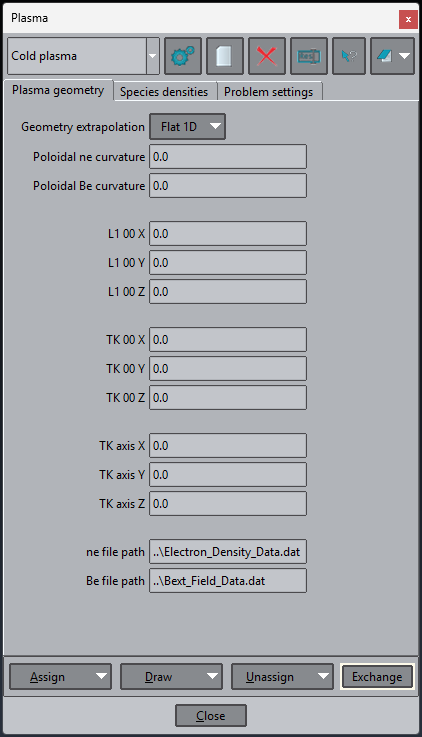
\includegraphics[width=0.40\textwidth]{Contents/Figures/Win-ColdPlasma-1.png}
		\caption{Cold plasma properties window - Tab: Plasma geometry.}\label{Win-ColdPlasma-1}
	\end{center}
\end{figure}

\begin{figure}[H]
	\begin{center}
		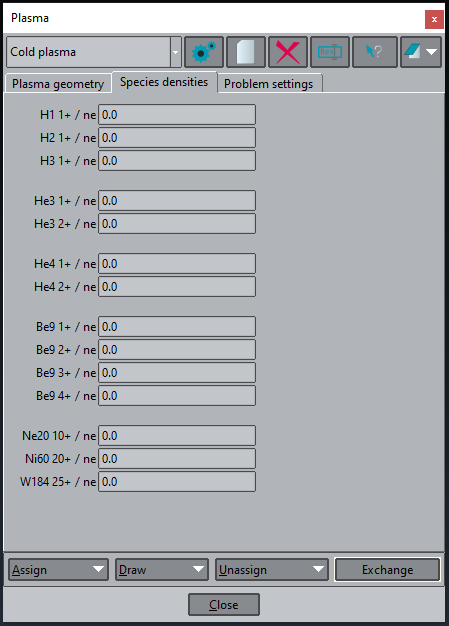
\includegraphics[width=0.40\textwidth]{Contents/Figures/Win-ColdPlasma-2.png}
		\caption{Cold plasma properties window - Tab: Species densities.}\label{Win-ColdPlasma-2}
	\end{center}
\end{figure}

\begin{figure}[H]
	\begin{center}
		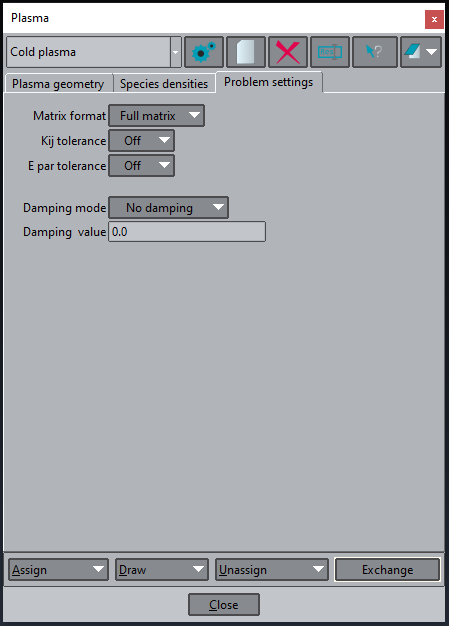
\includegraphics[width=0.40\textwidth]{Contents/Figures/Win-ColdPlasma-3.png}
		\caption{Cold plasma properties window - Tab: Problem settings.}\label{Win-ColdPlasma-3}
	\end{center}
\end{figure}

\section{Sources}

In ERMES 20.0 there are implemented two types of electromagnetic field sources: 
\begin{enumerate}\itemsep0em 
	\item Volumetric sources (electric current density vectors \textbf{J}).
	\item Boundary sources (plane waves, Gaussian beams, waveguide modes, current flux).
\end{enumerate}
Volumetric sources are electric current densities \textbf{J} applied to volumes inside the problem domain. Boundary sources are electromagnetic fields applied as Robin conditions to the boundary surfaces of the problem domain (e.g., plane waves, Gaussian beams, waveguide modes, current flux). 

\textbf{All the sources must be first defined on its corresponding properties window and then applied to volumes (or surfaces) using its associated conditions window. The sources assignment process is different from the materials assignment process explained in Section \ref{Materials-Section}. Materials are defined and assigned from the same window. On the other hand, sources are defined in a properties definition window and assigned from a conditions window.} Further details will be given in the following sections.

\subsection{Volumetric sources J}

Current density \textbf{J} sources properties are defined in the window \textit{Current sources properties} shown in Figures \ref{Win-J-Cartesian}, \ref{Win-J-Axisymm}, \ref{Win-J-Combine}, \ref{Win-J-Helicoidal}, and \ref{Win-J-PlasmaM}, which can be opened from the menu bar of Figure \ref{ERMES-MenuBar} by clicking on the icon \textit{Current density properties} \ref{Source-Properties-Icon}. To create a new \textbf{J}, click on the white paper sheet icon button at the upper part of the \textit{Current sources properties} window.

Once the properties of \textbf{J} have been defined in the \textit{Current sources properties} window, the \textbf{J} source must be assigned to a volume from the \textit{Current sources} window of Figure \ref{Win-J-ApplySource}, which can be opened from the ERMES menu bar by clicking on the \textit{Current density sources} icon \ref{Apply-Sources-Icon}. 

Current density \textbf{J} sources are applied to volumes following a procedure similar to the one explained in Section \ref{Materials-Section} and shown in Figure \ref{GiD-SelectVolume}, but using the window \textit{Current sources} of Figure \ref{Win-J-ApplySource} instead. The \textbf{J} source assigned to the volume will be the one selected in the drop-down menu of Figure \ref{Win-J-ApplySource}.

For checking the correct application of \textbf{J} sources, click on the  \textbf{\underline{D}raw} $\rightarrow$ \textbf{Colors} menu located at the bottom of the \textit{Current sources} window of Figure \ref{Win-J-ApplySource}. If properly assigned, the selected volume will appear in a solid colour along with the other \textbf{J} sources assigned, as shown in Figure \ref{GiD-SourceChecking}. 

\textbf{It is important to remember that the current sources properties window must only be used to define the \textbf{J} source properties, not to assign the \textbf{J} source to a volume. Assigning a current density to a volume from the \textit{Current sources properties} window will raise an error in ERMES 20.0.} In the following subsections will be described the parameters required to define the complex electric current density vector \textbf{J} on different coordinate systems from the window \textit{Current sources properties}.

\begin{figure}[H]
	\begin{center}
		
\includegraphics[width=0.05\textwidth]{Contents/Figures/Source-Properties-Icon.png}
		\caption{ERMES menu bar icon to access the \textit{Current sources properties} windows shown in \ref{Win-J-Cartesian}, \ref{Win-J-Axisymm}, \ref{Win-J-Combine}, \ref{Win-J-Helicoidal}, and \ref{Win-J-PlasmaM}.}\label{Source-Properties-Icon}
	\end{center}
\end{figure}

\vspace{-1.15cm}

\begin{figure}[H]
	\begin{center}
		
\includegraphics[width=0.05\textwidth]{Contents/Figures/Apply-Sources-Icon.png}
		\caption{ERMES menu bar icon to access the \textit{Current sources} assignment window \ref{Win-J-ApplySource}.}\label{Apply-Sources-Icon}
	\end{center}
\end{figure}

\vspace{-0.55cm}

\begin{figure}[H]
	\begin{center}
		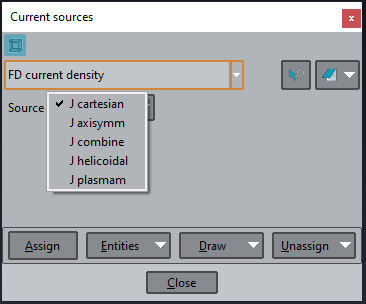
\includegraphics[width=0.5\textwidth]{Contents/Figures/Win-J-Assign.png}
		\caption{Electric current density \textbf{J} assignment window. \textbf{J} sources must be assigned to volumes using the \textbf{\underline{A}ssign} button located on the lower left corner of the \textit{Current sources} window.}\label{Win-J-ApplySource}
	\end{center}
\end{figure}

\vspace{-0.55cm}

\begin{figure}[H]
	\begin{center}
		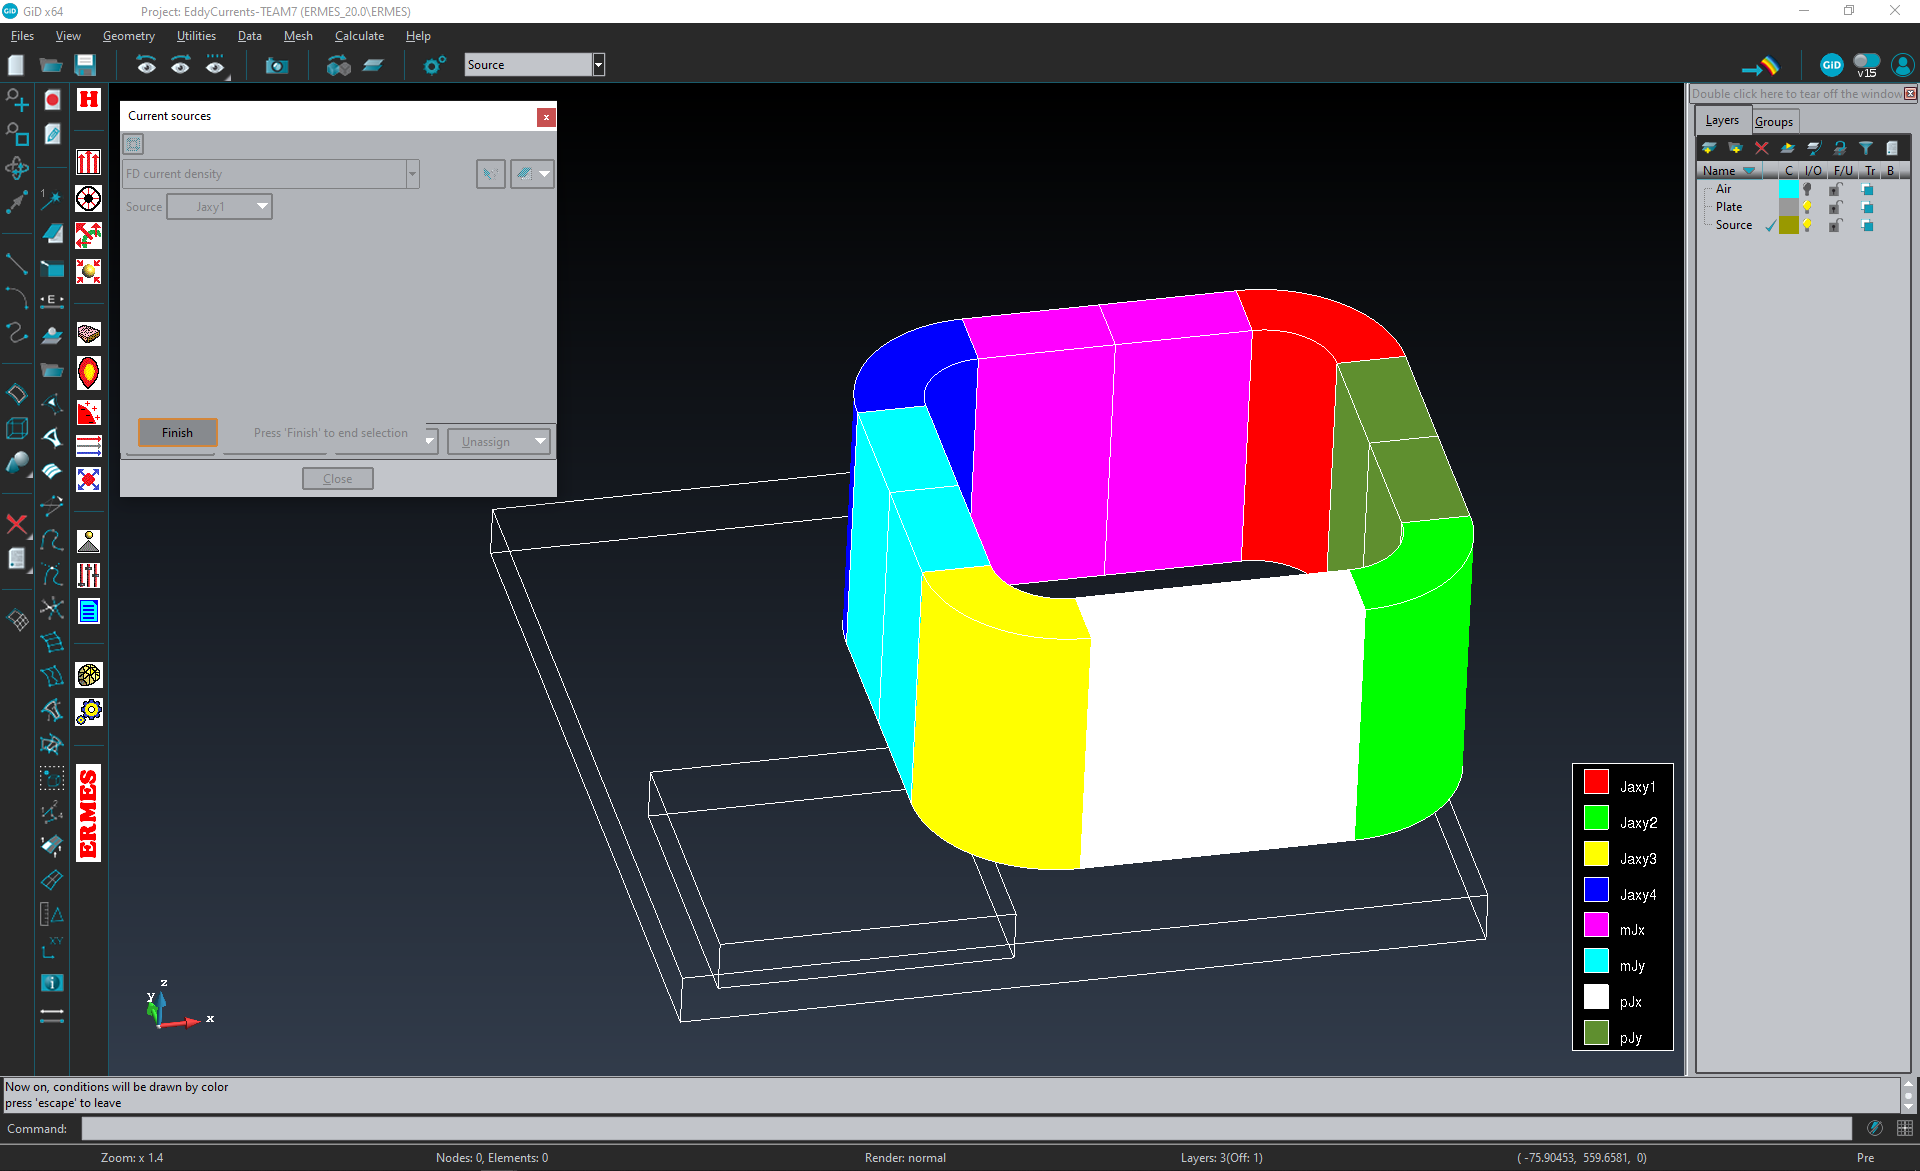
\includegraphics[width=0.7\textwidth]{Contents/Figures/GiD-SourceChecking.png}
		\caption{Assigned electric current densities \textbf{J}. To check the correct assignment of \textbf{J} sources, click on the \textbf{\underline{D}raw} $\rightarrow$ \textbf{Colors} menu located at the bottom of the \textit{Current sources} window of Figure \ref{Win-J-ApplySource}.}\label{GiD-SourceChecking}
	\end{center}
\end{figure}

\subsubsection{J Cartesian - Figure \ref{Win-J-Cartesian}}

Complex electric current density vector $\textbf{J}_{xyz}$ in Cartesian coordinates:
\begin{itemize}\itemsep0em 
	\item \textbf{Jx }: modulus of the X component of the electric current density vector (A/m$^{2}$).
	\item \textbf{Phx}: phase of the X component of the electric current density (rad).
	\\
	\item \textbf{Jy }: modulus of the Y component of the electric current density vector (A/m$^{2}$).
	\item \textbf{Phy}: phase of the Y component of the electric current density (rad).
	\\
	\item \textbf{Jz }: modulus of the Z component of the electric current density vector (A/m$^{2}$).
	\item \textbf{Phz}: phase of the Z component of the electric current density (rad).
\end{itemize}

\subsubsection{J axisymmetric - Figure \ref{Win-J-Axisymm}}

Complex electric current density vector $\textbf{J}_{a}$ in axisymmetric coordinates. $\textbf{J}_{a}$ is axisymmetric with respect to the axis defined in \emph{AX axis XYZ} with centre of curvature on \emph{AX 00 XYZ}:
\begin{itemize}\itemsep0em 
	\item \textbf{Ja }: modulus of the angular component of the axisymmetric current density vector (A/m$^{2}$). 
	\item \textbf{Pha}: phase of the angular component of the axisymmetric current density vector (rad).
	\\
	\item \textbf{AX 00 X}: X coordinate of the centre of curvature.
	\item \textbf{AX 00 Y}: Y coordinate of the centre of curvature.
	\item \textbf{AX 00 Z}: Z coordinate of the centre of curvature.
	\\
	\item \textbf{AX axis X}: X component of the axisymmetric axis.
	\item \textbf{AX axis Y}: Y component of the axisymmetric axis.
	\item \textbf{AX axis Z}: Z component of the axisymmetric axis.
\end{itemize}

\subsubsection{J Cartesian and axisymmetric - Figure \ref{Win-J-Combine}}

Combination of a complex electric current density vector $\textbf{J}_{xyz}$ in Cartesian coordinates plus a complex electric current density vector $\textbf{J}_{a}$ in axisymmetric coordinates. Both current densities will be assigned to the same volume and added to create a total current equal to the combination of the two: $\textbf{J}_{combine} = \textbf{J}_{xyz} + \textbf{J}_{a}$. The definitions of properties for $\textbf{J}_{combine}$ in Figure \ref{Win-J-Combine} are the same as the ones shown in Figures \ref{Win-J-Cartesian} and \ref{Win-J-Axisymm}. To access to the properties of $\textbf{J}_{a}$ click on the \textit{Axisymmetric} tab of Figure \ref{Win-J-Combine}.

\subsubsection{J helicoidal - Figure \ref{Win-J-Helicoidal}}

This input window allows to set a volumetric current density in both poloidal and toroidal directions $\textbf{J}_{heli} = \textbf{J}_{pol} + \textbf{J}_{tor}$. The current density $\textbf{J}_{heli}$ will be applied to a torus volume with a major radius \emph{HL R}, centered at \emph{HL 00 XYZ}, around the axis \emph{HL axis XYZ}:
\begin{itemize}\itemsep0em 
	\item \textbf{Jpol}: module of the poloidal component of the helicoidal current density (A/m$^{2}$). 
	\item \textbf{Php }: phase of the poloidal component of the helicoidal current density (rad).
	\\
	\item \textbf{Jtor}: module of the toroidal component of the helicoidal current density (A/m$^{2}$). 
    \item \textbf{Pht }: phase of the toroidal component of the helicoidal current density (rad).
    \\
    \item \textbf{HL R}: major radius of the torus in where the helicoidal current is applied.
    \\
	\item \textbf{HL 00 X}: X coordinate of the torus centre.
	\item \textbf{HL 00 Y}: Y coordinate of the torus centre.
	\item \textbf{HL 00 Z}: Z coordinate of the torus centre.
	\\
	\item \textbf{HL axis X}: X component of the torus axis.
	\item \textbf{HL axis Y}: Y component of the torus axis.
	\item \textbf{HL axis Z}: Z component of the torus axis.
\end{itemize}

\subsubsection{J plasma modes - Figure \ref{Win-J-PlasmaM}}

This input window sets a volumetric current density $\textbf{J}_{plasm} = \textbf{J}_{pol} + \textbf{J}_{tor}$ defined in a torus volume with a major radius \emph{PM R}, centered at \emph{PM 00 XYZ}, around the axis \emph{PM axis XYZ}. The current densities $\textbf{J}_{pol}$ and $\textbf{J}_{tor}$ satisfy the following equations:
\begin{equation}\label{PlasmaModeJ}
	\begin{aligned}
		\mathbf{J_{pol}} &= \left|\mathbf{A}_{0}\right|e^{i\varphi_{0}}\sin\left(M\theta+\phi\right)
		\\
		\mathbf{J_{tor}} &= \left|\mathbf{B}_{0}\right|e^{i\psi_{0}}\left\lbrace-M\left[\left(R/r\right) + \cos\left(\theta\right)\right]\sin\left(M\theta+\phi\right) - \sin(\theta)\cos\left( M\theta+\phi\right)\right\rbrace 
	\end{aligned}
\end{equation}
where $\mathbf{A}_{0} = \left|\mathbf{A}_{0}\right|e^{i\varphi_{0}}$ and $\mathbf{B}_{0} = \left|\mathbf{B}_{0}\right|e^{i\psi_{0}}$ are complex constants scaling $\mathbf{J_{pol}}$ and $\mathbf{J_{tor}}$, respectively, $M$ is an integer number representing the current density mode, $\theta$ is the poloidal angle, $\phi$ is the toroidal angle, $R$ is the major radius of the torus and, $r$ is its minor radius. Figures \ref{PlasmaModesExamples-1} and \ref{PlasmaModesExamples-2} present examples of $\textbf{J}_{plasm}$ for various mode numbers. The parameters required to configure $\textbf{J}_{plasm}$ using the interface shown in Figure \ref{Win-J-PlasmaM} are described below:
\quad\\
\begin{itemize}\itemsep0em 
	\item \textbf{Jpol}: module of the constant complex number $\mathbf{A}_{0}$ (A/m$^{2}$). 
	\item \textbf{Php }: phase $\varphi_{0}$ (rad) of the constant complex number $\mathbf{A}_{0}$.
	\\
	\item \textbf{Jtor}: module of the constant complex number $\mathbf{B}_{0}$ (A/m$^{2}$). 
	\item \textbf{Pht }: phase $\psi_{0}$ (rad) of the constant complex number $\mathbf{B}_{0}$.
	\\
	\item \textbf{PM M}: plasma mode index.
	\item \textbf{PM R}: major radius of the torus in where the plasma mode is applied.
	\\
	\item \textbf{PM 00 X}: X coordinate of the torus centre.
	\item \textbf{PM 00 Y}: Y coordinate of the torus centre.
	\item \textbf{PM 00 Z}: Z coordinate of the torus centre.
	\\
	\item \textbf{PM axis X}: X component of the torus axis.
	\item \textbf{PM axis Y}: Y component of the torus axis.
	\item \textbf{PM axis Z}: Z component of the torus axis.
\end{itemize}
\quad\\

\begin{figure}[H]
	\begin{center}
		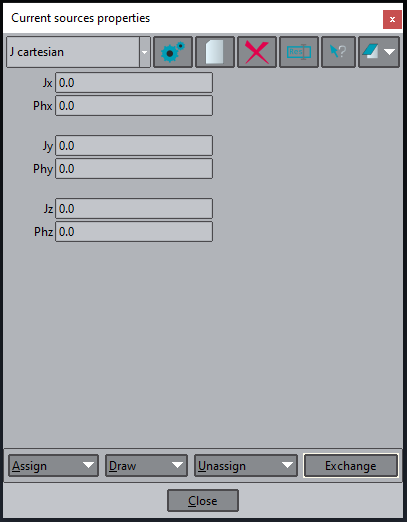
\includegraphics[width=0.45\textwidth]{Contents/Figures/Win-J-Cartesian.png}
		\caption{Current sources properties window - \textbf{J} Cartesian.}\label{Win-J-Cartesian}
	\end{center}
\end{figure}

\begin{figure}[H]
	\begin{center}
		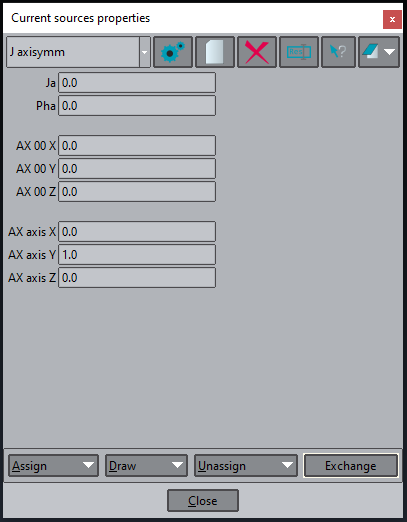
\includegraphics[width=0.43\textwidth]{Contents/Figures/Win-J-Axisymm.png}
		\caption{Current sources properties window - \textbf{J} axisymm.}\label{Win-J-Axisymm}
	\end{center}
\end{figure}

\begin{figure}[H]
	\begin{center}
		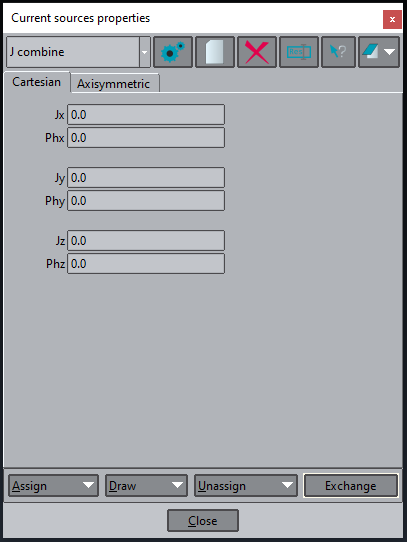
\includegraphics[width=0.43\textwidth]{Contents/Figures/Win-J-Combine.png}
		\caption{Current sources properties window - \textbf{J} combine.}\label{Win-J-Combine}
	\end{center}
\end{figure}

\begin{figure}[H]
	\begin{center}
		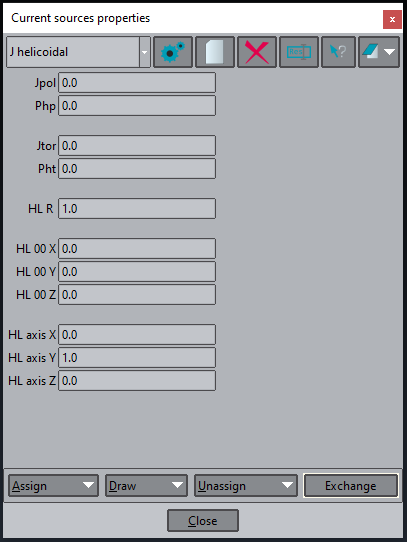
\includegraphics[width=0.42\textwidth]{Contents/Figures/Win-J-Helicoidal.png}
		\caption{Current sources properties window - \textbf{J} helicoidal.}\label{Win-J-Helicoidal}
	\end{center}
\end{figure}

\begin{figure}[H]
	\begin{center}
		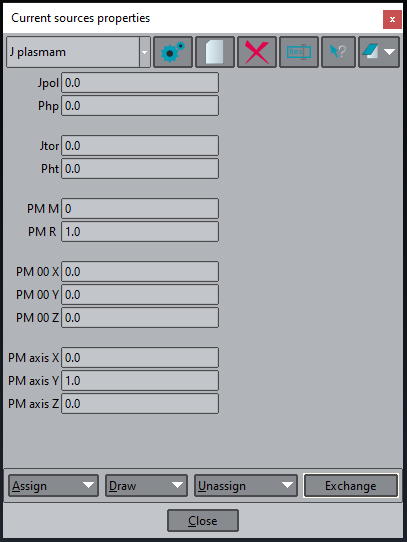
\includegraphics[width=0.42\textwidth]{Contents/Figures/Win-J-PlasmaM.png}
		\caption{Current sources properties window - \textbf{J} plasmam.}\label{Win-J-PlasmaM}
	\end{center}
\end{figure}

\begin{figure}[H]
	\begin{center}
		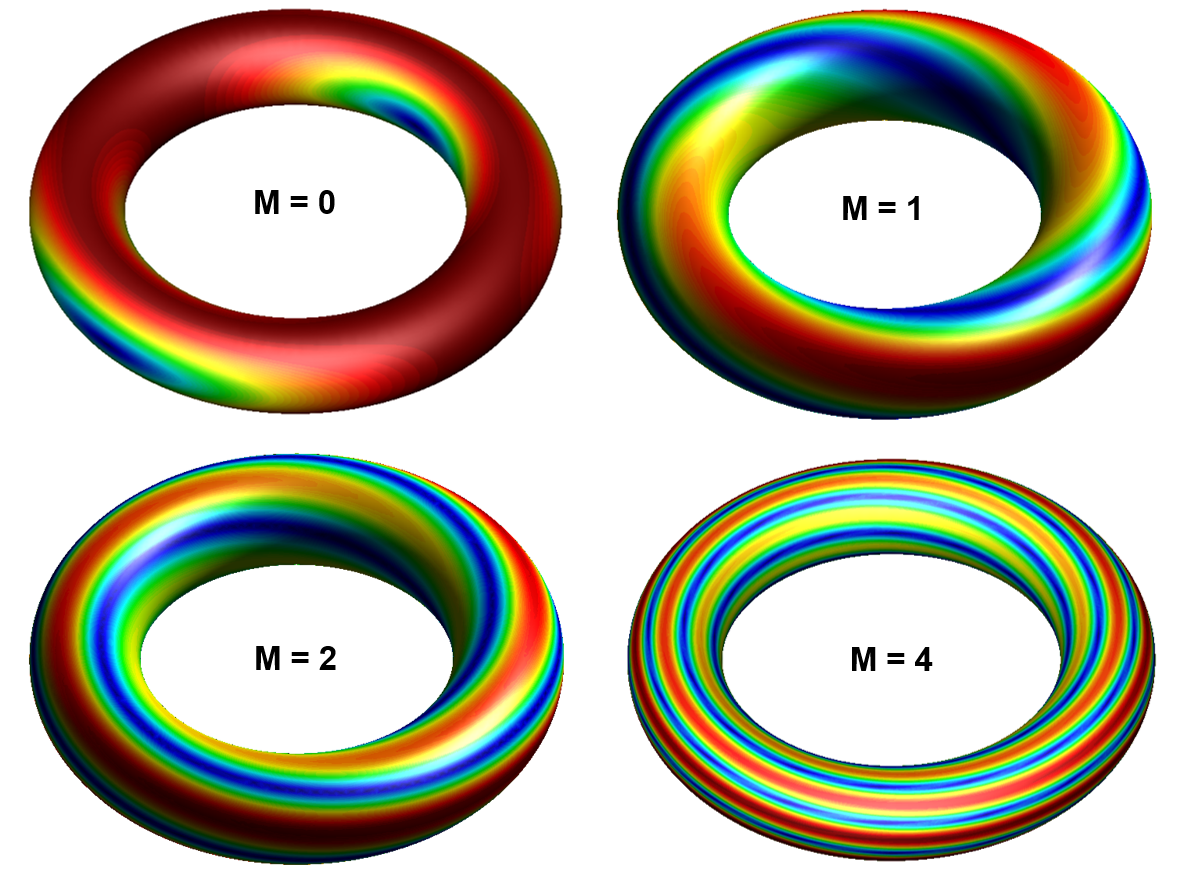
\includegraphics[width=\textwidth]{Contents/Figures/PlasmaJModes.png}
		\caption{Module of $\textbf{J}_{plasm}$ for M = 0, 1, 2 and, 4.}\label{PlasmaModesExamples-1}
	\end{center}
\end{figure}

\begin{figure}[H]
	\begin{center}
		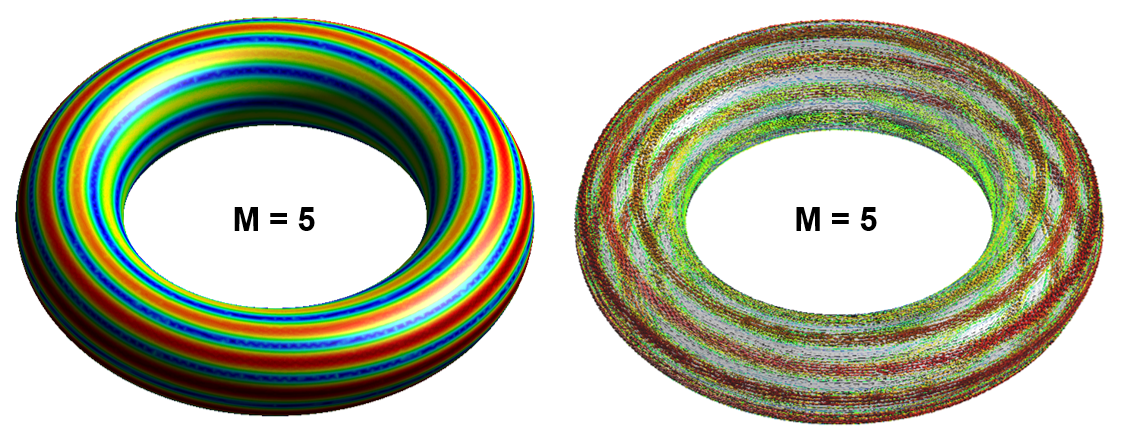
\includegraphics[width=\textwidth]{Contents/Figures/PlasmaJModes-M5.png}
		\caption{Module and vectors of $\textbf{J}_{plasm}$ for M = 5.}\label{PlasmaModesExamples-2}
	\end{center}
\end{figure}

\subsection{Boundary sources}\label{ssBoundarySources}

Boundary sources are fields applied at the boundaries of the problem domain using Robin boundary conditions. This section outlines the properties required by ERMES 20.0 to define these sources. Appendix \ref{chEMTheory} provides theoretical background on these conditions in the context of electromagnetics. Appendix \ref{chFEMForms} describes their adaptation to the various FEM formulations implemented in ERMES 20.0. The boundary sources available in ERMES 20.0 include:
\begin{enumerate}\itemsep0em 
	\item TE$_{10}$ mode for rectangular waveguides,
	\item TEM mode for coaxial waveguides,
	\item Plane wave,
	\item Gaussian beam,
	\item Current flux.
\end{enumerate}
Boundary sources properties are defined in the windows: \textit{RWPort TE10}, \textit{CoaxialPort TEM}, and \textit{Robin condition coefficients}, which are shown in Figures \ref{Win-WG-Rect} to \ref{Win-RC-Electrostatic}. These can be accessed from the ERMES menu bar icons \ref{ERMES-MenuBar}: 

\begin{figure}[H]
	\begin{center}
		
\includegraphics[width=0.065\textwidth]{Contents/Figures/ERMES-MenuBar-RC-icons.png}
		\caption{ERMES menu bar icons (from top to bottom) for the windows: \textit{RWPort TE10}, \textit{CoaxialPort TEM} and, \textit{Robin condition coefficients}.}\label{RC-icons}
	\end{center}
\end{figure}

Once the properties of the boundary sources have been defined in \ref{Win-WG-Rect}-\ref{Win-RC-Electrostatic}, they must be applied to the surfaces of the geometry using the \textit{Robin conditions} window \ref{Wins-Apply-RC}, which can be accessed by clicking on the icon \textit{Robin boundary conditions} of \ref{ERMES-MenuBar}. The appropriate condition must be selected from the drop-down menu of \ref{Wins-Apply-RC}. Afterwards, to assign the condition to a surface, click the \textbf{\underline{A}ssign} button and then select a surface, as shown in Figure \ref{AssignRWPort}.

To verify the correct application of the condition, navigate to the \textbf{\underline{D}raw} $\rightarrow$ \textbf{Colors} menu located at the bottom of \ref{Wins-Apply-RC}. If the condition has been properly assigned, the selected surface will appear in a solid colour along with other assigned Robin boundary conditions, as shown in Figure \ref{CheckRWPort}.

\textbf{It is important to note that the boundary source properties windows must only be used to define the source properties, not to assign the source to a surface. Attempting to assign a boundary source to a surface from the windows \ref{Win-WG-Rect}-\ref{Win-RC-Electrostatic} will result in an error in ERMES 20.0. Boundary sources must be assigned to a surface exclusively through the \textit{Robin Conditions} window \ref{Wins-Apply-RC}.}

\begin{figure}[H]
	\begin{center}
		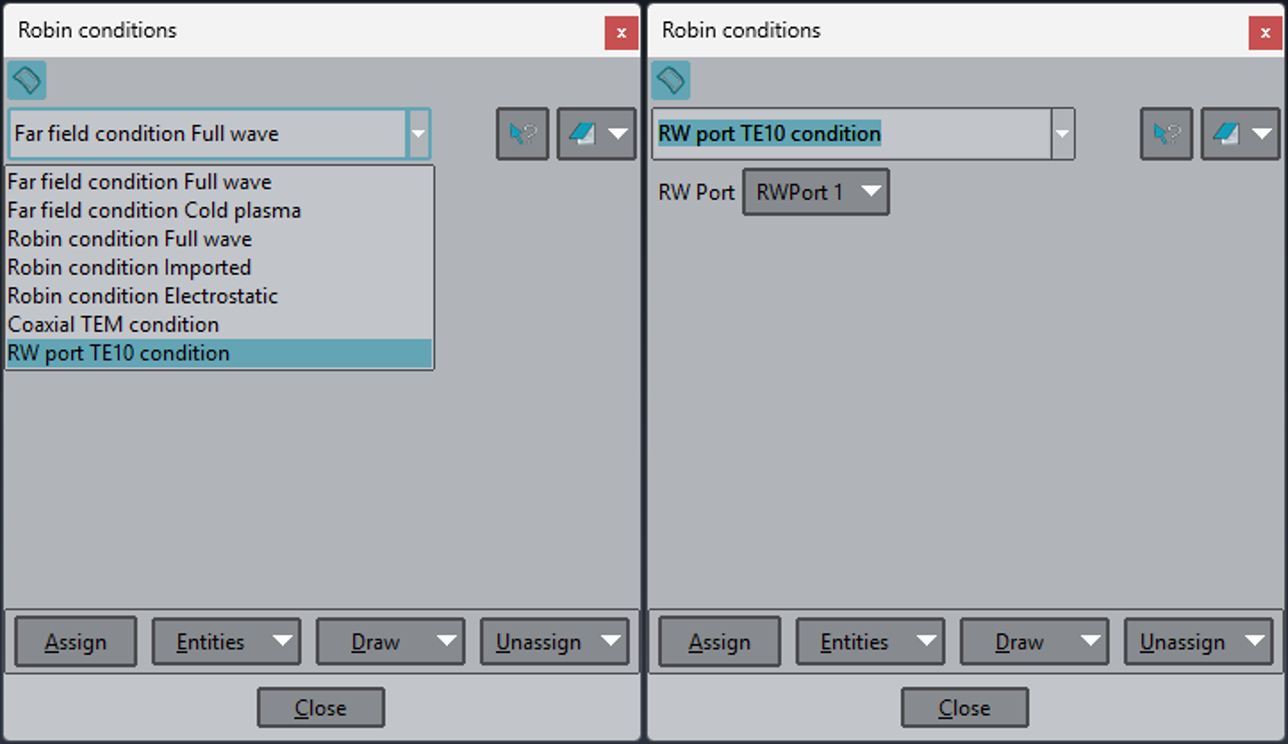
\includegraphics[width=0.78\textwidth]{Contents/Figures/Wins-Apply-RC.png}
		\caption{\textit{Robin conditions} window. This window can be accessed from the ERMES menu bar \ref{ERMES-MenuBar} by clicking the icon \textit{Robin boundary conditions}. From the drop-down menu, select the condition to apply. Next, choose the specific port, wave type, or current flux to assign.}\label{Wins-Apply-RC}
	\end{center}
\end{figure}

\begin{figure}[H]
	\begin{center}
		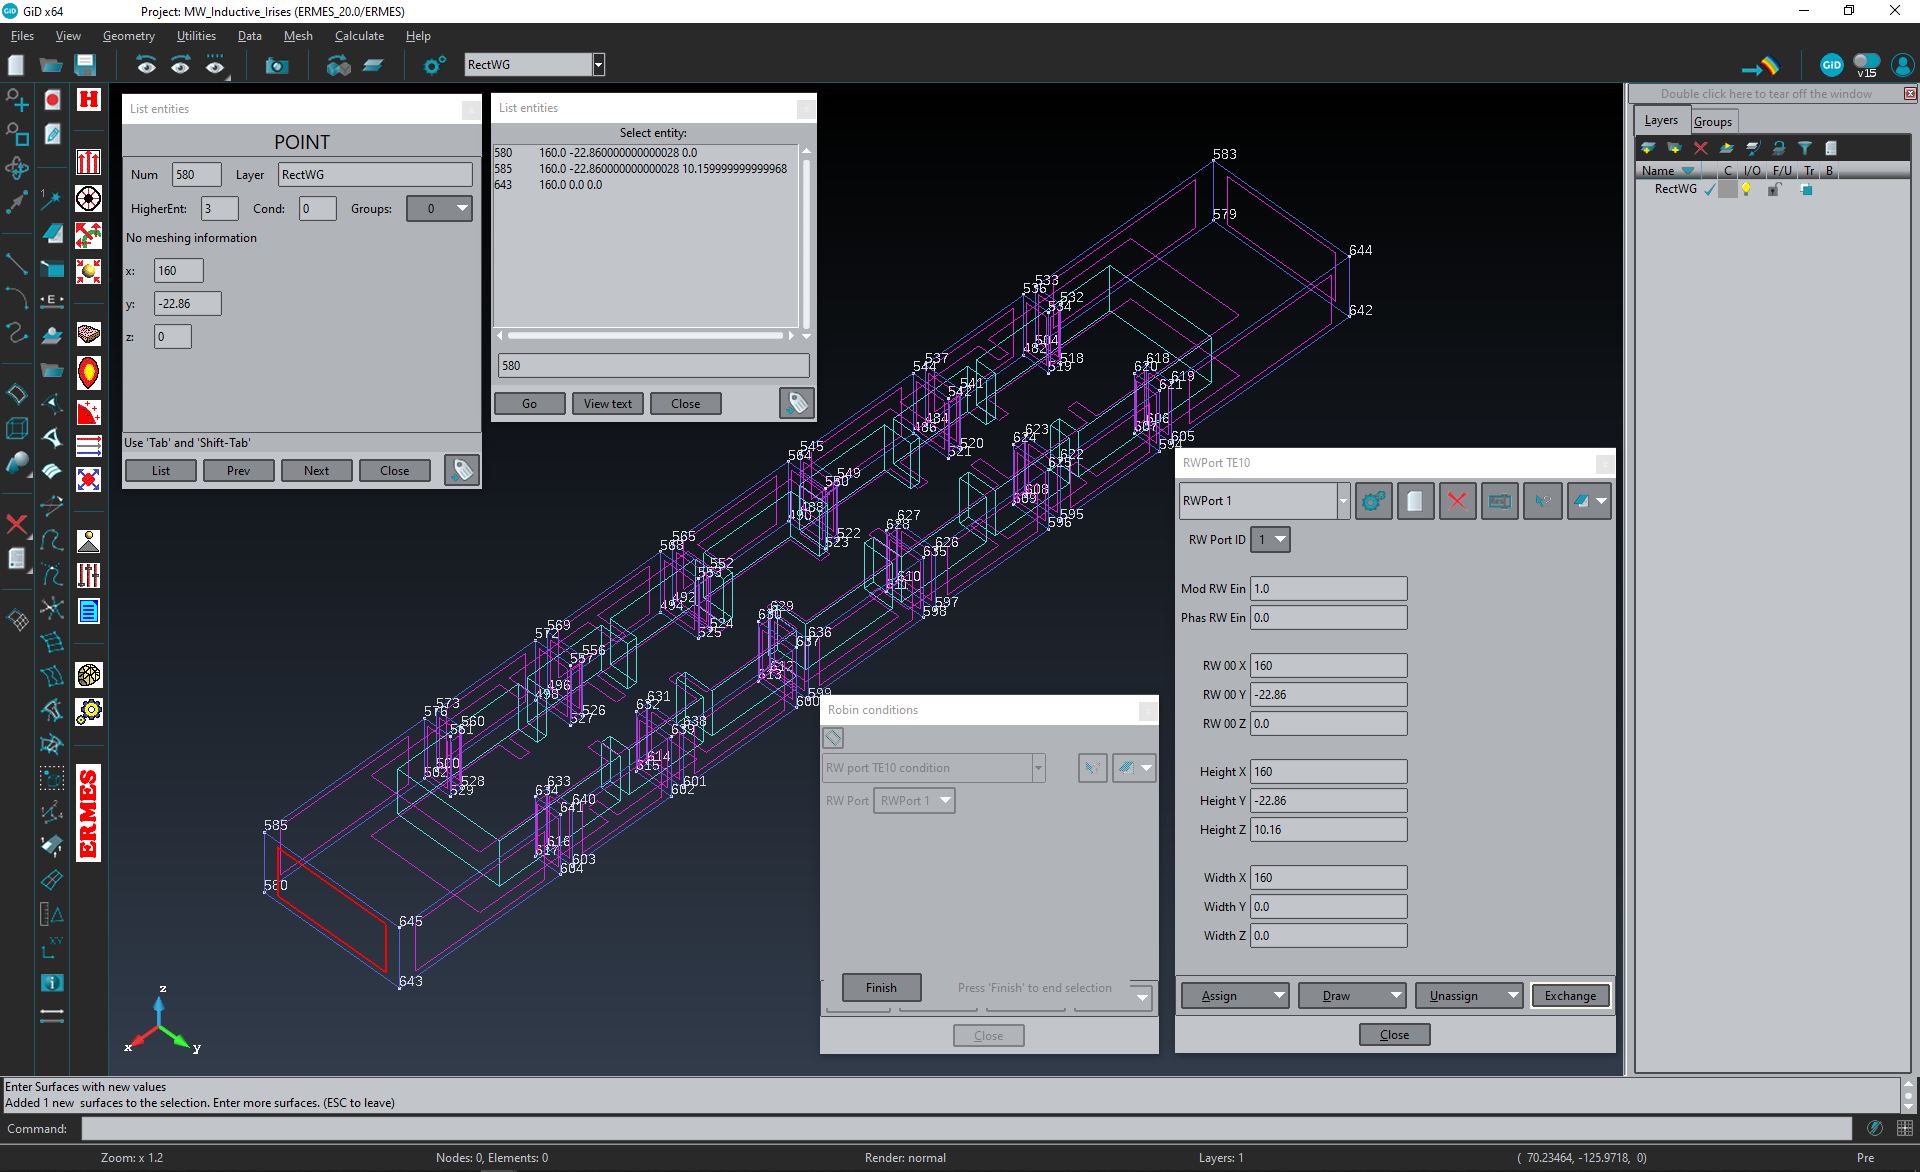
\includegraphics[width=0.95\textwidth]{Contents/Figures/AssignRWPort.png}
		\caption{From the \textit{Robin conditions} window \ref{Wins-Apply-RC}, click on the \textbf{\underline{A}ssign} button and select a surface. The surface will turn red as shown in the figure. Then, click on the central mouse button, the keyboard key \textit{Escape}, or the \textit{Finish} button to confirm the application.}\label{AssignRWPort}
	\end{center}
\end{figure}

\begin{figure}[H]
	\begin{center}
		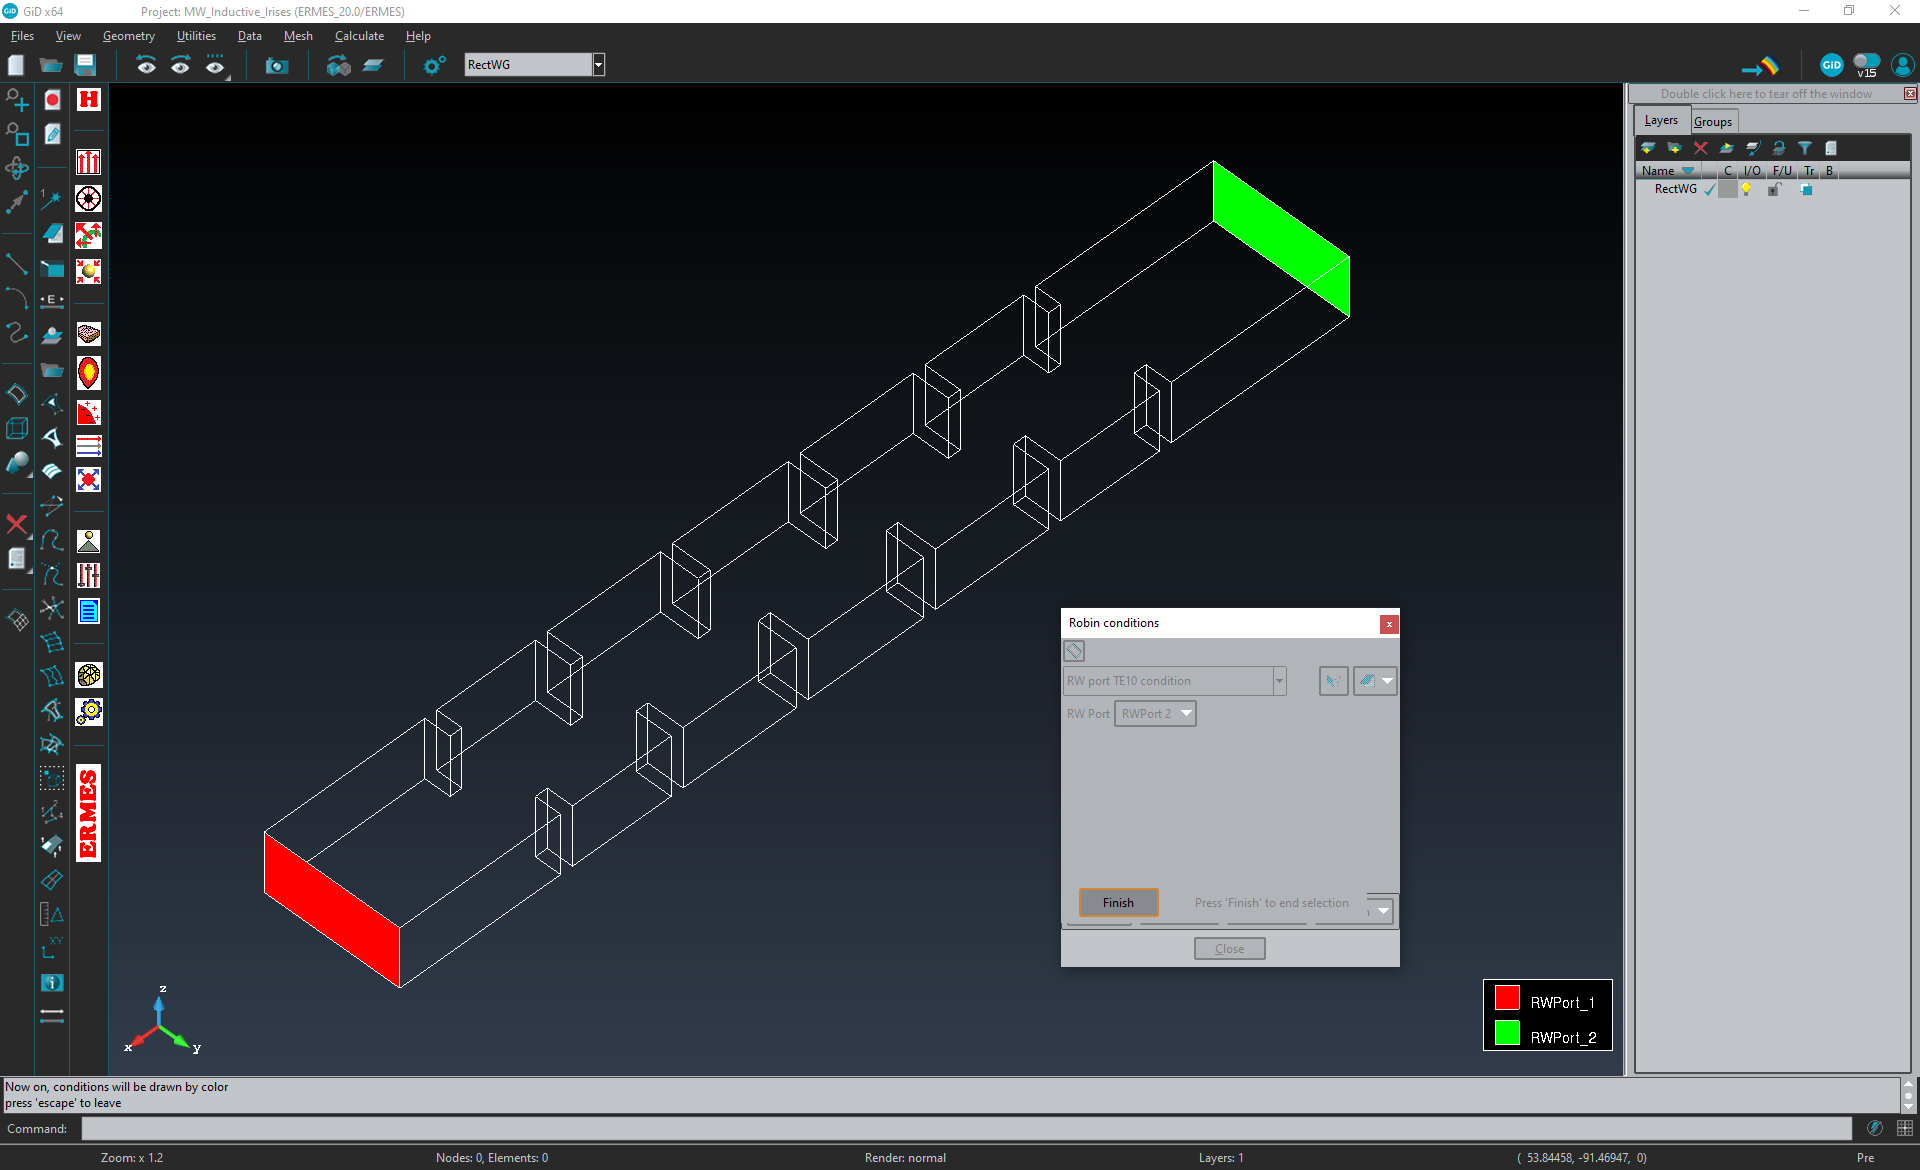
\includegraphics[width=0.95\textwidth]{Contents/Figures/CheckRWPort.png}
		\caption{To verify the correct application of the condition, navigate to the \textbf{\underline{D}raw} $\rightarrow$ \textbf{Colors} menu at the bottom of the \textit{Robin conditions} window \ref{Wins-Apply-RC}. If the condition has been correctly assigned, the selected surface will appear in a solid colour, along with other assigned Robin boundary conditions.}\label{CheckRWPort}
	\end{center}
\end{figure}

\subsubsection{Rectangular waveguide port - Figure \ref{Win-WG-Rect}}\label{bsRWPort}

The rectangular waveguide port boundary source assumes a transversal electromagnetic mode TE$_{10}$ at the port surface. The implemented electric field $\mathbf{E}_{10}$ of the fundamental mode $\text{TE}_{10}$ is:
\begin{equation}\label{E-TE10}
	\mathbf{E}_{10} = -|E_{0}|e^{i\theta}\sqrt{\frac{2i\omega\mu}{ab\gamma}}\,\sin(k_{c}x)\,e^{\gamma z}\,\mathbf{\hat{y}},
\end{equation}
where $|E_{0}|e^{i\theta}$ is a complex scale factor, $a$ is the width of the rectangular waveguide, $b$ is its height, $k_{c} = \pi / a$ and, $\gamma$ is the propagation constant of the mode $\text{TE}_{10}$, which is $\gamma = i\sqrt{k_{0}^2 - k_{c}^2}$ when $k_{0} > k_{c}$ and $\gamma = -\sqrt{k_{c}^2 - k_{0}^2}$ when $k_{0} < k_{c}$, being $k_{0} = \omega\sqrt{\epsilon_{0}\mu_{0}}$. In ERMES 20.0 the port surface can have any arbitrary orientation but, for clarity, in expression \eqref{E-TE10} is assumed that the x-axis is along the width of the rectangular waveguide, the y-axis is along its height and, the z-axis is perpendicular to the xy-plane, pointing inward to the waveguide volume. It is assumed z = 0 at the input port. For more information about rectangular waveguides, see references \cite{Pozar, Balanis}. 

The time-averaged input power $P_{0}$ of the TE$_{10}$ mode on the surface of the port is $P_{0} = |E_{0}|^2/2$, which allows the control of the input power with $|E_{0}|$. The port is assumed to be in vacuum and the parameters $|E_{0}|e^{i\theta}$, $\gamma$, $k_{c}$, $a$ and, $b$ are calculated from the information provided in the window \ref{Win-WG-Rect}:
\begin{itemize}\itemsep0em 
	\item \textbf{RW Port ID}: rectangular waveguide port identification number. This number is required for identifying the ports when calculating the $S_{ij}$ parameters. 
	\\
	\item \textbf{Mod RW Ein}: module of the complex scale factor $E_{0}$ multiplying the input TE$_{10}$ field. For an output port, use \textit{Mod RW Ein} = 0. For an input port, with a time-averaged input power equal to $P_{0}$,
	use \textit{Mod RW Ein} = $\sqrt{2P_{0}}$.
	\item \textbf{Phas RW Ein}: phase of the complex scale factor $E_{0}$ multiplying the input TE$_{10}$ field. For an output port, use \textit{Phas RW Ein} = 0. For an input port, with a phase equal to $\theta$ (rad), use \textit{Phas RW Ein} = $\theta$.
	\\
	\item \textbf{RW 00 X}: X coordinate of the lower left corner of the port.
	\item \textbf{RW 00 Y}: Y coordinate of the lower left corner of the port.
	\item \textbf{RW 00 Z}: Z coordinate of the lower left corner of the port.
	\\
	\item \textbf{Height X}: X coordinate of the upper left corner of the port.
	\item \textbf{Height Y}: Y coordinate of the upper left corner of the port.
	\item \textbf{Height Z}: Z coordinate of the upper left corner of the port.
	\\
	\item \textbf{Width X}: X coordinate of the lower right corner of the port.
	\item \textbf{Width Y}: Y coordinate of the lower right corner of the port.
	\item \textbf{Width Z}: Z coordinate of the lower right corner of the port.
\end{itemize}
where: 
\begin{equation}\label{RW-Parameters}
	\begin{aligned}\nonumber
	    |E_{0}| &= Mod\,RW\,Ein,\\
	    \theta\,\,\, &= Phas\,RW\,Ein,\\
	    a\,\,\, &= \sqrt{(Width\,\,X - RW\,00\,X)^2 + (Width\,\,Y - RW\,00\,Y)^2 + (Width\,\,Z - RW\,00\,Z)^2},\\
	    b\,\,\, &= \sqrt{(Height\,X - RW\,00\,X)^2 + (Height\,Y - RW\,00\,Y)^2 + (Height\,Z - RW\,00\,Z)^2}.\\
	\end{aligned}
\end{equation}
The mathematical expressions of the rectangular waveguide port boundary condition is:
\begin{equation}\label{RWRCExpanded}
	\mathbf{\hat{n}}\times\nabla\times\mathbf{E} - \gamma\,(\mathbf{\hat{n}}\times\mathbf{\hat{n}}\times\mathbf{E}) = -2\,\gamma\,(\mathbf{\hat{n}}\times\mathbf{\hat{n}}\times\mathbf{E}_{10}).
\end{equation}
This expression is properly tailored in ERMES 20.0 to suit the various FEM formulations implemented in it, as outlined in Appendix \ref{chFEMForms}. For the regularized and LL2P formulations, it is advisable to add a TEC Dirichlet condition \ref{ssDirichlet} ($\mathbf{\hat{n}}\cdot\mathbf{E} = 0$) on the port surfaces to enhance convergence.

\subsubsection{Coaxial waveguide port - Figure \ref{Win-WG-Coax}}\label{bsCoaxPort}

The coaxial waveguide port boundary source assumes a transversal electromagnetic mode TEM at the port surface. The implemented electric field $\mathbf{E}_{\text{TEM}}$ of the fundamental coaxial TEM mode is:
\begin{equation}\label{ETEM}
\mathbf{E}_{\text{TEM}} = |E_{0}|e^{i\theta}\sqrt{\frac{\eta}{2\pi\ln(b/a)}}\,\left(\frac{e^{\gamma\,z}}{\text{r}}\right)\,\mathbf{\hat{r}},
\end{equation}
where $|E_{0}|e^{i\theta}$ is a complex scale factor, $\eta = \sqrt{\mu/\varepsilon}$, $\gamma = i\omega\sqrt{\varepsilon\mu}$ is the propagation constant of the TEM mode, $a$ is the diameter of the inner cylinder of the coaxial waveguide, $b$ is the diameter of the exterior cylinder of the coaxial waveguide, $r$ is the radial coordinate $r = \sqrt{x^2 + y^2}$ and, $\mathbf{\hat{r}} = (x/r, y/r)$ is the unitary radial vector. In ERMES 20.0 the port surface can have any arbitrary orientation but, for clarity, the port plane in \eqref{ETEM} is assumed to be in the xy-plane and the direction of propagation is along the z-axis, pointing inward to the waveguide volume. It is assumed z = 0 at the input port. For more information about coaxial waveguides, see references \cite{Pozar, Balanis}. 

The time-averaged input power $P_{0}$ of the fundamental TEM mode \eqref{ETEM} is $P_{0} = |E_{0}|^2/2$, which allows the control of the input power with $|E_{0}|$. The port is assumed to be in a lossless IHL material and the parameters $|E_{0}|e^{i\theta}$, $\gamma$, $\eta$, $a$ and, $b$ are obtained from the information provided in the window \ref{Win-WG-Coax}:
\begin{itemize}\itemsep0em 
	\item \textbf{CC Port ID}: coaxial port identification number. This number is required for identifying the ports when calculating the $S_{ij}$ parameters. 
	\\
	\item \textbf{Mod CC Ein}: module of the complex scale factor $E_{0}$ multiplying the input TEM field. For an output port, use \textit{Mod CC Ein} = 0. For an input port, with a time-averaged input power equal to $P_{0}$,
	use \textit{Mod CC Ein} = $\sqrt{2P_{0}}$.
	\item \textbf{Phas CC Ein}: phase of the complex scale factor $E_{0}$ multiplying the input TEM field. For an output port, use \textit{Phas CC Ein} = 0. For an input port, with a phase equal to $\theta$ (rad), use \textit{Phas CC Ein} = $\theta$.
	\\
	\item \textbf{CC 00 X}: X coordinate of the centre of the coaxial waveguide port.
	\item \textbf{CC 00 Y}: Y coordinate of the centre of the coaxial waveguide port.
	\item \textbf{CC 00 Z}: Z coordinate of the centre of the coaxial waveguide port.
	\\
	\item \textbf{Inner D}: diameter of the inner cylinder of the coaxial waveguide.
	\item \textbf{Exter D}: diameter of the exterior cylinder of the coaxial waveguide.
	\\
	\item \textbf{Epr coax}: relative electric permittivity of the medium inside the coaxial waveguide.
	\item \textbf{Mu coax}: relative magnetic permeability of the medium inside the coaxial waveguide.
\end{itemize}
The mathematical expressions of the coaxial waveguide port boundary condition is:
\begin{equation}\label{CCRCExpanded}
	\mathbf{\hat{n}}\times\nabla\times\mathbf{E} - \gamma\,(\mathbf{\hat{n}}\times\mathbf{\hat{n}}\times\mathbf{E}) = -2\,\gamma\,(\mathbf{\hat{n}}\times\mathbf{\hat{n}}\times\mathbf{E}_{\text{TEM}}).
\end{equation}
This expression is properly tailored in ERMES 20.0 to suit the various FEM formulations implemented in it, as outlined in Appendix \ref{chFEMForms}. For the regularized and LL2P formulations, it is advisable to add a TEC Dirichlet condition \ref{ssDirichlet} ($\mathbf{\hat{n}}\cdot\mathbf{E} = 0$) on the port surfaces to enhance convergence.

\subsubsection{Plane waves - Figure \ref{Win-RC-PlaneWaves}}\label{bsPlaneWave}

The plane wave boundary source assumes a transversal plane wave at the boundary surface. The implemented electric field $\mathbf{E}_{\text{PW}}$ of the incident plane wave is:
\begin{equation}\label{EPW}
	\mathbf{E}_{\text{PW}} = |E_{0}|\,e^{i\theta}\,e^{\gamma\,\mathbf{\hat{k}}\cdot\mathbf{r}}\,\,\mathbf{\hat{e}}_{0},
\end{equation}
where $|E_{0}|e^{i\theta}$ is the complex amplitude of the plane wave, $\gamma = i\omega\sqrt{\varepsilon\mu}$ is the propagation constant, $\mathbf{\hat{k}}$ is the unit wave vector and, $\mathbf{\hat{e}}_{0}$ is the unit polarization vector. The parameters $|E_{0}|e^{i\theta}$, $\gamma$, $\mathbf{\hat{k}}$, and $\mathbf{\hat{e}}_{0}$ are derived from the information provided in the window \ref{Win-RC-PlaneWaves}:
\begin{itemize}\itemsep0em 
	\item \textbf{Multiple waves} [ \textbf{On} $\mid$ \textbf{Off} ]: enables the application of multiple plane waves on a boundary. All the plane waves with this option activated (\emph{Multiple waves} = \textit{On}) will be added coherently to the same boundary and with the same $\gamma$ as the assigned plane wave.
	\\
	\item \textbf{Module E field}: module of the plane wave complex amplitude ($|E_{0}|$).
	\item \textbf{Phase E field}: phase of the plane wave complex amplitude ($\theta$).
	\\
	\item \textbf{Polarization X}: X component of the polarization vector $\mathbf{\hat{e}}_{0}$.
	\item \textbf{Polarization Y}: Y component of the polarization vector $\mathbf{\hat{e}}_{0}$.
	\item \textbf{Polarization Z}: Z component of the polarization vector $\mathbf{\hat{e}}_{0}$.
	\\
	\item \textbf{Wave vector X}: X component of the wave vector $\mathbf{\hat{k}}$.
	\item \textbf{Wave vector Y}: Y component of the wave vector $\mathbf{\hat{k}}$.
	\item \textbf{Wave vector Z}: Z component of the wave vector $\mathbf{\hat{k}}$.
	\\
	\item \textbf{IBC conductivity real}: real part of the electric conductivity (S/m). 
	\item \textbf{IBC conductivity  img}: imaginary part of the electric conductivity (S/m). 
	\\
	\item \textbf{IBC permittivity real}: real part of the relative electric permittivity.
	\item \textbf{IBC permittivity  img}: imaginary part of the relative electric permittivity.
	\\
	\item \textbf{IBC permeability real}: real part of the relative magnetic permeability.
	\item \textbf{IBC permeability  img}: imaginary part of the relative magnetic permeability.
\end{itemize}
It is not necessary to provide the vectors \emph{Polarization XYZ} and \emph{Wave vector XYZ} normalized, as they are internally normalized within ERMES 20.0; however, they must be provided perpendicular to each other. The data entered in the IBC material properties fields should match the properties of the medium where the plane wave is incident. By setting \emph{Module E field} equal to zero ($|E_{0}| = 0$), the plane wave boundary condition can be used as an Impedance Boundary Condition (IBC) \eqref{ImperfectConductorE}. The mathematical expression of the plane wave boundary condition is:
\begin{equation}\label{PWRCExapanded}
	\mathbf{\hat{n}}\times\nabla\times\mathbf{E}\, - \,\gamma\,(\mathbf{\hat{n}}\times\mathbf{\hat{n}}\times\mathbf{E}) = - \,\gamma\,(\mathbf{\hat{n}}\times\mathbf{\hat{n}}\times\mathbf{E}_{\text{PW}})\, + \,\gamma\,(\mathbf{\hat{n}}\times\mathbf{\hat{k}}\times\mathbf{E}_{\text{PW}}),
\end{equation}
which differs slightly from the previous cases of rectangular and coaxial waveguides. The difference arises because the plane wave can be applied to curved domains, where the boundary normal is not necessarily parallel to the wave propagation vector of the incident field. The right-hand term of \eqref{PWRCExapanded} reduces to its equivalent \eqref{RWRCExpanded} or \eqref{CCRCExpanded} when $\mathbf{\hat{k}} = -\mathbf{\hat{n}}$, where $\mathbf{\hat{n}}$ is the unitary boundary normal pointing outward from the domain. For the regularized and LL2P formulations, the following extension of the divergence boundary condition is automatically applied inside ERMES 20.0:
\begin{equation}\label{PWRCDivExapanded}
	\nabla\cdot\mathbf{E} - \gamma\left(\mathbf{\hat{n}}\cdot\mathbf{E}\right) = -\,\gamma\, \mathbf{\hat{n}}\cdot\mathbf{E}_{\text{PW}}\, + \,\gamma\,\mathbf{\hat{k}}\cdot\mathbf{E}_{\text{PW}}
\end{equation}
In Appendix \ref{chFEMForms} can be consulted the adaptation of the above boundary conditions to all the different formulations implemented in ERMES 20.0.

\subsubsection{Gaussian beams - Figure \ref{Win-RC-GaussBeam}}\label{bsGaussBeam}

The Gaussian beam boundary source assumes the following electric field at the boundary:
\begin{equation}\label{EGB}
	\mathbf{E}_{\text{GB}} = \sqrt[4]{\frac{z_{\varrho}\,z_{\eta}}{|q_{\varrho}||\,q_{\eta}|}}\,\left[|E_{\varrho}|e^{i\theta_{\varrho}}\,\mathbf{\hat{\varrho}}\,\,+\,\,|E_{\eta}|e^{i\theta_{\eta}}\,\mathbf{\hat{\eta}}\right]e^{i\Phi}
\end{equation}
being:
\begin{equation}\label{EGB-zs}
    z_{\varrho} = \dfrac{k_{0}}{2}\,\,\omega^{2}_{\varrho}, \,\,\, z_{\eta} = \dfrac{k_{0}}{2}\,\,\omega^{2}_{\eta},
\end{equation}

\begin{equation}\label{EGB-qs}
	q_{\varrho} = \delta\,-\,iz_{\varrho}, \,\,\, q_{\eta} = \delta\,-\,iz_{\eta},
\end{equation}

\begin{equation}\label{EGB-Phi}
	\Phi = k_{0}\delta\,-\,\dfrac{1}{2}\left[\arctan\left(\frac{\delta}{z_{\varrho}}\right)\,+\,\arctan\left(\frac{\delta}{z_{\eta}}\right)\right]\,+\,\dfrac{k_{0}}{2}\left(\frac{\varrho^{2}}{q_{\varrho}}\,+\,\frac{\eta^{2}}{q_{\eta}}\right)
\end{equation}
where $|E_{\varrho}|e^{i\theta_{\varrho}}$ and $|E_{\eta}|e^{i\theta_{\eta}}$ are the transversal components of electric field at the beam waist centre, $k_{0} = \omega\sqrt{\epsilon_{0}\mu_{0}}$ is the angular wave number in vacuum, and $\omega_{\varrho}$ and $\omega_{\eta}$ are the semi-axis lengths of the elliptical cross-section of the beam at its waist. In expressions \eqref{EGB} to \eqref{EGB-Phi}, the origin of the coordinate system is placed at the centre of the beam waist. The $\varrho$- and $\eta$-axis are aligned with the principal axes of the elliptical cross-section of the beam, while the $\delta$-axis is aligned with the direction of propagation. The unit vectors $\mathbf{\hat{\varrho}}$, $\mathbf{\hat{\delta}}$, and $\mathbf{\hat{\eta}}$ satisfy the relations $\mathbf{\hat{\varrho}} \perp \mathbf{\hat{\delta}}$ and $\mathbf{\hat{\eta}} = \mathbf{\hat{\delta}} \times \mathbf{\hat{\varrho}}$. The unit vectors $\mathbf{\hat{\varrho}}$, $\mathbf{\hat{\eta}}$, and $\mathbf{\hat{\delta}}$, as well as the parameters $|E_{\varrho}|$, $\theta_{\varrho}$, $|E_{\eta}|$, $\theta_{\eta}$, $\omega_{\varrho}$, and $\omega_{\eta}$ are determined from the information provided in window \ref{Win-RC-GaussBeam}:
\begin{itemize}\itemsep0em 
	\item \textbf{GB module E par}: module of the electric field component $\mathbf{\hat{\varrho}}$ at the waist centre ($|E_{\varrho}|$).
	\item \textbf{GB phase E par}: phase of the electric field component $\mathbf{\hat{\varrho}}$ at the waist centre ($\theta_{\varrho}$).
	\\
	\item \textbf{GB module E per}: module of the electric field component $\mathbf{\hat{\eta}}$ at the waist centre ($|E_{\eta}|$).
	\item \textbf{GB phase E per}: phase of the electric field component $\mathbf{\hat{\eta}}$ at the waist centre ($\theta_{\eta}$).
	\\
	\item \textbf{GB radius par}: waist radius in the $\mathbf{\hat{\varrho}}$ direction ($\omega_{\varrho}$).
	\item \textbf{GB radius per}: waist radius in the $\mathbf{\hat{\eta}}$ direction ($\omega_{\eta}$).
	\\
	\item \textbf{GB 00 X}: X coordinate of the centre of the Gaussian beam waist.
	\item \textbf{GB 00 Y}: Y coordinate of the centre of the Gaussian beam waist.
	\item \textbf{GB 00 Z}: Z coordinate of the centre of the Gaussian beam waist.
	\\
	\item \textbf{GB polarization X}: X component of the polarization vector $\mathbf{\hat{\varrho}}$.
	\item \textbf{GB polarization Y}: Y component of the polarization vector $\mathbf{\hat{\varrho}}$.
	\item \textbf{GB polarization Z}: Z component of the polarization vector $\mathbf{\hat{\varrho}}$.
	\\
	\item \textbf{GB wave vector X}: X component of the wave propagation vector $\mathbf{\hat{\delta}}$.
    \item \textbf{GB wave vector Y}: Y component of the wave propagation vector $\mathbf{\hat{\delta}}$.
    \item \textbf{GB wave vector Z}: Z component of the wave propagation vector $\mathbf{\hat{\delta}}$.
\end{itemize}
It is not necessary to provide the vectors \emph{GB polarization XYZ} and \emph{GB wave vector XYZ} normalized, as they are internally normalized within ERMES 20.0; however, they must be provided perpendicular to each other. The mathematical form of the Gaussian beam boundary condition is:
\begin{equation}\label{GBRCExapanded}
	\mathbf{\hat{n}}\times\nabla\times\mathbf{E}\, - \,ik_{0}\,(\mathbf{\hat{n}}\times\mathbf{\hat{n}}\times\mathbf{E}) = - \,ik_{0}\,(\mathbf{\hat{n}}\times\mathbf{\hat{n}}\times\mathbf{E}_{\text{GB}})\, + \,ik_{0}\,(\mathbf{\hat{n}}\times\mathbf{\hat{\delta}}\times\mathbf{E}_{\text{GB}}),
\end{equation}
For the regularized and LL2P formulations, the following extension of the divergence boundary condition is automatically applied inside ERMES 20.0:
\begin{equation}\label{GBRCDivExapanded}
	\nabla\cdot\mathbf{E} - ik_{0}\left(\mathbf{\hat{n}}\cdot\mathbf{E}\right) = -\,ik_{0}\, \mathbf{\hat{n}}\cdot\mathbf{E}_{\text{GB}}\, + \,ik_{0}\,\mathbf{\hat{\delta}}\cdot\mathbf{E}_{\text{GB}}
\end{equation}
In Appendix \ref{chFEMForms} can be consulted the adaptation of the above boundary conditions to all the different formulations implemented in ERMES 20.0.

\begin{figure}[H]
	\begin{center}
		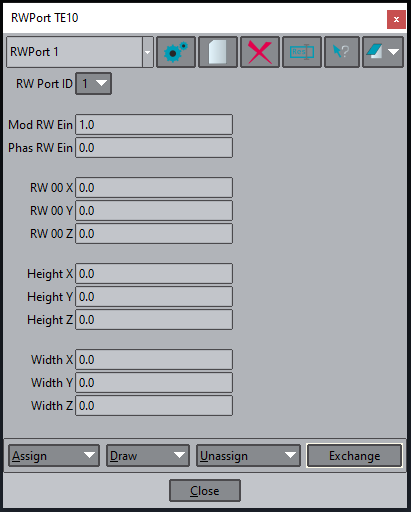
\includegraphics[width=0.45\textwidth]{Contents/Figures/Win-WG-Rect.png}
		\caption{Rectangular waveguide port properties window.}\label{Win-WG-Rect}
	\end{center}
\end{figure}

\begin{figure}[H]
	\begin{center}
		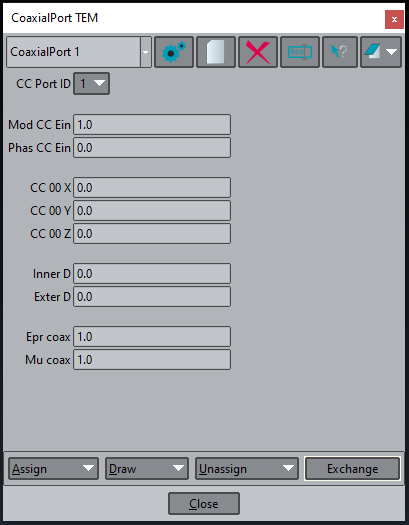
\includegraphics[width=0.45\textwidth]{Contents/Figures/Win-WG-Coax.png}
		\caption{Coaxial waveguide port properties window.}\label{Win-WG-Coax}
	\end{center}
\end{figure}

\begin{figure}[H]
	\begin{center}
		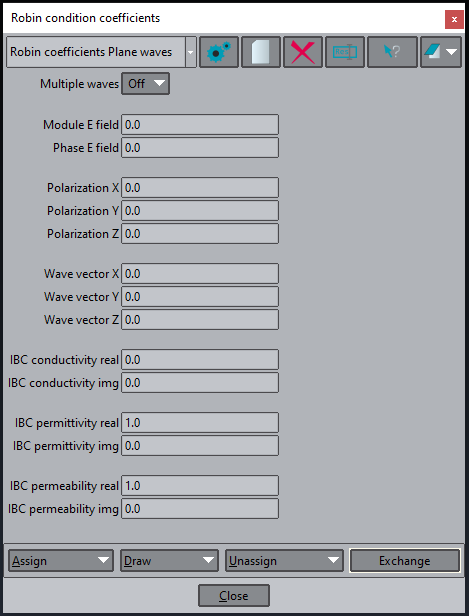
\includegraphics[width=0.43\textwidth]{Contents/Figures/Win-RC-PlaneWaves.png}
		\caption{Plane waves properties window.}\label{Win-RC-PlaneWaves}
	\end{center}
\end{figure}

\begin{figure}[H]
	\begin{center}
		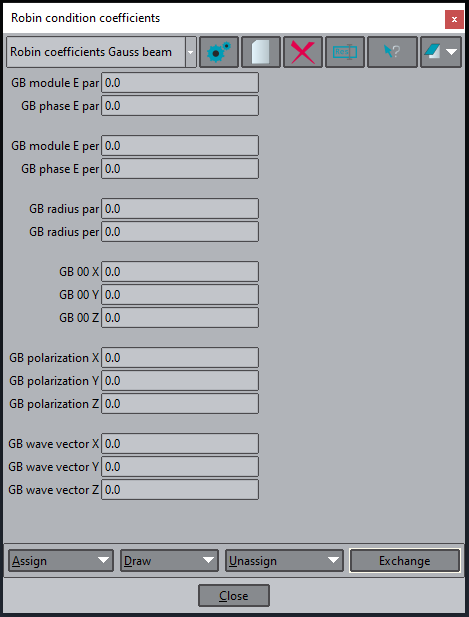
\includegraphics[width=0.43\textwidth]{Contents/Figures/Win-RC-GaussBeam.png}
		\caption{Gaussian beams properties window.}\label{Win-RC-GaussBeam}
	\end{center}
\end{figure}

\subsubsection{Quasi-static current flux - Figure \ref{Win-RC-Quasiestatic}}\label{bsRCQuasiStatic}

The quasi-static current flux source imposes a normal flux on the boundary through the following boundary condition: 
\begin{equation}\label{QSRCExapanded}
	\begin{aligned}
		\mathbf{\hat{n}}\times\nabla\times\mathbf{A} - \gamma(\mathbf{\hat{n}}\times\mathbf{\hat{n}}\times\mathbf{A}) &= \,\,\,0,
		\\
		\mathbf{\hat{n}}\cdot\omega^{2}\varepsilon\left(\mathbf{A} + \nabla\phi^{'}\right) &= \,|F_{n}|e^{i\theta_{n}},
	\end{aligned}
\end{equation}
where $\gamma$ is a complex number, and $|F_{n}|e^{i\theta_{n}}$ is the imposed normal flux. For the regularized and LL2P formulations, ERMES 20.0 automatically extends condition \eqref{QSRCExapanded} with the following divergence term (see Appendix \ref{chFEMForms}):
\begin{equation}
	\nabla\cdot\mathbf{A} - \gamma\left(\mathbf{\hat{n}}\cdot\mathbf{A}\right) = \,0.	
\end{equation}
The values of $\gamma$, $|F_{n}|$, and $\theta_{n}$ are obtained from the data provided in window \ref{Win-RC-Quasiestatic}:
\begin{itemize}\itemsep0em 
	\item \textbf{Robin coeff real}: real part of $\gamma$. 
	\item \textbf{Robin coeff  img}: imaginary part of $\gamma$. 
	\item \textbf{Module Flux}: module of the imposed normal flux ($|F_{n}|$).
	\item \textbf{Phase Flux}: phase of the imposed normal flux ($\theta_{n}$).
\end{itemize}
This boundary source is specifically designed for the $\textbf{A}-\phi$ potentials formulations (see Appendix \ref{chFEMForms}). It is particularly effective at low frequencies when $\omega^{2}\varepsilon \approx i\omega\sigma^{'}$ or, equivalently, $\sigma^{'} \gg \epsilon^{'}\omega$ (assuming $\sigma^{''}$ and $\epsilon^{''}$ equal to zero, see definition \eqref{ComplexPermittivityIHL}). Under these conditions, with $\gamma = 0$, the boundary source \eqref{QSRCExapanded} directly imposes a normal current density $J_{n} = |F_{n}|e^{i\theta_{n}}$ on the boundary. This result follows from applying the approximation $\omega^{2}\varepsilon \approx i\omega\sigma^{'}$ in \eqref{QSRCExapanded} and the fact that, in the $\textbf{A}-\phi$ potentials formulations, $\mathbf{E} = i\omega(\mathbf{A} + \nabla\phi^{'})$ and $\mathbf{J} = \sigma^{'}\mathbf{E}$. 

Additionally, condition \eqref{QSRCExapanded} can also be used as a generic Robin boundary condition when $\gamma \neq 0$. As an example, it can be used to impose a quasi-static far-field condition on a boundary with a curvature radius $\rho$. This is achieved by setting $|F_{n}| = 0$ and defining the parameter $\gamma$ as: 
\begin{equation}
	\gamma = \frac{1}{\rho\mu_{0}}.	
\end{equation}

\subsubsection{Electrostatic current flux - Figure \ref{Win-RC-Electrostatic}}\label{bsRCElectroStatic}

The electrostatic current flux source imposes a normal flux on the boundary through the following boundary condition: 
\begin{equation}\label{ESRCExapanded}
	\mathbf{\hat{n}}\cdot\left(\eta\nabla\phi\right) + \gamma\phi = q,
\end{equation}
where $\eta = \sigma^{'}$ when $\sigma^{'} > 0$ in the domain, and $\eta = \epsilon^{'}$ otherwise. The coefficients $\gamma$ and $q$ are real numbers obtained from the data provided in window \ref{Win-RC-Electrostatic}:
\begin{itemize}\itemsep0em 
	\item \textbf{Robin coeff}: Robin coefficient $\gamma$.
	\item \textbf{Flux}: Robin flux $q$.
\end{itemize}
This boundary source is only defined when the \textit{Electrostatic} mode is activated (see Section \ref{ProblemSettings}). In \textit{Electrostatic} mode, ERMES 20.0 solves the equation:
\begin{equation}\label{Laplace}
	- \nabla\cdot\left(\eta\nabla\phi\right) = 0.
\end{equation}
Recalling that in electrostatics, $\mathbf{E} = -\nabla\phi$, the equation is equivalent to $\nabla\cdot\mathbf{D} = 0$ or $\nabla\cdot\mathbf{J} = 0$, depending on whether $\eta = \epsilon^{'}$ or $\eta = \sigma^{'}$, respectively.

The boundary condition \eqref{ESRCExapanded} can be used to inject a current density $q$ into  the domain by setting $\gamma = 0$, or as a far-field electrostatic condition by setting $q = 0$ and $\gamma = 1/\rho$, where 
$\rho$ is the radius of curvature of the domain.
\quad\\

\begin{figure}[H]
	\begin{center}
		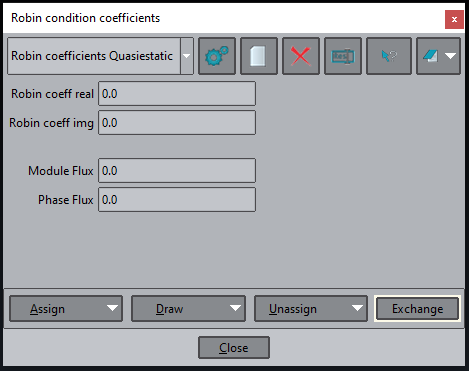
\includegraphics[width=0.5\textwidth]{Contents/Figures/Win-RC-Quasiestatic.png}
		\caption{Current flux properties window for quasi-statics.}\label{Win-RC-Quasiestatic}
	\end{center}
\end{figure}

\begin{figure}[H]
	\begin{center}
		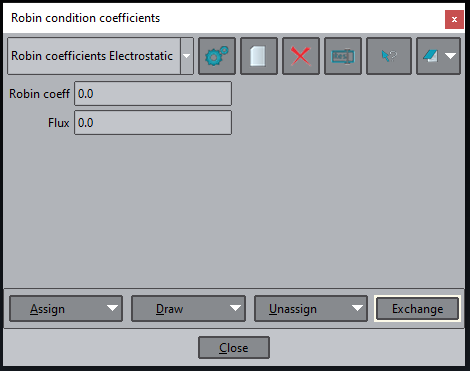
\includegraphics[width=0.5\textwidth]{Contents/Figures/Win-RC-Electrostatic.png}
		\caption{Current flux properties window for electrostatics.}\label{Win-RC-Electrostatic}
	\end{center}
\end{figure}

\section{Boundary conditions}

In ERMES 20.0, two types of boundary conditions are available:
\begin{itemize}\itemsep0em 
	\item Dirichlet boundary conditions,
	\item Robin boundary conditions.
\end{itemize}
Dirichlet boundary conditions impose constraints on the field values, while Robin boundary conditions impose constrains on the derivatives of the fields. This section provides a detailed explanation of all the available boundary conditions.

\subsection{Dirichlet boundary conditions}\label{ssDirichlet}

The Dirichlet boundary conditions window \ref{Win-DC-DropDown} can be accessed by clicking on the \textit{Dirichlet boundary conditions} icon in the ERMES menu bar \ref{ERMES-MenuBar}:
\quad\\

\begin{figure}[H]
	\begin{center}
		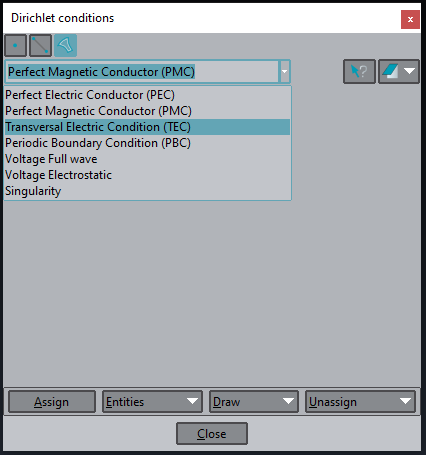
\includegraphics[width=0.45\textwidth]{Contents/Figures/Win-DC-DropDown.png}
		\caption{Dirichlet boundary conditions window.}\label{Win-DC-DropDown}
	\end{center}
\end{figure}

\noindent In ERMES 20.0, Dirichlet conditions can be assigned to points, lines, and surfaces. The desired geometric object can be selected by choosing one of the icons in the upper-left corner of \ref{Win-DC-DropDown}. Once the geometric object to which the condition will be applied is chosen, the appropriate boundary condition for that object must be selected. After selecting the condition, any additional options (which will be explained in the following) should be configured. Finally, the boundary condition is assigned to a point, line, or surface following a procedure similar to that illustrated in Figures \ref{AssignRWPort} and \ref{CheckRWPort}, using the \textbf{\underline{A}ssign} button located in the lower-left corner of the Dirichlet boundary conditions window \ref{Win-DC-DropDown}. The available Dirichlet conditions are the following:

\begin{itemize}\itemsep0em\label{DirichletBCExp} 
	\item \textbf{Perfect Electric Conductor (PEC)} - [ \textit{Surfaces} ]:\\ 
	For $\mathbf{E}$-field formulations, it imposes $\mathbf{\hat{n}}\times\mathbf{E} = 0$ on the surface. For $\mathbf{A}-\phi$ potential formulations, it sets $\mathbf{\hat{n}}\times\mathbf{A} = 0$ and $\phi = 0$ on the surface. For edge-stabilized formulations, it additionally sets the Lagrange multiplier $\varphi$ equal to zero on the surface.
	\\
	\item \textbf{Perfect Magnetic Conductor (PMC)} - [ \textit{Surfaces} ]:\\ 
	For regularized and LL2P $\mathbf{E}$-field formulations, it imposes $\mathbf{\hat{n}}\cdot\mathbf{E} = 0$ on the surface. For regularized and LL2P $\mathbf{A}-\phi$ potential formulations, it sets $\mathbf{\hat{n}}\cdot\mathbf{A} = 0$ on the surface. It is redundant for double-curl edge formulations. This condition is specifically designed for symmetry surfaces.
	\\
	\item \textbf{Transversal Electric Condition (TEC)} - [ \textit{Surfaces} ]:\\ 
	For regularized and LL2P $\mathbf{E}$-field formulations, it imposes $\mathbf{\hat{n}}\cdot\mathbf{E} = 0$ on the surface. For regularized and LL2P $\mathbf{A}-\phi$ potential formulations, it sets $\mathbf{\hat{n}}\cdot\mathbf{A} = 0$ on the surface. It is redundant for double-curl edge formulations. This condition is specifically designed for waveguide port surfaces. 
	\\
	\item \textbf{Periodic Boundary Condition (PBC)} - [ \textit{Surfaces} ]:\\ 
    It enforces equal fields with a specified phase difference on two separate surfaces. It can also be used to impose cyclic boundary conditions. The PBC type (periodic or cyclic) and the phase difference between the two surfaces must be specified in the \textbf{Geometry} tab of the \textbf{Solving parameters} window \ref{Win-PSettings-2}.
    
    To apply a PBC, the two surfaces must have identical meshes. To generate identical meshes on two separate surfaces, click \textbf{\underline{G}eometry} $\rightarrow$ \textbf{Create} $\rightarrow$ \textbf{Contact} $\rightarrow$ \textbf{Separated Volume} in the GiD upper menu, and then select the two surfaces. GiD will generate identical triangular meshes on both surfaces by connecting the corresponding triangles with prismatic contact elements. 
    
    These contact elements are not required for the PBCs. If they are retained, ERMES 20.0 will treat the corresponding surfaces as a field discontinuity (see Section~\ref{Discontinuities}). If the materials on both surfaces are the same, the discontinuity matrix \eqref{DobleNodeMatrix} is reduced to the identity matrix, thereby enforcing equal field values on the corresponding nodes of the opposing surfaces.
    
    To avoid the application of the discontinuity matrix \eqref{DobleNodeMatrix}, the contact elements must be disabled by selecting \textbf{\underline{M}esh} $\rightarrow$ \textbf{Mesh Criteria} $\rightarrow$ \textbf{No Mesh} $\rightarrow$ \textbf{Volumes} from the GiD upper menu, and then selecting the contact volume, which is displayed as a blue arrow connecting the two surfaces. \textbf{Disabling the meshing of the contact volume prevents the creation of contact elements while preserving identical meshes on the two surfaces.}
    
    An alternative way to neglect the contact volume mesh is to select the \textbf{Ignore} option for the \textbf{Contact detect} setting in the \textbf{Solving parameters} $\rightarrow$ \textbf{Geometry} window \ref{Win-PSettings-2}. This option causes ERMES 20.0 to ignore all contact volumes defined in the geometry, including those intended to represent field discontinuities. Therefore, it should only be used when none of the contact volumes are required to model discontinuities. If field discontinuities are included in the model, the \textbf{Manual} option must be selected in \textbf{Contact detect}, and the contact volumes used for the PBCs must be explicitly set as volumes not to be meshed, as indicated in the previous paragraph.
    
    Anyhow, if PBCs are required only between parallel surfaces (i.e., periodic PBCs) with no phase difference, contact volume elements can be used as an equivalent alternative for both edge and nodal element formulations. Furthermore, for edge elements, contact volume elements can also be used interchangeably for cyclic and periodic PBCs, provided that no phase difference exists between the paired surfaces. In contrast, for nodal elements, cyclic PBCs cannot be implemented using contact elements; therefore, the PBCs must be applied explicitly in this case.
    
    There are two pairs of PBC surfaces: \textbf{Front}-\textbf{Back} and \textbf{Right}-\textbf{Left}. The \textbf{Front}-\textbf{Back} surfaces must always lie parallel to the XY-plane. For cyclic PBCs, the \textbf{Left} surface must lie in the YZ-plane, and the axis of rotation must be the Z-axis.
    
    The \textbf{Front} and \textbf{Right} surfaces are defined as slave surfaces, while the \textbf{Back} and \textbf{Left} surfaces act as master surfaces. This means that the fields are computed using the master surfaces, and the values on the slave surfaces are then expressed as a function of the master surfaces fields after the global linear system has been solved, according to
    \begin{equation}\label{EPBCs}
	    \begin{aligned}
		    \mathbf{E}_f &= \,\mathbf{E}_b \,\, e^{i(\Psi_f - \Psi_b)}, 
		    \\
		    \mathbf{E}_r &= \,\mathbf{E}_l \,\, e^{i(\Psi_r - \Psi_l)},
	    \end{aligned}
    \end{equation}
    where the subscripts $f$, $b$, $r$, and $l$ refer to the front, back, right, and left surfaces, respectively, and $\Psi$ denotes the phase of the fields on each surface. For the $\mathbf{A}-\phi$ potential formulation, the phase difference is applied to both the vector potential $\mathbf{A}$ and the scalar potential $\phi$.
    \\
	\item \textbf{Voltage Full wave} - [ \textit{Points $\mid$ Lines $\mid$ Surfaces} ]:\\ 
	It imposes a time-harmonic voltage $|V_{0}|e^{i\theta_{0}}$ on a point, line, or surface. It is defined for the \textit{Full wave} and \textit{Cold plasma} modes.
    \\
	\item \textbf{Voltage Electrostatic} - [ \textit{Points $\mid$ Lines $\mid$ Surfaces} ]:\\
	It imposes a electrostatic voltage $V_{0}$ on a point, line, or surface. It is defined for the \textit{Electrostatic} mode.
	\\
	\item \textbf{Singularity} - [ \textit{Points $\mid$ Lines $\mid$ Surfaces} ]:\\
	It sets the number of ungauged layers around a point, line, or surface (see Section \ref{Singularities}). In the regularized formulations, the divergence term of the elements inside the ungauged layers is removed. In the LL2P formulations, both the divergence term and the bubble contribution of the elements inside the ungauged layers are removed.
\end{itemize}

\subsection{Robin boundary conditions}

The Robin boundary conditions window \ref{Wins-Apply-RC} can be accessed by clicking on the \textit{Robin boundary conditions} icon in the ERMES menu bar \ref{ERMES-MenuBar}. In ERMES 20.0, Robin conditions can only be assigned to surfaces. Section \ref{ssBoundarySources} explains how to assign Robin boundary conditions to surfaces and how to define their coefficients. The following Robin conditions are available in ERMES 20.0:
\begin{itemize}\itemsep0em 
	\item \textbf{Far field condition Full wave} - [ \textit{Surfaces} ]:\\ 
	It applies the following time-harmonic far-field condition to a boundary placed in vacuum:
	\begin{equation}\label{FFVBC}
		\mathbf{\hat{n}}\times\nabla\times\mathbf{E}\, - \,i\omega\sqrt{\epsilon_{0}\mu_{0}}\,\left(\mathbf{\hat{n}}\times\mathbf{\hat{n}}\times\mathbf{E}\right) = 0.
	\end{equation}
	Appendix \ref{chFEMForms} describes the adaptation of \eqref{FFVBC} to the various FEM formulations implemented in ERMES 20.0.
    \\
	\item \textbf{Far field condition Cold plasma} - [ \textit{Surfaces} ]:\\ 
	It applies the following time-harmonic far-field condition to a boundary enclosing a cold plasma:
	\begin{equation}\label{FFCPBC}
		\mathbf{\hat{n}}\times\nabla\times\mathbf{E}\, - \,ik_{cp}\,\left(\mathbf{\hat{n}}\times\mathbf{\hat{n}}\times\mathbf{E}\right) = 0,
	\end{equation}
	where $k_{cp} = \omega\sqrt{\eta\,\epsilon_{0}\mu_{0}}$, with $\eta$ being a position-dependent parameter calculated within ERMES 20.0. The parameter $\eta$ can have different values depending on the type of cold plasma wave applied to the boundary. There are four possible choices:
	\begin{itemize}\itemsep0em 
		\item \textbf{FW}: $\eta = RL/S$ (extraordinary wave).
		\item \textbf{RW}: $\eta = R$ (right-handed polarized wave).
		\item \textbf{LW}: $\eta = L$ (left-handed polarized wave).
		\item \textbf{PW}: $\eta = P$ (ordinary wave).
	\end{itemize}
	where $R$, $L$, $S$, and $P$ are components of the cold plasma permittivity tensor \cite{Stix, Swanson}. If \eqref{FFCPBC} is applied in vacuum, it becomes equal to \eqref{FFVBC}. Appendix \ref{chFEMForms} shows the adaptation of \eqref{FFCPBC} to the various FEM formulations implemented in ERMES 20.0.
    \\
	\item \textbf{Robin condition Full wave} - [ \textit{Surfaces} ]:\\
	It applies a Robin boundary condition using the coefficients defined in:	
	\begin{itemize}\itemsep0em 
	    \item \textbf{Robin coefficients Plane waves} \ref{bsPlaneWave} - \ref{Win-RC-PlaneWaves}.
	    \item \textbf{Robin coefficients Gauss beam} \ref{bsGaussBeam} - \ref{Win-RC-GaussBeam}.
	    \item \textbf{Robin coefficients Quasiestatic} \ref{bsRCQuasiStatic} - \ref{Win-RC-Quasiestatic}.\\
    \end{itemize}
    \item \textbf{Robin condition Imported} - [ \textit{Surfaces} ]:\\
    It applies the following generic Robin boundary condition \cite{JinAntArr}:
    \begin{equation}\label{IRBC}
    	\mathbf{\hat{n}}\times\nabla\times\mathbf{E}\, + \,P(\mathbf{E}) = \mathbf{U},
    \end{equation}
    where $P(\mathbf{E})$ and $\mathbf{U}$ are computed externally and subsequently imported into ERMES 20.0 from the files \path{Vector_U_IRBC.bin} and \path{Matrix_P_IRBC.bin}. These files must be located in the problem directory. An example illustrating both their generation and required format is provided in the problemtype folder \path{\Documents\Import_Scripts}. This boundary condition extends the capabilities of ERMES 20.0 by enabling multimode waveguide conditions \cite{JinAntArr}, incorporating spatial Fourier transforms for coupling with other codes, and supporting advanced techniques such as domain decomposition methods.
    \\
	\item \textbf{Robin condition Electrostatic} - [ \textit{Surfaces} ]:\\
	It applies a Robin boundary condition using the coefficients defined in \textit{Robin coefficients Electrostatic} \ref{bsRCElectroStatic} - \ref{Win-RC-Electrostatic}.
    \\
	\item \textbf{Coaxial TEM condition} - [ \textit{Surfaces} ]:\\
	It applies a Robin boundary condition using the coefficients defined in \textit{CoaxialPort TEM} \ref{bsCoaxPort} - \ref{Win-WG-Coax}.
	\\
	\item \textbf{RW port TE10 condition} - [ \textit{Surfaces} ]:\\
	It applies a Robin boundary condition using the coefficients defined in \textit{RWPort TE10} \ref{bsRWPort} - \ref{Win-WG-Rect}.
\end{itemize}

\section{Problem settings}\label{ProblemSettings}

Problem parameters such as frequency, FEM formulation, and solver type are set in the \textit{Solving parameters} window, which can be accessed via the icon of the same name on the ERMES menu bar \ref{ERMES-MenuBar}. The \textit{Solving parameters} window is divided into the five tabs shown in Figures \ref{Win-PSettings-1} to \ref{Win-PSettings-5}. A detailed description of each parameter within each tab is provided below.

\subsubsection{FEM formulation - Figure \ref{Win-PSettings-1}}\label{GeneralSettings}

\begin{itemize}\itemsep0em 
	\item \textbf{Problem mode}: the available problem modes are:
	\begin{itemize}\itemsep0.25em 
		\item \textbf{Full wave}: for solving problems in frequency domain with IHL materials.
		\item \textbf{Electrostatic}: for solving electrostatic problems.
		\item \textbf{Cold plasma}: for solving time-harmonic problems with a cold plasma.
    \end{itemize}
    \quad
	\item \textbf{Symmetry}: symmetry conditions applied to the main field across the entire problem domain. The main field can be either \textbf{E} or \textbf{A}, depending on the selected FEM formulation. Available options are: 
	\begin{itemize}\itemsep0.5em 
		\item \textbf{3D}: for solving a general three-dimensional problem.
		\item \textbf{XY}: for solving only the X- and Y-components of the main field, while setting the Z-component to zero throughout the entire domain. This symmetry is only available in \textit{Full wave} mode and is not supported for edge element formulations.
		\item \textbf{ZZ}: for solving only the Z-component of the main field, while setting the X- and Y-component to zero throughout the entire domain. The main field is set to zero on all PEC surfaces. This symmetry is only available in \textit{Full wave} mode and is not supported for edge element formulations.
		\item \textbf{AY}: for solving an axisymmetric problem around the Y axis, with the $\theta$- and r-components of the main field set to zero throughout the entire domain. The main field is set to zero on all PEC surfaces. This symmetry is only available in \textit{Full wave} mode and is not supported for edge element formulations.
	\end{itemize}
    \quad
	\item \textbf{Element type}: this setting specifies the FEM formulation and the element order to be used in that formulation (see Appendix \ref{chFEMForms}):
	\begin{itemize}\itemsep0.25em 
		\item \textbf{EDG 1st}\,\,: double-curl edge formulation with 1st order elements \ref{DoubleCurlEdge}.
		\item \textbf{EDG 2nd}: double-curl edge formulation with 2nd order elements \ref{DoubleCurlEdge}.
		\item \textbf{RME 1st}\,\,: regularized Maxwell equations method with 1st order nodal elements \ref{RMENodal}.
		\item \textbf{RME 2nd}: regularized Maxwell equations method with 2nd order nodal elements \ref{RMENodal}.
		\item \textbf{LL2P 3sb}: local $\text{L}^{2}$ projection method with 1st order nodal elements enriched with three surface bubbles plus an inner volumetric bubble \ref{LL2PNodalBubb}.
	\end{itemize}
	\quad
	\item \textbf{Potentials}: it selects between two different versions of the chosen FEM formulation:
	\begin{itemize}\itemsep0.25em 
		\item \textbf{On }: the problem is solved using the $\textbf{A}-\phi$ potentials version: \ref{sEdgePotentials}, \ref{RMEPotentials}, \ref{LL2PPotentials}.
		\item \textbf{Off}: the problem is solved using the $\textbf{E}$-field version: \ref{DoubleCurlEdge}, \ref{RMENodal}, \ref{LL2PNodalBubb}.
	\end{itemize}
	\quad
	\item \textbf{RME stabilize}: it maintains or removes the divergence term throughout the entire domain in the regularized \ref{RMENodal} and LL2P \ref{LL2PNodalBubb} formulations:
	\begin{itemize}\itemsep0.25em 
		\item \textbf{On }: maintains the divergence term.
		\item \textbf{Off}: removes the divergence term throughout the entire domain.
	\end{itemize}
	\quad
	\item \textbf{EDG stabilize}: it adds a stabilization term to the double-curl formulation \ref{DoubleCurlEdge}:
	\begin{itemize}\itemsep0.25em 
		\item \textbf{On }: the problem is solved with the stabilized term \ref{EdgeDoubleCurlStab}.
		\item \textbf{Off}: the problem is solved without the stabilization term \ref{DoubleCurlEdge}-\ref{sEdgePotentials}.
	\end{itemize}
	\quad
	\item \textbf{LL2P stabilize}: it adds a stabilization term to the LL2P formulation \ref{LL2PNodalBubb}:
	\begin{itemize}\itemsep0.25em 
		\item \textbf{On }: the problem is solved with the stabilized term \ref{LL2PStab} with $h_{k} = 1$.
		\item \textbf{Off}: the problem is solved without the stabilization term \ref{LL2PNodalBubb}-\ref{LL2PPotentials}.
	\end{itemize}
	\quad
	\item \textbf{Results mode}: it selects between three different results visualization modes:
	\begin{itemize}\itemsep0.25em 
		\item \textbf{Nodes}: the results are given at the nodes.
		\item \textbf{GP 1}: the results are given at the central Gauss points of the elements.
		\item \textbf{GP 4}: the results are given at four internal Gauss points of the elements.
	\end{itemize}
	\quad
	\item \textbf{LL2P smooth}: it smooths the solution of the LL2P method. This option is useful for mitigating numerical oscillations that can arise because of oversampling when using bubble elements:
	\begin{itemize}\itemsep0.25em 
		\item \textbf{On }: the smoothing is applied to the LL2P solution.
		\item \textbf{Off}: the smoothing is not applied to the LL2P solution.
	\end{itemize}
	\quad
	\item \textbf{Solving mode}: it selects between three different solving modes:
	\begin{itemize}\itemsep0.5em 
		\item \textbf{Release}: the problem is solved normally.
		\item \textbf{Debug}: the problem is not solved, but some results are generated for debugging purposes. This option is useful for verifying that the cold plasma is properly set up or ensuring that the contact elements are well defined.
		\item \textbf{Read}: the problem is not solved, but new results are generated after reading the \path{Vector_Xo.bin} file calculated previously. This option will create a new results file and is useful for adding results that were previously overlooked.
	\end{itemize}
\end{itemize}

\subsubsection{Geometry settings - Figure \ref{Win-PSettings-2}}

\begin{itemize}\itemsep0.25em 
	\item \textbf{Length units}: a multiplicative factor applied to all length values.
	\quad
	\item \textbf{Geo error tol}: error tolerance for GiD geometric objects. This setting can help ensure accurate axis alignment in axisymmetric simulations.
	\quad
	\item \textbf{Normals type}: criteria for computing the normals on PEC, PMC, and contact surfaces:
    \begin{itemize}\itemsep0em 
	    \item \textbf{Area weighted}: normals are calculated using a surface-weighted average.
	    \item \textbf{Geometric average}: normals are calculated as the average of the surrounding element normals, ignoring their relative sizes.
    \end{itemize}	
    \quad
	\item \textbf{AV continuity}: allows for continuous or discontinuous normal components of the vector potential \textbf{A} across material interfaces:
	\begin{itemize}\itemsep0em 
		\item \textbf{On }: the normal component of \textbf{A} is continuous across interfaces.
		\item \textbf{Off}: the normal component of \textbf{A} can be discontinuous across interfaces.
	\end{itemize}
    \quad
	\item \textbf{LL2P keep div}: preserves or removes the divergence term of the LL2P formulation \ref{LL2PNodalBubb} inside the ungauged layers when collapsing bubbles with the \textit{Singularities} condition \ref{DirichletBCExp}:
	\begin{itemize}\itemsep0em 
		\item \textbf{On }: the divergence term is preserved inside the ungauged layers.
		\item \textbf{Off}: the divergence term is removed inside the ungauged layers.
	\end{itemize}
	This condition applies only to ungauged layers and is independent of the \emph{RME stabilize} setting \ref{GeneralSettings}, which can remove the divergence term throughout the entire domain.
	\quad
	\item \textbf{Contact detect}: this setting provides the option to consider or disregard meshed contact volumes in the analysis:
    \begin{itemize}\itemsep0em 
	    \item \textbf{Manual}: all the meshed contact volumes are considered.
	    \item \textbf{Ignore}: all the contact volumes are ignored.
    \end{itemize}
    This option only applies to meshed contact volumes. To exclude any volume from the meshing process, navigate to the GiD upper menu: \textbf{\underline{M}esh} $\rightarrow$ \textbf{Mesh criteria} $\rightarrow$ \textbf{No mesh} $\rightarrow$ \textbf{Volumes} and select the desired volume.
	\quad
	\item \textbf{PBC symmetry}: type of periodic boundary condition \ref{DirichletBCExp} used in the simulation: 
    \begin{itemize}\itemsep0em 
    	\item \textbf{Periodic}: the right face is parallel to the left face.
	    \item \textbf{Cyclic}: the right face is tilted relative to the left face.
    \end{itemize}		   
	\item \textbf{PBC FB pha diff}: phase difference between \textit{Front} and \textit{Back} PBC surfaces. As given in \eqref{EPBCs}, the fields on the surfaces are related by $\mathbf{E}_f = \mathbf{E}_b \, e^{i\Psi_{fb}}$, where $\Psi_{fb} = \Psi_f - \Psi_b$ is the phase difference expressed in radians.
	\item \textbf{PBC RL pha diff}: phase difference between \textit{Right} and \textit{Left} PBC surfaces. As given in \eqref{EPBCs}, the fields on the surfaces are related by $\mathbf{E}_r = \mathbf{E}_l \, e^{i\Psi_{rl}}$, where $\Psi_{rl} = \Psi_r - \Psi_l$ is the phase difference expressed in radians.
\end{itemize}

\subsubsection{Import/Export files - Figure \ref{Win-PSettings-3}}\label{ImportExportSettings}

\begin{itemize}\itemsep0em 
	\item \textbf{Import Robin flux}: imports a generic Robin boundary condition from a set of files. These files must be located in the problem directory and named \path{Vector_U_IRBC.bin} and \path{Matrix_P_IRBC.bin}. An example illustrating how to generate them is provided in the folder \path{\Documents\Import_Scripts}. Two options are available:
	\begin{itemize}\itemsep0em 
		\item \textbf{On }: applies the boundary condition using the provided files.
		\item \textbf{Off}: the boundary condition is not applied.
	\end{itemize}
	\quad
	\item \textbf{Import J currents}: imports a volumetric current distribution \textbf{J} from a set of files. The files must be located inside the problem folder \path{\Export_J_Sources} and saved with the name: \path{Jsource-*.dat}, being * an integer number. The mesh used for the calculation of \textbf{J} should be the same as the mesh used in the ongoing simulation. Two options are available:
	\begin{itemize}\itemsep0em 
	    \item \textbf{On }: adds all \textbf{J} in \path{\Export_J_Sources\Jsource-*.dat}.
	    \item \textbf{Off}: no file is read.
	\end{itemize}
	\quad
	\item \textbf{Import ele matrix}: imports volumetric element matrices and vectors from a set of files. These files must be located in the problem folder and named \path{Matrix_K_IVEM.bin} and \path{Vector_R_IVEM.bin}. An example of how to generate these files is provided in the folder \path{\Documents\Import_Scripts}. Two options are available:
	\begin{itemize}\itemsep0em 
	    \item \textbf{On }: adds the volumetric element systems defined in the files.
	    \item \textbf{Off}: does not add any imported volumetric element system.
    \end{itemize}	
	\quad
	\item \textbf{Export fields}: the complex results for \textbf{E}, \textbf{H}, \textbf{B} and \textbf{J} are saved in individual files within the problem folder \path{\Fields}. These files store the Cartesian components of the fields at all nodes within the surfaces and volumes selected in \textit{Field integrals} \ref{FieldIntegrals}. Additionally, two more files are saved, providing the list of nodes and elements associated with each selected surface and volume. Two options are available:	
	\begin{itemize}\itemsep0.5em 
		\item \textbf{On }: the fields, along with the lists of nodes and elements for each selected surface and volume, are written to separate files inside the problem folder \path{\Fields}.
		\item \textbf{Off}: no files are generated to store the fields data.
	\end{itemize}
	\quad
	\item \textbf{Output format}: there are two possible formats of the results files:
	\begin{itemize}\itemsep0.5em 
		\item \textbf{Binary}: a single binary file \path{.flavia.res} is written, containing both results and mesh data. This format saves disk space and is faster to read by GiD, but requires custom scripts for human user interpretation.
		\item \textbf{Ascii}: two ASCII files are written: \path{.post.res} for results and \path{.post.msh} for mesh data. These files can be easily read by the user, but they are less space-efficient and slower to read by GiD.
	\end{itemize}
\end{itemize}

\subsubsection{Problem frequency - Figure \ref{Win-PSettings-4}}\label{ProblemFreqSettings}

\begin{itemize}\itemsep0.5em 
	\item \textbf{Angular frequency mode}: if this option is selected, the problem is solved for one angular frequency $\omega = 2 \pi f$, being $f$ the value provided in \textit{Frequency}. All the fields are assumed to be time-harmonic as in \ref{sEMTH}. This is the default mode. 
	\quad
	\item \textbf{Complex frequency mode}: if this option is selected, the problem is solved for one complex frequency $s = a + ib$, being $a$ = \textit{Real s} and $b$ = \textit{Imag s}. All the fields are assumed to vary with time as in \ref{sEMTH}, but replacing $i\omega$ by $s$ as, for instance, in $\mathbf{F}\,(\mathbf{r},t) = Real\left[\mathbf{F}_{c}(\mathbf{r})e^{-st}\right]$. This option overrides \emph{Angular frequency mode}, is limited to the \textit{Full wave} mode, and only allows the use of Dirichlet and quasi-static Robin boundary conditions.
	\quad
	\item \textbf{Sweep frequency mode}: if this option is selected, the problem is solved for a set of angular frequencies within the interval $[\omega_{ini}, \omega_{end}]$, with a step size of $\omega_{step}$, being $\omega_{ini} = 2 \pi f_{ini}$, $\omega_{end} = 2 \pi f_{end}$, and $\omega_{step} = 2 \pi f_{step}$. The values of $f_{ini}$, $f_{end}$, and $f_{step}$ are obtained from the input fields: \textbf{Initial frequency}, \textbf{Final frequency}, and \textbf{Step frequency}, respectively. \textit{Sweep frequency mode} takes precedence over \emph{Angular frequency mode} and \emph{Complex frequency mode}. Visual post-processing results will not be provided, but files containing fields, integrals, and scattering parameters for each frequency will be stored inside the problem folder.	
\end{itemize}

\subsubsection{Solver settings - Figure \ref{Win-PSettings-5}}\label{SolverSectionTab}

\begin{itemize}\itemsep0.5em 
	\item \textbf{Solver type}: this setting determines the solver used to solve the linear system. Three options are available:
	\begin{itemize}\itemsep0.25em 
	    \item \textbf{Quasi Minimal Residual}
	    \item \textbf{Bi Conjugate Gradient}
	    \item \textbf{External solver}
    \end{itemize}
    The \textit{Quasi Minimal Residual} and the \emph{Bi Conjugate Gradient} are iterative solvers implemented inside ERMES 20.0, whose parameters are specified in \emph{Internal solvers settings}. Although these solvers are characterized by low memory consumption, their convergence may be compromised for certain problems. For faster solving times of ill-conditioned matrices, the \emph{External solver} option is recommended instead. 
    
    If the \emph{External solver} option is selected, the linear system will be saved in binary files within the problem folder \ref{ExternalSolversInfo}. In \textit{Full wave} and \textit{Electrostatic} modes, the stiffness matrix will be saved in symmetric format. In \textit{Cold plasma} mode, the stiffness matrix will be saved in the same format as specified in \ref{ColdPlasmaSettings}. 
    
    After the matrix and vector are saved, the external solver will be called using the parameters specified in \emph{External solvers settings}. Once the external solver completes its execution, ERMES 20.0 will be called again to read the solution and generate result files suitable for visualization. If the textboxes in \emph{External solvers settings} are left blank, ERMES 20.0 will end immediately after saving the linear system. The saved system can then be read and solved at a later time. 
	\item \textbf{Internal solvers settings}: 
	\begin{itemize}\itemsep0.5em 
		\item \textbf{Processors}: number of OpenMP threads used by the iterative solver.
		\item \textbf{Tolerance}: convergence is achieved when $\left\| Ax - b \right\| / \left\| b \right\| < Tolerance$.
		\item \textbf{Preconditioner}: internal solver pre-conditioner.
		\item \textbf{Max iterations}: maximum number of iterations permitted.
		\item \textbf{Iteration step}: the residual $\left\| Ax - b \right\| / \left\| b \right\|$ will be printed to the \textit{.info} file at the conclusion of each \emph{Iteration step}. If the option \textit{Every step} is selected in \emph{Results in file}, the solution is saved in a file every \emph{Iteration step}.
		\item \textbf{Initial guess}: a solution file is read and used as an initial guess.
		\item \textbf{Results in file}: saves the solution at \textit{Every step} or only at the \textit{Final step}.
	\end{itemize}
	\item \textbf{External solvers settings}: 
	\begin{itemize}\itemsep0.25em 
		\item \textbf{Solver executable}: external solver executable or script to call it. 
		\item \textbf{Solver parameters}: input parameters for the external solver.
	\end{itemize}
	The problemtype folder \path{\External_Solvers} contains examples of how to use external solvers, including batch files, documentation, and scripts for calling the solvers and solve the linear system.
\end{itemize}

\vspace{1cm}

\begin{figure}[H]
	\begin{center}
		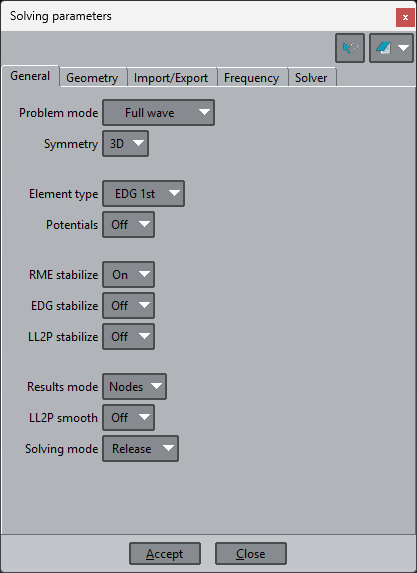
\includegraphics[width=0.41\textwidth]{Contents/Figures/Win-PSettings-1.png}
		\caption{Solving parameters window - Tab: General.}\label{Win-PSettings-1}
	\end{center}
\end{figure}

\newpage

\begin{figure}[H]
	\begin{center}
		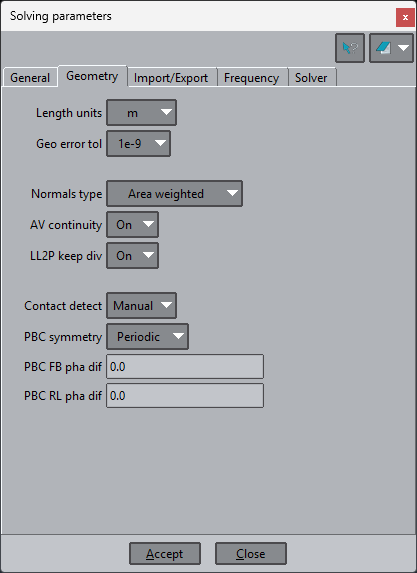
\includegraphics[width=0.41\textwidth]{Contents/Figures/Win-PSettings-2.png}
		\caption{Solving parameters window - Tab: Geometry.}\label{Win-PSettings-2}
	\end{center}
\end{figure}

\begin{figure}[H]
	\begin{center}
		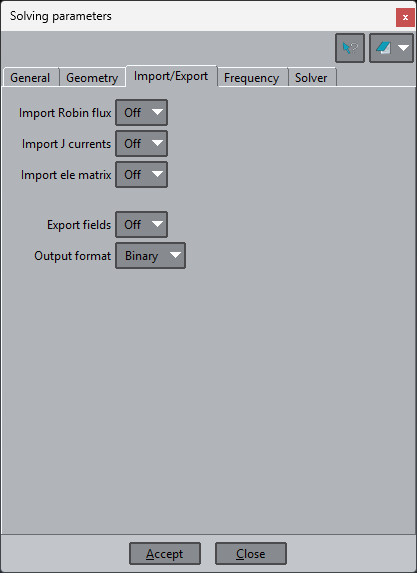
\includegraphics[width=0.41\textwidth]{Contents/Figures/Win-PSettings-3.png}
		\caption{Solving parameters window - Tab: Import/Export.}\label{Win-PSettings-3}
	\end{center}
\end{figure}

\begin{figure}[H]
	\begin{center}
		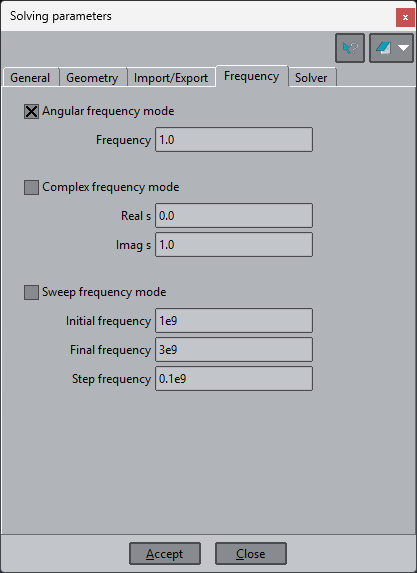
\includegraphics[width=0.41\textwidth]{Contents/Figures/Win-PSettings-4.png}
		\caption{Solving parameters window - Tab: Frequency.}\label{Win-PSettings-4}
	\end{center}
\end{figure}

\begin{figure}[H]
	\begin{center}
		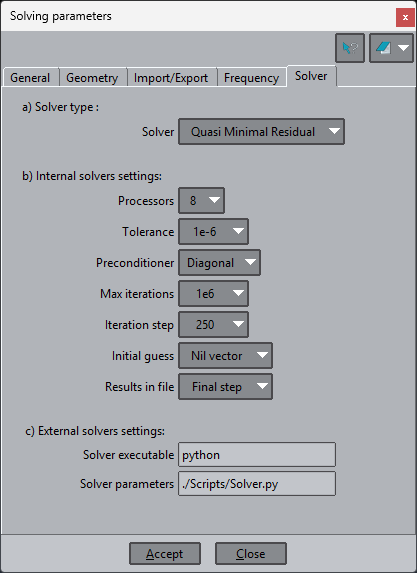
\includegraphics[width=0.41\textwidth]{Contents/Figures/Win-PSettings-5.png}
		\caption{Solving parameters window - Tab: Solver.}\label{Win-PSettings-5}
	\end{center}
\end{figure}

\section{Output results selection}\label{OutputResultsSelection}

The output results of ERMES 20.0 can be presented in three different formats:
\begin{enumerate}\itemsep0em 
	\item Visualization,
	\item Integrals, 
	\item Fields files.
\end{enumerate}
The results for visualization are saved in the problem folder in one binary file \path{.flavia.res}, or in two ASCII files \path{.post.res} and \path{.post.msh}, depending on the output format selected in \ref{ImportExportSettings}-\ref{Win-PSettings-3}. These files can be directly read by the GiD post-processor to display the results, as presented in Chapter \ref{chPostProcess}. The results to be visualized must be specified in the GiD pre-processor windows \ref{Win-Results-1} to \ref{Win-Results-4} before running the simulation. See Section \ref{ssVisualization} for further details.

The results can also be integrated over a surface or volume. This feature is particularly useful for computing parameters such as inductance, capacitance, resistance, total energy dissipation, or scattering parameters \cite{EMF-IJSS, LorentzForceFD, EMPaper-Me}. The surface or volume for field integration must be selected before running the simulation, using windows \ref{Win-Integral-Surfs} and \ref{Win-Integral-Vols}. The values of the integrals will be displayed in the \textit{.info} file and saved in files within the folder \path{\Integrals}, located inside the problem folder. See Sections \ref{ssInfoFile} and \ref{FieldIntegrals} for further details.

Finally, the output results can be saved in ASCII files with a simple format that is easy to read with other applications. These applications can further post-process the results to generate new data tailored for specific purposes. Results from specific regions of the problem domain can be saved in this format by selecting surfaces or volumes using windows \ref{Win-Integral-Surfs} and \ref{Win-Integral-Vols} and enabling the \emph{Export fields} option in \ref{ImportExportSettings}-\ref{Win-PSettings-3}. The files will be saved in a folder named \path{\Fields}, located inside the problem folder, along with information about the nodes and elements in those regions. See Section \ref{ssFieldsOnNodesSel} for further details.

\subsection{Visualization}\label{ssVisualization}

As mentioned above, the results to be visualized in the GiD post-processor must be specified in the GiD pre-processor before running the simulation. This is done from the \textit{Results} window, which can be opened by clicking the corresponding icon on the ERMES menu bar \ref{ERMES-MenuBar}. The \textit{Results} window is divided into four tabs, as shown in Figures \ref{Win-Results-1} to \ref{Win-Results-4}. It is recommended to read Appendix \ref{chEMTheory} in advance to become familiar with the notation.

\subsubsection{Frequency domain results - Figure \ref{Win-Results-1}}

The \textit{Frequency domain} tab is used to select the complex results and their time averages for visualization (see \ref{sEMTH} for further details). These results are stored at the time step t = 0.0 in GiD post-processor. The available options are:

\begin{itemize}\itemsep0.25em 
	\item \textbf{E}: $Real\left[\,\mathbf{E}_{c}(\mathbf{r})\,\,\right]$, $\,Imag\left[\,\mathbf{E}_{c}(\mathbf{r})\,\right]$, $\,\left\|\,\mathbf{E}_{c}(\mathbf{r})\,\right\|$.
	\quad
	\item \textbf{H}: $Real\left[\,\mathbf{H}_{c}(\mathbf{r})\,\right]$, $Imag\left[\,\mathbf{H}_{c}(\mathbf{r})\,\right]$, $\left\|\,\mathbf{H}_{c}(\mathbf{r})\,\right\|$.
	\quad
	\item \textbf{B}: $Real\left[\,\mathbf{B}_{c}(\mathbf{r})\,\right]$, $Imag\left[\,\mathbf{B}_{c}(\mathbf{r})\,\right]$, $\,\left\|\,\mathbf{B}_{c}(\mathbf{r})\,\right\|$.
	\quad
	\item \textbf{J}: $\,Real\left[\,\mathbf{J}_{c}(\mathbf{r})\,\,\right]$, $\,Imag\left[\,\mathbf{J}_{c}(\mathbf{r})\,\,\right]$, $\,\left\|\,\mathbf{J}_{c}(\mathbf{r})\,\,\right\|$, being $\mathbf{J}_{c} = \sigma_{c}\mathbf{E}_{c} + \mathbf{J}_{c}^{imp}$.
	\quad
	\item \textbf{Poynting vector}: $\left\langle\,\mathbf{S}\,\right\rangle = \frac{1}{2}\, Real\left[\,\mathbf{E}_{c}\times\mathbf{\bar{H}}_{c}\,\right]$.
	\quad
	\item \textbf{Joule heating}: $\left\langle\,Q\,\right\rangle =\frac{1}{2}\,\left(\sigma^{'} + \omega\epsilon^{''}\right)\,\left|\,\mathbf{E}_{c}\,\right|^{2}$.
	\quad
	\item \textbf{Lorentz force}: $\left\langle\,\mathbf{f}\,\right\rangle = \frac{1}{2}\, Real\left[\,\mathbf{J}_{c}\times\mathbf{\bar{B}}_{c}\,\right]$.
\end{itemize}

\subsubsection{Time domain results - Figure \ref{Win-Results-2}}

The \textit{Time Domain} tab selects the fields to visualize in time domain. These fields are calculated from the frequency domain results, as in \ref{sEMTH}. These results are stored at the GiD post-processor time steps ranging from t = T/32 to t = T, where $\text{T} = 2\pi/\omega$ is the period of the harmonic oscillation and T/32 is the time step. The textbox showing the time interval in \ref{Win-Results-2} is purely informative. The interval is fixed and cannot be changed from the interface. However, if desired, it can be modified in the template file \path{18-Solve_and_Print.bas} or its corresponding input file \path{Problem_Name-18.dat} (see Sections \ref{ssTemplateFiles} and \ref{ssProblemFiles} for more details). Time domain results can generate large files on problems with large meshes, so use this options with care. The available options are:

\begin{itemize}\itemsep0em 
	\item \textbf{E(t)}: $\mathbf{E}\,(\mathbf{r},t) = Real\,\left[\mathbf{E}_{c}(\mathbf{r})e^{-i\omega t}\,\right]$.
	\quad
	\item \textbf{H(t)}: $\mathbf{H}\,(\mathbf{r},t) = Real\left[\mathbf{H}_{c}(\mathbf{r})e^{-i\omega t}\right]$.
	\quad
	\item \textbf{B(t)}: \,$\mathbf{B}\,(\mathbf{r},t) = Real\left[\mathbf{B}_{c}(\mathbf{r})e^{-i\omega t}\right]$.
	\quad
	\item \textbf{J (t)}: \,$\mathbf{J}\,\,(\mathbf{r},t) = Real\left[\,\mathbf{J}_{c}(\mathbf{r})e^{-i\omega t}\,\right]$.
\end{itemize}

\subsubsection{Cold plasma results - Figure \ref{Win-Results-3}}

The \textit{Cold Plasma} tab adds magnitudes specific to the \textit{Cold Plasma} mode to the \textit{Frequency Domain} and \textit{Time Domain} results. The cold plasma frequency domain results are stored at the GiD post-processor time step t = 0.0, while the cold plasma time domain results are stored at time steps ranging from t = T/32 to t = T. In this context, parallel ($\parallel$) and perpendicular ($\perp$) components are defined with respect to the direction of the external magnetic flux density $B_{e}$. For further details, it is recommended to consult the references \cite{Swanson, Stix}. The available options when the \textit{Cold plasma} mode is selected in \ref{GeneralSettings} are:

\begin{itemize}\itemsep0em 
	\item \textbf{Electron density}: electron density $n_{e}$, as provided in \ref{PlasmaGeometrySettings}.
	\quad
	\item \textbf{External B field}: applied external magnetic flux density $B_{e}$, as provided in \ref{PlasmaGeometrySettings}.
	\quad
	\item \textbf{Permittivity tensor}: real part of the cold plasma tensor components S, P, D, R, and L.
	\quad
	\item \textbf{E perpendicular}: $Real\left[\,\mathbf{E}_{c\perp}(\mathbf{r})\,\,\right]$, $\,Imag\left[\,\mathbf{E}_{c\perp}(\mathbf{r})\,\right]$, $\,\left\|\,\mathbf{E}_{c\perp}(\mathbf{r})\,\right\|$.
	\quad
	\item \textbf{E parallel}: $Real\left[\,\mathbf{E}_{c\parallel}(\mathbf{r})\,\,\right]$, $\,Imag\left[\,\mathbf{E}_{c\parallel}(\mathbf{r})\,\right]$, $\,\left\|\,\mathbf{E}_{c\parallel}(\mathbf{r})\,\right\|$.
	\quad
	\item \textbf{E perpendicular (t)}: $\mathbf{E}_{\perp}(\mathbf{r},t) = Real\,\left[\mathbf{E}_{c\perp}(\mathbf{r})e^{-i\omega t}\,\right]$.
	\quad
	\item \textbf{E parallel (t)}: $\mathbf{E}_{\parallel}(\mathbf{r},t) = Real\,\left[\mathbf{E}_{c\parallel}(\mathbf{r})e^{-i\omega t}\,\right]$.
\end{itemize}

\subsubsection{Electrostatic results - Figure \ref{Win-Results-4}}\label{ElectrostaticResults}

The \textit{Electrostatic} tab specifies the magnitudes to visualize when the \textit{Electrostatic} mode is selected in \ref{GeneralSettings}. It also exports the calculated static current density to a file. This file can later be imported using the \emph{Import currents} option in \ref{ImportExportSettings} to impose the same volumetric current density distribution in \textit{Full Wave} or \textit{Cold Plasma} mode calculations. This feature is particularly useful, for example, when computing quasi-static fields generated by coils with complex geometries. The available options when the \textit{Electrostatic} mode is selected in \ref{GeneralSettings} are:

\begin{itemize}\itemsep0em 
	\item \textbf{Electrostatic potential}: $\phi$.
	\quad
	\item \textbf{Electrostatic E field}: $\mathbf{E} = -\nabla\phi$.
	\quad
	\item \textbf{Electrostatic current density}: $\mathbf{J} = \sigma^{'}\mathbf{E}$.
	\quad
	\item \textbf{Electrostatic Joule heating}: $Q = \sigma^{'}\left|\,\mathbf{E}\,\right|^{2}$.
	\quad
	\item \textbf{Export electrostatic currents}: it writes the calculated electrostatic current density to the file \path{Jsource-nId.dat}, being \path{nId} the number provided in the textbox \textbf{Export Id}. This file will be stored inside the folder \path{\Export_J_Sources} within the problem folder. The current distribution will be multiplied by the phase $e^{i\varphi}$, being $\varphi$ the phase provided in the textbox \textbf{Export Ph}, when imported into \textit{Full Wave} or \textit{Cold Plasma} mode simulations.
\end{itemize}

\begin{figure}[H]
	\begin{center}
		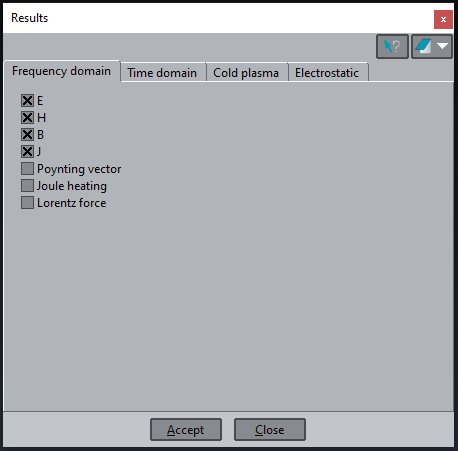
\includegraphics[width=0.57\textwidth]{Contents/Figures/Win-Results-1.png}
		\caption{Results window - Tab: Frequency domain.}\label{Win-Results-1}
	\end{center}
\end{figure}

\begin{figure}[H]
	\begin{center}
		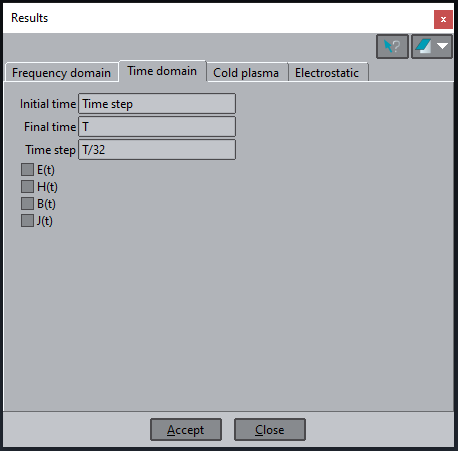
\includegraphics[width=0.57\textwidth]{Contents/Figures/Win-Results-2.png}
		\caption{Results window - Tab: Time domain.}\label{Win-Results-2}
	\end{center}
\end{figure}

\begin{figure}[H]
	\begin{center}
		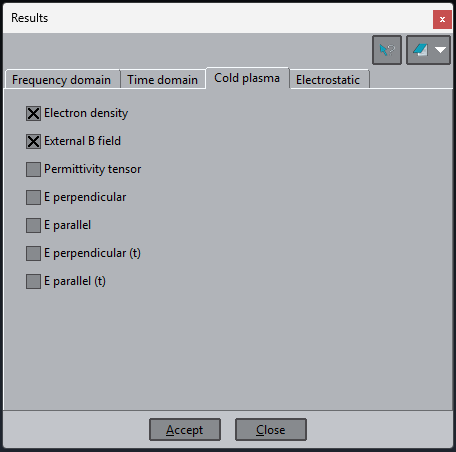
\includegraphics[width=0.57\textwidth]{Contents/Figures/Win-Results-3.png}
		\caption{Results window - Tab: Cold plasma.}\label{Win-Results-3}
	\end{center}
\end{figure}

\begin{figure}[H]
	\begin{center}
		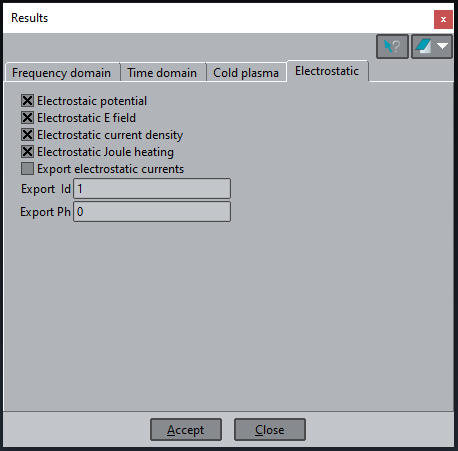
\includegraphics[width=0.57\textwidth]{Contents/Figures/Win-Results-4.png}
		\caption{Results window - Tab: Electrostatic.}\label{Win-Results-4}
	\end{center}
\end{figure}

\subsection{Integrals}\label{FieldIntegrals}

From the \textit{Fields integrals} window of Figures \ref{Win-Integral-Surfs} and \ref{Win-Integral-Vols}, a surface, volume, or waveguide port can be selected over which the fields will be integrated. This window can be opened by clicking on the \textit{Results integrals} icon in the ERMES menu bar \ref{ERMES-MenuBar}. The selection of a surface, volume, or waveguide port follows a procedure similar to that illustrated in Figures \ref{GiD-SelectVolume}, \ref{GiD-CheckMaterials}, \ref{AssignRWPort}, and \ref{CheckRWPort}, but using the \textit{Fields integrals} window \ref{Win-Integral-Surfs}-\ref{Win-Integral-Vols} instead. The results of the calculated integrals will be shown for each frequency in the \path{.info} file and stored in files within the \path{\Integrals} folder, located inside the problem folder. Each surface, volume, or waveguide port will have its own file, named according to its identification number. The type of integrals calculated after selecting a surface, volume, or waveguide port are detailed in the next subsections.

\subsubsection{Surface integrals}\label{ssSurfaceIntSel}

If the option \textit{Field surface integral} in \ref{Win-Integral-Surfs} is assigned to a surface, the following integrals will be automatically calculated:
\begin{itemize}\itemsep0em 
	\item 
	$\,  \iint_{S}\,E_{cx}\,\,dS$, 
	$\,\,\iint_{S}\,E_{cy}\,\,dS$, 
	$\,\,\iint_{S}\,E_{cz}\,\,dS$. 
	
	\item 
	$\,  \iint_{S}\,H_{cx}\,\,dS$, 
	$\,\,\iint_{S}\,H_{cy}\,\,dS$, 
	$\,\,\iint_{S}\,H_{cz}\,\,dS$. 
	
	\item 
	$\,  \iint_{S}\,B_{cx}\,\,dS$, 
	$\,\,\iint_{S}\,B_{cy}\,\,dS$, 
	$\,\,\iint_{S}\,B_{cz}\,\,dS$. 
	
    \item 
    $\,  \iint_{S}\,\,J_{cx}\,\,dS$, 
    $\,\,\iint_{S}\,\,J_{cy}\,\,dS$, 
    $\,\,\iint_{S}\,\,J_{cz}\,\,dS$, 
    $\,\,\iint_{S}\,\,\mathbf{J}_{c}\cdot\,d\mathbf{S}$.
    
    \item 
    $\,  \iint_{S}\,\left|\,\mathbf{E}_{c}\,\right|\,\,dS$, $\,\,\iint_{S}\,\left|\,\mathbf{H}_{c}\,\right|\,\,dS$,
    $\,\,\iint_{S}\,\left|\,\mathbf{B}_{c}\,\right|\,\,dS$,
    $\,\,\iint_{S}\,\left|\,\mathbf{J}_{c}\,\right|\,\,dS$.
    
    \item 
    $\,  \iint_{S}\,\left|\,\mathbf{E}_{c}\,\right|^{2} dS$, $\,\,\iint_{S}\,\left|\,\mathbf{H}_{c}\,\right|^{2} dS$,
    $\,  \iint_{S}\,\left|\,\mathbf{B}_{c}\,\right|^{2} dS$,
    $\,  \iint_{S}\,\left|\,\mathbf{J}_{c}\,\right|^{2} dS$.
    
    \item 
    $\, \iint_{S}\left(\mathbf{E}_{c}\times\mathbf{\bar{H}}_{c}\right)_{x} dS$, 
    $\, \iint_{S}\left(\mathbf{E}_{c}\times\mathbf{\bar{H}}_{c}\right)_{y} dS$,
    $\, \iint_{S}\left(\mathbf{E}_{c}\times\mathbf{\bar{H}}_{c}\right)_{z} dS$,
    $\, \iint_{S}\left(\mathbf{E}_{c}\times\mathbf{\bar{H}}_{c}\right)\cdot\,d\mathbf{S}$.
\end{itemize}
The surface integral results will be available in the \path{Problem_Name.info} file located within the problem folder, where \path{Problem_Name} corresponds to the name of the problem being solved. The results will be also available in files named \path{Surface-sId-Integrals.dat}, where \path{sId} represents the identification number of the surface. These files will be stored in the \path{\Integrals} folder, located within the problem folder. The format of the \path{Surface-sId-Integrals.dat} files will be detailed in Section \ref{ssSurfaceIntFiles}. If the \emph{Sweep frequency mode} is selected, the surface integrals will be calculated for each frequency.

\subsubsection{Scattering parameters}\label{ssScatteringParaSel}

The scattering parameters of a waveguide are automatically calculated if one of the options, \textit{Projection RWTE10} or \textit{Projection CoaxialTEM}, in \ref{Win-Integral-Surfs} is applied to a waveguide port surface. The scattering parameters are obtained using the following equations:
\begin{eqnarray}\label{ProjectionSji}
	S_{ii} &=& \frac{\int_{\Gamma_{i}}\left(\,\mathbf{E}_{c}\,\,\times\mathbf{H}_{m}\,\right)\cdot\mathbf{\hat{n}}\,\,\text{d}\Gamma_{i}}{\int_{\Gamma_{i}}\left(\,\mathbf{E}_{m}\times\mathbf{H}_{m}\,\right)\cdot\mathbf{\hat{n}}\,\,\text{d}\Gamma_{i}} - 1,
	\\\nonumber
	\\
	S_{ji} &=&
	\frac{\int_{\Gamma_{j}}\left(\,\mathbf{E}_{c}\,\,\times\mathbf{H}_{m}\,\right)\cdot\mathbf{\hat{n}}\,\,\text{d}\Gamma_{j}}{\int_{\Gamma_{i}}\left(\,\mathbf{E}_{m}\times\mathbf{H}_{m}\,\right)\cdot\mathbf{\hat{n}}\,\,\text{d}\Gamma_{i}},
\end{eqnarray}
where $i$ and $j$ are the identification number of the ports (see \ref{Win-WG-Rect} and \ref{Win-WG-Coax}), $\Gamma_{i}$ is the surface of the input port, $\Gamma_{j}$ is the surface of the output port, $\mathbf{E}_{c}$ represents the total complex electric field at the port, $\mathbf{E}_{m}$ denotes the electric field of the imposed waveguide mode at the port (see \ref{bsRWPort} and \ref{bsCoaxPort}), and $\mathbf{H}_{m}$ corresponds to the magnetic field of the imposed waveguide mode at the port. The field $\mathbf{H}_{m}$ is obtained from $\mathbf{E}_{m}$ using the time-harmonic Faraday's law (see Appendix \ref{chEMTheory}):
\begin{equation}\label{HmFieldMode}
	\mathbf{H}_{m} = \frac{1}{i\omega\mu}\,\,\nabla\times\mathbf{E}_{m}.
\end{equation}
The scattering parameters results will be available in the \path{Problem_Name.info} file located within the problem folder, where \path{Problem_Name} corresponds to the name of the problem being solved. The results will be also available in files named \path{SParameter-S_j_i.dat}, where \path{j} and \path{i} represent the identification numbers of the ports. These files will be stored in the \path{\Integrals} folder, located within the problem folder. The format of the \path{SParameter-S_j_i.dat} files will be detailed in Section \ref{ssScatteringParaFiles}. If the \emph{Sweep frequency mode} is selected, the scattering parameters will be calculated for each frequency.

\subsubsection{Volume integrals}\label{ssVolIntSel}

If the option \textit{Field volume integral} in \ref{Win-Integral-Vols} is assigned to a volume, the following integrals will be automatically calculated:
\begin{itemize}\itemsep0em 
	\item 
	$\,  \iiint_{V}\,E_{cx}\,\,dV$, 
	$\,\,\iiint_{V}\,E_{cy}\,\,dV$, 
	$\,\,\iiint_{V}\,E_{cz}\,\,dV$. 
	
	\item 
	$\,  \iiint_{V}\,H_{cx}\,\,dV$, 
	$\,\,\iiint_{V}\,H_{cy}\,\,dV$, 
	$\,\,\iiint_{V}\,H_{cz}\,\,dV$. 
	
	\item 
	$\,  \iiint_{V}\,B_{cx}\,\,dV$, 
	$\,\,\iiint_{V}\,B_{cy}\,\,dV$, 
	$\,\,\iiint_{V}\,B_{cz}\,\,dV$. 
	
	\item 
	$\,  \iiint_{V}\,\,J_{cx}\,\,dV$, 
	$\,\,\iiint_{V}\,\,J_{cy}\,\,dV$, 
	$\,\,\iiint_{V}\,\,J_{cz}\,\,dV$.

	\item 
	$\,  \iiint_{V}\,\left|\,\mathbf{E}_{c}\,\right|\,\,dV$, $\,\,\iiint_{V}\,\left|\,\mathbf{H}_{c}\,\right|\,\,dV$,
	$\,\,\iiint_{V}\,\left|\,\mathbf{B}_{c}\,\right|\,\,dV$,
	$\,\,\iiint_{V}\,\left|\,\mathbf{J}_{c}\,\right|\,\,dV$.
	
	\item 
	$\,  \iiint_{V}\,\left|\,\mathbf{E}_{c}\,\right|^{2} dV$, $\,\,\iiint_{V}\,\left|\,\mathbf{H}_{c}\,\right|^{2} dV$,
	$\,  \iiint_{V}\,\left|\,\mathbf{B}_{c}\,\right|^{2} dV$,
	$\,  \iiint_{V}\,\left|\,\mathbf{J}_{c}\,\right|^{2} dV$.

	\item 
	$\, \iiint_{V}\left(\mathbf{J}_{c}\times\mathbf{B}_{c}\right)_{x} dV$, 
	$\, \iiint_{V}\left(\mathbf{J}_{c}\times\mathbf{B}_{c}\right)_{y} dV$,
	$\, \iiint_{V}\left(\mathbf{J}_{c}\times\mathbf{B}_{c}\right)_{z} dV$,
	$\, \iiint_{V}\left|\mathbf{J}_{c}\times\mathbf{B}_{c}\right|     dV$.
	
	\item 
	$\, \iiint_{V}\left(\mathbf{E}_{c}\cdot\mathbf{\bar{J}}_{c}\right) dV$.
\end{itemize}
The scattering parameters results will be available in the \path{Problem_Name.info} file located within the problem folder, where \path{Problem_Name} corresponds to the name of the problem being solved. The results will be also available in files named \path{Volume-vId-Integrals.dat}, where \path{vId} represents the identification number of the volume. These files will be stored in the \path{\Integrals} folder, located within the problem folder. The format of this file will be detailed in Section \ref{ssVolumeIntFiles}. If the \emph{Sweep frequency mode} is selected, the volume integrals will be calculated for each frequency.
\quad\\
\begin{figure}[H]
	\begin{center}
		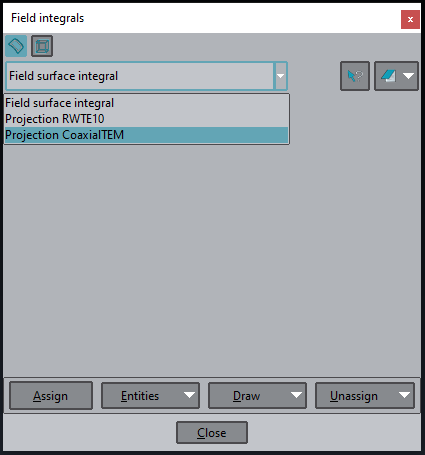
\includegraphics[width=0.57\textwidth]{Contents/Figures/Win-Integral-Surfs.png}
		\caption{Field integrals window - Surfaces.}\label{Win-Integral-Surfs}
	\end{center}
\end{figure}

\begin{figure}[H]
	\begin{center}
		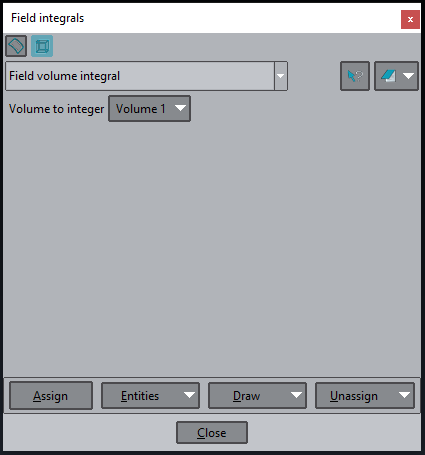
\includegraphics[width=0.57\textwidth]{Contents/Figures/Win-Integral-Vols.png}
		\caption{Field integrals window - Volumes.}\label{Win-Integral-Vols}
	\end{center}
\end{figure}

\subsection{Fields files}\label{ssFieldsOnNodesSel}

If the \emph{Export Fields} option in \ref{ImportExportSettings}-\ref{Win-PSettings-3} is set to \textit{On}, and there are surfaces or volumes with the \textit{Field Surface Integral} or \textit{Field Volume Integral} options assigned to them, the fields $\mathbf{E}{c}$, $\mathbf{B}{c}$, $\mathbf{H}{c}$, and $\mathbf{J}{c}$ for those surfaces or volumes will be saved for each node on those surfaces or volumes in files within the \path{\Fields} folder, located in the problem folder. 

If surfaces are assigned, the fields will be saved to a set of files named \path{Surface_sId_E.dat}, \path{Surface_sId_B.dat}, \path{Surface_sId_H.dat}, and \path{Surface_sId_J.dat}, where \path{sId} represents the surface's identification number. Similarly, if volumes are assigned, the fields will be saved to files named \path{Volume_vId_E.dat}, \path{Volume_vId_B.dat}, \path{Volume_vId_H.dat}, and \path{Volume_vId_J.dat}, where \path{vId} represents the volume's identification number.

Additionally, the following files will be stored in the same folder, providing information about the nodes and elements of the mesh for the selected surfaces and volumes: \path{Surface_sId_Nodes.dat}, \path{Surface_sId_Elements.dat}, \path{Volume_vId_Nodes.dat}, and \path{Volume_vId_Elements.dat}. The format of all these files will be detailed in Section \ref{ssFieldsOnNodesFiles}.

\section{Meshing}

The last step before clicking the \textit{Calculate} button is to mesh the geometry. This must be done after assigning sources, boundary conditions, and materials. Any reassignment of sources, boundary conditions, or materials will require re-meshing of the geometry. This does not include changes in its values; re-meshing is only required if they are reassigned to a different geometric entity. The meshing process can be started by clicking on the \textit{Generate mesh} icon in the ERMES menu bar \ref{ERMES-MenuBar} or from the upper menu of GiD: \textbf{\underline{M}esh} $\rightarrow$ \textbf{Generate mesh...}. The size of the mesh elements must take into account that almost ten elements per wavelength may be necessary to obtain a well defined solution, and that the wavelength changes depending on the medium under consideration according to the following formula for IHL materials:
\begin{equation}\label{WavelenghtIHL}
	\lambda = \frac{c}{f\sqrt{\varepsilon_{r}\mu_{r}}}
\end{equation}
where $f$ is the problem frequency, $c$ is the speed of light in vacuum ($\sim 3x10^{8} \text{m/s}$), $\varepsilon_{r}$ is the relative electric permittivity of the IHL material, and $\mu_{r}$ is the relative magnetic permeability of the IHL material. For cold plasmas, the wavelength depends on the location, plasma conditions and the wave modes that propagate in each region (see references \cite{Swanson, Stix} for further details). 

Different mesh sizes can be assigned to points, lines, surfaces, or volumes from the GiD upper menu: \textbf{\underline{M}esh} $\rightarrow$ \textbf{Unstructured} $\rightarrow$ \textbf{Assign sizes on} [ \textbf{points $\mid$ lines $\mid$ surfaces $\mid$ volumes} ]. The transition speed from one size to another can be modified in the \textit{Preferences Window} \ref{Meshing-Settings-1}, which can be opened from the GiD upper menu: \textbf{\underline{U}tilities} $\rightarrow$ \textbf{Preferences...}. Then, in the left menu of the \textit{Preferences Window}, click on: \textbf{Meshing} $\rightarrow$ \textbf{General}. Additional mesh parameters can be modified from the \textit{Meshing} menu of the \textit{Preferences Window}, as shown in Figure \ref{Meshing-Settings-2}. For further details on meshing with GiD, refer to the tutorials in \textbf{\underline{H}elp} $\rightarrow$ \textbf{Tutorials...} or online \cite{GiDWeb}.

\begin{figure}[H]
	\begin{center}
		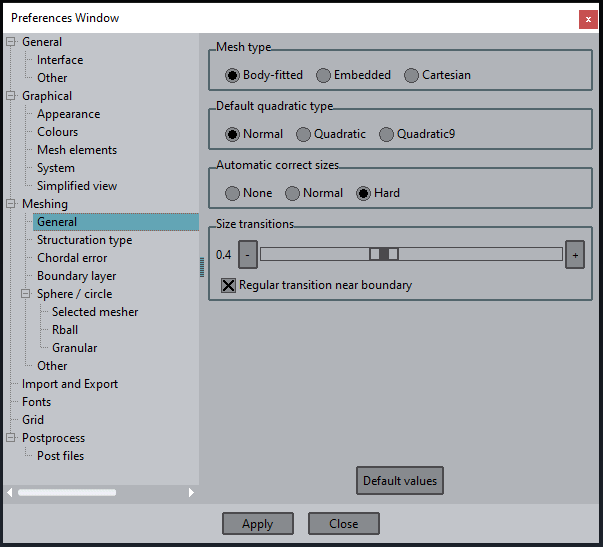
\includegraphics[width=0.52\textwidth]{Contents/Figures/Meshing-Settings-1.png}
		\caption{Preferences window - Meshing - General.}\label{Meshing-Settings-1}
	\end{center}
\end{figure}

\begin{figure}[H]
	\begin{center}
		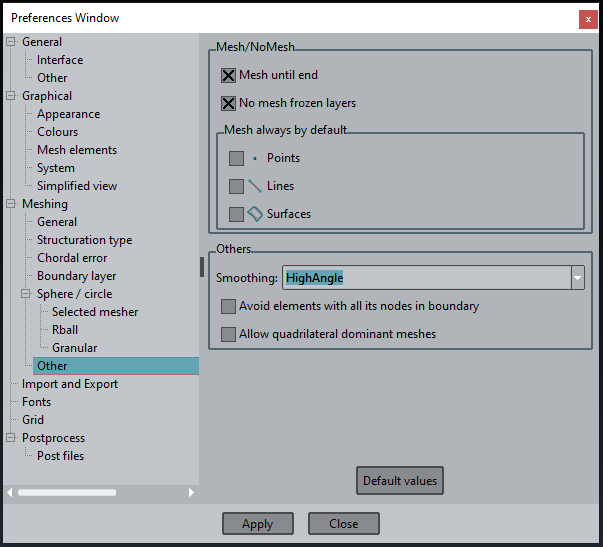
\includegraphics[width=0.52\textwidth]{Contents/Figures/Meshing-Settings-2.png}
		\caption{Preferences window - Meshing - Other.}\label{Meshing-Settings-2}
	\end{center}
\end{figure}

\section{ERMES input files}\label{sERMESInputFiles}

ERMES 20.0 input files are automatically generated when you click the \textit{Calculate} icon in the ERMES menu bar \ref{ERMES-MenuBar}. These files are saved in the problem folder and are re-generated each time you click on the \textit{Calculate} icon. ERMES 20.0 is launched immediately after creating the input files. Alternatively, you can generate the input files without launching ERMES 20.0, via the GiD upper menu: \textbf{\underline{F}iles} $\rightarrow$ \textbf{Export} $\rightarrow$ \textbf{Calculation file...}. This option is especially useful for batch calculations, enabling the user to modify directly input files and run parametrized ERMES simulations without the need of re-opening GiD each time a parameter is changed.

ERMES 20.0 input files are created from a set of templates located in the problem type folder \path{\ERMES.gid}. This set of templates extract data from the GiD pre-processor and generate input files in the problem folder according to the format defined by the templates. The process of creating input files is completely automatic and transparent for a general user. However, advanced users can benefit from a detailed description of this process to further customize ERMES 20.0. This section will describe the templates and input files, as well as additional files required by ERMES 20.0, such as those containing cold plasma electron density and magnetic field distributions, and pre-calculated electric current densities.

\subsection{Template files}\label{ssTemplateFiles}

The problem type folder \path{\ERMES.gid} contains all the essential files required to create the GiD-ERMES 20.0 interface. These files can be edited, allowing for the addition of new windows, data fields, or custom actions to be executed before or after invoking ERMES 20.0. Below is a list of the files that define and control the functionality of the GiD-ERMES 20.0 interface:
\begin{itemize}\itemsep0em 
	\item \path{ERMES.cnd}: defines boundary conditions windows,
	\item \path{ERMES.mat}: defines materials windows,
	\item \path{ERMES.prb}: defines parameters windows,
	\item \path{ERMES.tcl}: defines ERMES menu bar,
	\item \path{ERMES.uni}: defines units,
	\item \path{ERMES.win.bat}: calls ERMES on Windows,
	\item \path{ERMES.unix.bat}: calls ERMES on Linux systems.
\end{itemize}
The directory \path{\ERMES.gid} also contains a set of \path{.bas} template files that process the data provided by the GiD-ERMES interface to create \path{.dat} input files in the specific format required by ERMES 20.0. Below is a list of these template files, along with a brief description of the input data file they generate:
\begin{itemize}\itemsep0em 
	\item \path{ERMES.bas}: problem definition and global settings.
	\item \path{01-Nodes_IdCoords.bas}: list of all mesh nodes.
	\item \path{02-Nodes_Voltages.bas}: list of nodes with a voltage assigned.
	\item \path{03-Nodes_Singular.bas}: list of nodes with a singularity assigned.
	\item \path{04-Volume_Elements.bas}: list of all mesh volumetric tetrahedral elements.
	\item \path{05-SourceJ_Elements.bas}: list of \textbf{J} source volumetric elements.
	\item \path{06-Dirichlet_Elements.bas}: list of PEC, PMC, and TEC surface elements.
	\item \path{07-RobinBC_Elements.bas}: list of Robin condition surface elements.
	\item \path{08-Periodic_Elements.bas}: list of PBC surface elements.
	\item \path{09-Contact_Elements.bas}: list of contact elements.
	\item \path{10-Projector_Elements.bas}: list of projection elements.
	\item \path{11-Materials_Properties.bas}: list of materials and their properties.
	\item \path{12-Cold_Plasma.bas}: cold plasma parameters.
	\item \path{13-Plane_Waves.bas}: plane waves parameters
	\item \path{14-External_Solver.bas}: external solver parameters.
	\item \path{15-Export_Current.bas}: electrostatic export current parameters.
	\item \path{16-Angular_Freq.bas}: angular frequency value.
	\item \path{17-Cmplex_Freq.bas}: complex frequency value.
	\item \path{18-Solve_and_Print.bas}: list of results to visualize.
	\item \path{19-Import_Robin_Elements.bas}: list of imported Robin condition elements.
\end{itemize}
These \path{.bas} template files are thoroughly commented to facilitate easy reading and modification. If an interface other than GiD is preferred, these files serve as the starting point. The \path{.bas} files describe how information is extracted from the GiD interface and how it should be formatted for ERMES 20.0 to read. A new interface would only need to replicate this data acquisition and formatting process.

\subsection{Problem files}\label{ssProblemFiles}

The \path{.bas} template files generate \path{.dat} input files in the problem folder, which are subsequently read by ERMES 20.0 to initiate the calculations. If a problem named \path{Problem_Name} is being solved, the generated input files will be saved in the folder \path{\Problem_Name.gid} and will be named according to the following convention:
\begin{itemize}\itemsep0em 
	\item \path{ERMES.bas} $\rightarrow$ \path{Problem_Name.dat},
    \item \path{01-Nodes_IdCoords.bas} $\rightarrow$ \path{Problem_Name-1.dat},
    \item \path{02-Nodes_Voltages.bas} $\rightarrow$ \path{Problem_Name-2.dat},
    \item \path{03-Nodes_Singular.bas} $\rightarrow$ \path{Problem_Name-3.dat},
    \item \path{04-Volume_Elements.bas} $\rightarrow$ \path{Problem_Name-4.dat},
    \item \path{05-SourceJ_Elements.bas} $\rightarrow$ \path{Problem_Name-5.dat},
    \item \path{06-Dirichlet_Elements.bas} $\rightarrow$ \path{Problem_Name-6.dat},
    \item \path{07-RobinBC_Elements.bas} $\rightarrow$ \path{Problem_Name-7.dat},
    \item \path{08-Periodic_Elements.bas} $\rightarrow$ \path{Problem_Name-8.dat},
    \item \path{09-Contact_Elements.bas} $\rightarrow$ \path{Problem_Name-9.dat},
    \item \path{10-Projector_Elements.bas} $\rightarrow$ \path{Problem_Name-10.dat},
    \item \path{11-Materials_Properties.bas} $\rightarrow$ \path{Problem_Name-11.dat},
    \item \path{12-Cold_Plasma.bas} $\rightarrow$ \path{Problem_Name-12.dat},
    \item \path{13-Plane_Waves.bas} $\rightarrow$ \path{Problem_Name-13.dat},
    \item \path{14-External_Solver.bas} $\rightarrow$ \path{Problem_Name-14.dat},
    \item \path{15-Export_Current.bas} $\rightarrow$ \path{Problem_Name-15.dat},
    \item \path{16-Angular_Freq.bas} $\rightarrow$ \path{Problem_Name-16.dat},
    \item \path{17-Cmplex_Freq.bas} $\rightarrow$ \path{Problem_Name-17.dat},
    \item \path{18-Solve_and_Print.bas} $\rightarrow$ \path{Problem_Name-18.dat}.
    \item \path{19-Import_Robin_Elements.bas} $\rightarrow$ \path{Problem_Name-19.dat}.
\end{itemize}
These files contain all the information required by ERMES 20.0 to perform the simulation. Once created, they can be modified to launch new simulations without the need of further intervention from GiD.

\subsection{Cold plasma files}\label{ColdPlasmaFiles}

The \textit{Cold Plasma} mode requires information about the electron density distribution and the applied static \textbf{B} field. This information is provided through files that must be formatted as described in this section. Examples of the various file formats can also be found in the problem type folder \path{\Documents\Plasma_Files\Plasma_Samples}.

The file format will depend on the \emph{Geometry ext type} selected (see Section \ref{ColdPlasmaMaterial}). As a general rule, lines that start with a number are read and processed by ERMES. Conversely, lines beginning with anything other than a number (e.g., a blank space or the symbol $\#$) are treated as comment lines and ignored by ERMES. Numerical data columns must be separated by one or more blank spaces. When writing these files, it is important to avoid blank spaces at the start of numerical data lines, as a blank space at the beginning of a line will be interpreted as a comment. 

If the \emph{Geometry ext type} option selected is \textit{Flat 1D} or \textit{Curved}, the electron density file must have the following general format:
\begin{small}\begin{lstlisting}
# Comments	 
L(m)   ne(m-3)	
\end{lstlisting}\end{small} 
where \textit{L(m)} represents the column with the distance in meters from the point \textit{L1 00 XYZ} provided in \ref{Win-ColdPlasma-1}, and \textit{ne(m-3)} represents the column with the electron density in $m^{-3}$. For more details on how this file is projected onto the 3D geometry, see Section \ref{ColdPlasmaSettings}. An example of this type of file is provided below:
\begin{small}\begin{lstlisting}
# JPN    95645	 
# Time   48.7	
# L(m)	 ne(m-3)	
0.000   0.00E+00
0.013   0.00E+00
0.027   0.55E+15
0.040   0.96E+16
0.054   1.01E+16
...
\end{lstlisting}\end{small} 
For the applied static \textbf{B} field, if the \emph{Geometry ext type} option selected is \textit{Flat 1D} or \textit{Curved}, the static \textbf{B} field file must have the following general format:
\begin{small}\begin{lstlisting}
# Comments	 
L(m)   B(T)   teta(deg)
\end{lstlisting}\end{small} 
where \textit{L(m)} represents the column with the distance in meters from the point \textit{L1 00 XYZ} using the same distance points as the electron density file above, \textit{B(T)} represents the column with the magnitude of the static \textbf{B} field, and \textit{teta(deg)} represents the column with the angle in degrees formed by the \textbf{B} vector with the plane perpendicular to the tokamak axis \textit{TK axis XYZ}, as viewed from \textit{TK 00 XYZ} towards \textit{L1 00 XYZ}. An example of this type of file is provided below:
\begin{small}\begin{lstlisting}
# JPN    95645	 
# Time   48.7	
# L(m)  B(T)  teta(deg)
0.000   2.55   8.974
0.013   2.56   9.013
0.027   2.57   9.053
0.040   2.58   9.096
0.054   2.59   9.142
...
\end{lstlisting}\end{small} 
If a point falls outside the interval defined by the above files, the last closest values of the electron density distribution and the applied static \textbf{B} field will be assigned to that point. 

If the \emph{Geometry ext type} option is set to \textit{Full 3D}, the electron density and the static \textbf{B} field must be provided at the mesh nodes. The indices and coordinates of these nodes can be found in the problem file \path{Problem_Name-1.dat}. If a node does not have an assigned density or \textbf{B}, it will be assumed to have a zero value. The file for the electron density must have the following general format:
\begin{small}\begin{lstlisting}
# Comments	 
NodeId   ne(m-3) 
\end{lstlisting}\end{small} 
where the column \textit{NodeId} represents the identification number of the mesh nodes, and the column \textit{ne(m-3)} represents the electron density in $m^{-3}$ at the nodes. An example of this type of file is provided below:
\begin{small}\begin{lstlisting}
# Electron density 3D format
# NodeId    ne(m-3)
1    0
2    1.994428193439744e+18
3    6.612102289630953e+18
4    2.230372750985475e+19
5    2.564435389731727e+19
6    2.461668655832341e+19
...
\end{lstlisting}\end{small} 
For the applied static \textbf{B} field, if the \emph{Geometry ext type} option selected is \textit{Full 3D}, the static \textbf{B} field file must have the following general format:
\begin{small}\begin{lstlisting}
# Comments	 
NodeId  Bx(T)  By(T)  Bz(T)
\end{lstlisting}\end{small} 
where \textit{NodeId} represents the column with the identification number of the mesh nodes, and \textit{Bx(T)}, \textit{By(T)}, and \textit{Bz(T)} represents the columns with the Cartesian components of the applied static \textbf{B} field at that node in Tesla. An example of this type of file is provided below:
\begin{small}\begin{lstlisting}
# External B 3D format
# NodeId  Bx(T)  By(T)  Bz(T)
1   -2.097315788269043 -0.8615391254425049  0.32111769914627080
2   -2.060964345932007 -0.9514395594596863  0.32016107439994810
3   -2.141749382019043 -0.8083917498588562  0.33365988731384280
4   -2.279344797134399 -0.6750744581222534  0.36515107750892640
5   -2.329360485076904 -0.8477968573570251  0.37611362338066100
6   -2.203813076019287 -1.0339540243148800  0.38065534830093380
...
\end{lstlisting}\end{small} 
Equilibrium plasma files in \textit{eqdsk} format can be converted into the ERMES 20.0 format using Python scripts. Example scripts for converting \textit{eqdsk} files into the corresponding \textit{Full 3D} format are provided in \path{\Documents\Plasma_Files} along with sample \textit{eqdsk} files.

\subsection{Current density files}

ERMES 20.0 can import an externally computed electric current density distribution, $\mathbf{J}$, and use it as a volumetric source (see Section \ref{ImportExportSettings}). The current density $\mathbf{J}$ must be stored in files located in the problem folder \path{\Export_J_Sources} and saved with the name \path{Jsource-*.dat}, where * is an integer. The mesh used to export $\mathbf{J}$ must match the mesh used in the simulation that imports the current. One option is to export $\mathbf{J}$ directly from the ERMES 20.0 \textit{Electrostatic} mode, as described in Section \ref{ElectrostaticResults}; in this case, the output is automatically formatted to meet the required file specifications. Alternatively, the Python scripts available in the problemtype folder \path{\Documents\Import_Scripts\Current_J_Scripts} can be used to convert current density data from an \textit{eqdsk} plasma equilibrium file into the ERMES 20.0 format. Three different file formats are supported, depending on whether $\mathbf{J}$ is applied element-wise or nodal-wise. The element-wise format supports either a constant or a variable phase for each element. The element-wise constant-phase format is as follows:
\begin{small}\begin{lstlisting}
Phase(rad)
NodeId_1  NodeId_2  NodeId_3  NodeId_4  Jx(A/m2)  Jy(A/m2)  Jz(A/m2)
\end{lstlisting}\end{small} 
where \textit{Phase(rad)} represents the phase $\varphi$ in radians of $\mathbf{J}_{c} = \mathbf{J}e^{i\varphi}$, which is the complex current density imported into ERMES 20.0. \textit{NodeId\_1}, \textit{NodeId\_2}, \textit{NodeId\_3}, and  \textit{NodeId\_4} are the identification numbers of the nodes in a tetrahedral mesh element, and \textit{Jx(A/m2)}, \textit{Jy(A/m2)}, and \textit{Jz(A/m2)} represent the Cartesian components of the \textbf{J} assigned to that element in $A/m^{2}$. An example of this type of file is provided below:
\begin{small}\begin{lstlisting}
0
36  23  32  22  1678.92  1.58440  0.0593253
73  53  54  59  1680.52  10.2272  -0.446468
97  89  92  75  1678.81  11.4579  0.1569060
73  70  77  75  1678.71  9.60589  -0.068501
74  61  59  83  1683.99  12.3864  -0.247362
50  32  34  48  1679.22  5.09186  0.0544152
...
\end{lstlisting}\end{small}
The format above assigns the same phase to all elements in the file. To assign a different phase to each element, the following format must be used:
\begin{small}\begin{lstlisting}
V
NodeId_1 NodeId_2 NodeId_3 NodeId_4  |Jx| Ph_x  |Jy| Ph_y  |Jz| Ph_z
\end{lstlisting}\end{small} 
where the character \textit{V} in the first line indicates the element-wise variable-phase format, $\lvert J_x \rvert$, $\lvert J_y \rvert$, and $\lvert J_z \rvert$ denote the magnitudes of the Cartesian components of $\mathbf{J}$ in $A/m^{2}$, and \textit{Ph\_x}, \textit{Ph\_y}, and \textit{Ph\_z} represent the phases in $rad$ of each Cartesian component. An example of this file format is provided below:
\begin{small}\begin{lstlisting}
V
36  23  32  22  1678.92  0.00  1200.54  3.14  0.1000  1.15
73  53  54  59  1000.00  0.00  1250.26  6.14  0.1500  2.15
97  89  92  75  1500.80  0.00  1330.56  3.16  0.1020  1.30
73  70  77  75  1400.30  0.00  1200.37  2.14  0.1000  1.15
74  61  59  83  1111.32  0.00  1207.26  1.14  0.1300  1.40
50  32  34  48  1600.58  0.00  1102.58  3.10  0.1600  2.15
...
\end{lstlisting}\end{small} 
The third supported format for imported current sources is the nodal-wise format, which is specified as follows: 
\begin{small}\begin{lstlisting}
N
NodeId  |Jx| Ph_x  |Jy| Ph_y  |Jz| Ph_z
\end{lstlisting}\end{small} 
where the symbol \textit{N} in the first line indicates the nodal-wise format; $\lvert J_x \rvert$, $\lvert J_y \rvert$, and $\lvert J_z \rvert$ denote the magnitudes of the Cartesian components of $\mathbf{J}$ in $A/m^{2}$; and \textit{Ph\_x}, \textit{Ph\_y}, and \textit{Ph\_z} represent the phases in $rad$ of each Cartesian component. The indices and coordinates of the mesh nodes can be found in the problem file \path{Problem_Name-1.dat}. If a node does not have an assigned \textbf{J}, it will be assumed to have a zero value. An example of this file format is provided below:
\begin{small}\begin{lstlisting}
N
1  1678.92  0.00  1200.54  3.14  0.1000  1.15
2  1000.00  0.00  1250.26  6.14  0.1500  2.15
3  1500.80  0.00  1330.56  3.16  0.1020  1.30
4  1400.30  0.00  1200.37  2.14  0.1000  1.15
5  1111.32  0.00  1207.26  1.14  0.1300  1.40
6  1600.58  0.00  1102.58  3.10  0.1600  2.15
...
\end{lstlisting}\end{small} 

\section{Batch scripts}

ERMES 20.0 can be called from batch scripts to automate parametrized calculations. Since batch scripts are highly dependent on the operating system, it is recommended to consult the system documentation for proper script syntax, grant executable rights when needed, and address any other configuration requirements before using this option.

Examples of batch scripts used with ERMES 20.0 in High Performance Computer (HPC) clusters can be found in the problemtype folder: \path{\Documents\Batch_Scripts}. These scripts are well-commented, making them easy to understand and adapt for your specific setup. Additionally, there are scripts demonstrating how to use GiD off-screen mode to assign materials, define boundary conditions, and generate the mesh without the GiD graphical interface. 

\section{External solvers}\label{ExternalSolversInfo}

ERMES 20.0 gives the possibility of using external libraries to solve the sparse complex linear system generated by its FEM formulations. The workflow when using external solvers within the GiD user interface is as follows:
\begin{enumerate}\itemsep0em 
	\item User selects \textit{External\_solver} as \textit{Solver\_type} option \ref{SolverSectionTab}.
	\item User sets the rest of problem parameters and clicks on the \textit{Calculate} button.
	\item ERMES 20.0 builds the linear system.
	\item ERMES 20.0 saves the system matrix and vector in the problem folder.
	\item ERMES 20.0 calls the external library.
	\item The external library reads the linear system and solves it.
	\item The external library saves the results vector in the problem folder. 
	\item ERMES 20.0 reads the results vector and generates the results file.
	\item GiD reads the results file for the visualization and analysis of results.
\end{enumerate}
The linear system $A X_{o} = B$ is stored in the problem folder within the following binary files:
\begin{enumerate}\itemsep0em 
	\item \path{Matrix_A_cmplx.bin}: matrix complex coefficients $a_{ij}$,
	\item \path{Matrix_A_int.bin}: matrix indices $ij$,
	\item \path{Matrix_A_aux_cmplx.bin}: auxiliary matrix complex coefficients $c_{mn}$,
    \item \path{Matrix_A_aux_int.bin}: auxiliary matrix indices $mn$,
	\item \path{Vector_B.bin}: linear system vector $B$,
	\item \path{Vector_Xo.bin}: results vector $X_{o}$.
\end{enumerate}
The system matrix is stored in different formats depending on the active problem mode. The available formats are:
\begin{enumerate}\itemsep0.5em 
	\item \textbf{Symmetric}: stores the diagonal and upper diagonal elements of the system matrix in the binary file \path{Matrix_A_cmplx.bin} with the corresponding indices for these elements in the binary file \path{Matrix_A_int.bin}.
	\quad
	\item \textbf{Full-matrix}: stores the entire system matrix in the binary file \path{Matrix_A_cmplx.bin}, along with its corresponding indices in the binary file \path{Matrix_A_int.bin}.
    \quad
	\item \textbf{Hermitic-Symmetric}: stores two separate matrices: the first matrix contains the diagonal and upper-diagonal contributions from the volumetric elements, stored in \path{Matrix_A_cmplx.bin} and \path{Matrix_A_int.bin}. The second matrix contains the diagonal and upper-diagonal contributions from the Robin boundary condition elements, stored in \path{Matrix_A_aux_cmplx.bin} and \path{Matrix_A_aux_int.bin}.	
	\quad
	\item \textbf{Hermitic-Full}: stores two separate matrices: the first matrix contains the diagonal and upper-diagonal contributions from the volumetric elements, saved in \path{Matrix_A_cmplx.bin} and \path{Matrix_A_int.bin}. The second matrix is a complete representation of the contributions from the Robin boundary condition elements, stored in \path{Matrix_A_aux_cmplx.bin} and \path{Matrix_A_aux_int.bin}.
\end{enumerate}
In \textit{Full wave} and \textit{Electrostatic} modes, the stiffness matrix will be always saved in \textit{Symmetric} format. In \textit{Cold plasma} mode, the stiffness matrix can be saved in \textit{Full-matrix}, \textit{Hermitic-Symmetric}, or \textit{Hermitic-Full}, depending on the selection made in \ref{ColdPlasmaSettings}. 

The linear system files described above can be read and transformed to the format required by any external library using the scripts provided in the problemtype folder \path{\External_Solvers}. For instance, in the folder \path{\External_Solvers\Python} there are two examples of Python scripts (\path{SuperLU.py} and \path{BiCG.py}) that use the library Python NumPy \cite{NumPyWeb} to read, transform, and solve the linear system. Further details can be found in the comments written inside those scripts.

The folder \path{\External_Solvers\PETSc} contains all the files required to interface ERMES 20.0 with PETSc \cite{PETScWeb}. It includes the PETSc manual, a \path{README.txt} file with installation instructions, a Bash script for invoking PETSc from the Windows Subsystem for Linux (WSL), and a Python script to read, transform, and solve the linear system generated by ERMES 20.0 using PETSc. In addition, the subfolder \path{\External_Solvers\PETSc\Solver} contains the PETSc executable together with its corresponding C++ source code, \path{PETScSolver.cpp}, which is called by the Python script. Further details are provided in the comments within these files.